%% ================================================================
%%  BSc HONOURS THESIS
%%  Department of Computing and Information Systems
%%  Faculty of Applied Sciences
%%  Sabaragamuwa University of Sri Lanka
%%
%%  Student    : S. Shanthosh   (20APSE4882)
%%  Supervisor : Mrs. W.M.L.S. Abeythunga
%%
%%  Prepared strictly according to:
%%  "Thesis Preparation and Submission Guidelines - Version 1.0"
%%   - Margins  : Left 1.5in, Right/Top/Bottom 1.0in
%%   - Font     : Times New Roman
%%   - Chapter  : ALL CAPS, 14pt, Bold
%%   - Section  : Title Case, 12pt, Bold
%%   - Subsection: Sentence case, 12pt, Bold
%%   - Body     : 12pt, Justified
%%   - Tables/Figures content : 11pt
%%   - Captions : 10pt
%%   - References: IEEE style
%% ================================================================

\documentclass[12pt,a4paper,oneside]{report}

%% ---- Page geometry (Guideline: left 1.5in, others 1.0in) -------
\usepackage[a4paper,left=1.5in,right=1.0in,top=1.0in,bottom=1.0in]{geometry}

%% ---- Times New Roman -------------------------------------------
\usepackage[T1]{fontenc}
\usepackage[utf8]{inputenc}
\usepackage{amsmath}
\usepackage{amssymb}
\usepackage{newtxtext,newtxmath}
%% Latin Modern Mono for \texttt: proper Type1 outlines, avoids
%% the bitmap PK fonts that newtx's txtt falls back to under T1.
\renewcommand{\ttdefault}{lmtt}

%% ---- Core packages ---------------------------------------------
\usepackage{graphicx}
\usepackage{array}
\usepackage{longtable}
\usepackage{multirow}
\usepackage{setspace}
\usepackage{titlesec}
\usepackage{caption}
\usepackage{subcaption}
\usepackage{enumitem}
\usepackage{float}
\usepackage{tabularx}
\usepackage{booktabs}
\usepackage{ragged2e}
\usepackage{tocloft}
\usepackage{fancyhdr}
\usepackage[hidelinks]{hyperref}
\usepackage{listings}
\usepackage{xcolor}

%% ---- Where to look for images ----------------------------------
\graphicspath{{figures/}{../results/}{results/}{./}}

%% ---- Line spacing (1.5) ----------------------------------------
\onehalfspacing

%% ---- Justified body text ---------------------------------------
\justifying
\setlength{\parindent}{0pt}
\setlength{\parskip}{8pt}

%% ---- Page numbering: centred at bottom, no header rule ---------
\pagestyle{plain}
\fancypagestyle{plain}{%
  \fancyhf{}%
  \fancyfoot[C]{\thepage}%
  \renewcommand{\headrulewidth}{0pt}%
  \renewcommand{\footrulewidth}{0pt}%
}

%% ---- Chapter heading: ALL CAPS, 14pt, Bold, centred ------------
\titleformat{\chapter}[display]
  {\centering\normalfont\fontsize{14}{18}\bfseries}
  {CHAPTER \thechapter}
  {10pt}
  {\MakeUppercase}
\titlespacing*{\chapter}{0pt}{-20pt}{28pt}

%% ---- Section heading: Title Case, 12pt, Bold -------------------
\titleformat{\section}
  {\normalfont\fontsize{12}{15}\bfseries}{\thesection}{1em}{}
\titlespacing*{\section}{0pt}{16pt}{8pt}

%% ---- Sub-section heading: Sentence case, 12pt, Bold ------------
\titleformat{\subsection}
  {\normalfont\fontsize{12}{15}\bfseries}{\thesubsection}{1em}{}
\titlespacing*{\subsection}{0pt}{12pt}{6pt}

\titleformat{\subsubsection}
  {\normalfont\fontsize{12}{15}\bfseries\itshape}{\thesubsubsection}{1em}{}

%% ---- Captions: 10pt, sentence case, "Table 3.1: ..." -----------
\captionsetup{
  font={footnotesize},
  labelfont={footnotesize,bf},
  labelsep=colon,
  justification=centering,
  singlelinecheck=true,
  skip=6pt
}
\captionsetup[table]{position=above}
\captionsetup[figure]{position=below}

%% ---- 11pt inside tables ----------------------------------------
%% Tighter inter-column padding keeps the wide results tables
%% inside the 146.5mm text block imposed by the 1.5in left margin.
\newcommand{\tabfont}{\fontsize{11}{13}\selectfont\setlength{\tabcolsep}{4pt}}

%% ---- Column types ----------------------------------------------
\newcolumntype{L}[1]{>{\RaggedRight\arraybackslash}p{#1}}
\newcolumntype{C}[1]{>{\Centering\arraybackslash}p{#1}}
\newcolumntype{R}[1]{>{\RaggedLeft\arraybackslash}p{#1}}

%% ---- Table of contents styling ---------------------------------
\renewcommand{\cftchapfont}{\bfseries}
\renewcommand{\cftchappagefont}{\bfseries}
\renewcommand{\cftchapaftersnum}{.}
\renewcommand{\cftchapdotsep}{\cftdotsep}
\setlength{\cftbeforechapskip}{6pt}

%% ---- ToC / LoT / LoF titles: ALL CAPS, 14pt, bold, centred -----
%%  tocloft supplies its own title typesetting, which bypasses the
%%  titlesec \chapter format, so it is styled explicitly here.
\renewcommand{\cfttoctitlefont}{\hfill\fontsize{14}{18}\bfseries\MakeUppercase}
\renewcommand{\cftlottitlefont}{\hfill\fontsize{14}{18}\bfseries\MakeUppercase}
\renewcommand{\cftloftitlefont}{\hfill\fontsize{14}{18}\bfseries\MakeUppercase}
\renewcommand{\cftaftertoctitle}{\hfill}
\renewcommand{\cftafterlottitle}{\hfill}
\renewcommand{\cftafterloftitle}{\hfill}

%% ---- Front-matter heading helper (unnumbered, ALL CAPS 14pt) ---
%%  Starts a fresh page, records the ToC entry on that page, then
%%  typesets the centred heading.
\newcommand{\frontheading}[1]{%
  \clearpage
  \begin{center}
    {\fontsize{14}{18}\bfseries\MakeUppercase{#1}}
  \end{center}
  \vspace{10pt}
}

%% ---- Code listing style ----------------------------------------
\definecolor{codebg}{RGB}{247,247,247}
\lstset{
  backgroundcolor=\color{codebg},
  basicstyle=\ttfamily\footnotesize,
  breaklines=true,
  frame=single,
  numbers=left,
  numberstyle=\tiny,
  keywordstyle=\bfseries,
  commentstyle=\itshape,
  captionpos=b,
  language=Python,
  showstringspaces=false,
  aboveskip=10pt,
  belowskip=10pt
}

%% ---- Hyperref metadata -----------------------------------------
\hypersetup{
  pdftitle={An Empirical Evaluation of Deep Learning Models for Enhanced and Scalable Bug Detection and Classification in Large-Scale Software Systems},
  pdfauthor={S. Shanthosh}
}

%% ================================================================
\begin{document}

%% ================================================================
%%  COVER PAGE  (Appendix I of the Guidelines)
%% ================================================================
\begin{titlepage}
\thispagestyle{empty}
\centering
\setlength{\parskip}{0pt}
\setstretch{1}

{\fontsize{16}{28.8}\selectfont\bfseries
AN EMPIRICAL EVALUATION OF DEEP LEARNING MODELS FOR ENHANCED AND SCALABLE BUG DETECTION AND CLASSIFICATION IN LARGE-SCALE SOFTWARE SYSTEMS\par}

\vspace{40mm}

{\fontsize{14}{25.2}\selectfont S. Shanthosh\par}

\vspace{10mm}

{\fontsize{14}{25.2}\selectfont 20APSE4882\par}

\vspace{22mm}

{\fontsize{14}{25.2}\selectfont Bachelor of Science Honours Degree in Software Engineering\par}

\vspace{22mm}

{\fontsize{14}{25.2}\selectfont Department of Computing and Information Systems\par}

\vspace{10mm}

{\fontsize{14}{25.2}\selectfont Sabaragamuwa University of Sri Lanka\par}

\vspace{16mm}

{\fontsize{14}{25.2}\selectfont May 2026\par}

\end{titlepage}

%% ================================================================
%%  TITLE PAGE  (Appendix II of the Guidelines)
%% ================================================================
\begin{titlepage}
\thispagestyle{empty}
\centering
\setlength{\parskip}{0pt}
\setstretch{1}

{\fontsize{16}{28.8}\selectfont\bfseries
AN EMPIRICAL EVALUATION OF DEEP LEARNING MODELS FOR ENHANCED AND SCALABLE BUG DETECTION AND CLASSIFICATION IN LARGE-SCALE SOFTWARE SYSTEMS\par}

\vspace{36mm}

{\fontsize{14}{25.2}\selectfont S. Shanthosh\par}

\vspace{10mm}

{\fontsize{14}{25.2}\selectfont 20APSE4882\par}

\vspace{22mm}

{\fontsize{12}{18}\selectfont Thesis submitted in partial fulfillment of the requirements for the degree Bachelor of Science Honours in Software Engineering\par}

\vspace{22mm}

{\fontsize{14}{25.2}\selectfont Department of Computing and Information Systems\par}

\vspace{10mm}

{\fontsize{14}{25.2}\selectfont Sabaragamuwa University of Sri Lanka\par}

\vspace{16mm}

{\fontsize{14}{25.2}\selectfont May 2026\par}

\end{titlepage}

%% ================================================================
%%  Front matter numbering begins at the Declaration (page i),
%%  matching Appendix V of the Guidelines. Cover and title pages
%%  are unnumbered and not counted.
%% ================================================================
\pagenumbering{roman}
\setcounter{page}{1}

%% ================================================================
%%  DECLARATION  (Appendix III of the Guidelines)
%% ================================================================
\frontheading{Declaration}
\addcontentsline{toc}{chapter}{Declaration}

I declare that this thesis does not incorporate, without acknowledgment, any material previously submitted for a Degree or a Diploma in any University and to the best of my knowledge and belief, it does not contain any material previously published or written by another person or myself except where due reference is made in the text.

Also, I hereby grant to Sabaragamuwa University of Sri Lanka the non-exclusive right to reproduce and distribute my thesis, in whole or in part in print, electronic or other medium. I retain the right to use this content in whole or part in future works (such as articles or books).

\vspace{40mm}

\noindent
\begin{tabular}{@{}C{55mm}@{\hspace{20mm}}C{60mm}@{}}
\dotfill & \dotfill \\
Date & Signature \\[4pt]
 & S. Shanthosh (20APSE4882) \\
\end{tabular}

\clearpage

%% ================================================================
%%  CERTIFICATION OF APPROVAL  (Appendix IV of the Guidelines)
%% ================================================================
\frontheading{Certification of Approval}
\addcontentsline{toc}{chapter}{Certification of Approval}

We hereby declare that this thesis is from the student's own work and effort, and all other sources of information used have been acknowledged. This thesis has been submitted with our approval.

\vspace{25mm}

\noindent
\begin{tabular}{@{}L{45mm}@{\hspace{15mm}}L{75mm}@{}}
\dotfill & \dotfill \\
\hfill Date\hfill\mbox{} & Mrs. W.M.L.S. Abeythunga \\
 & Supervisor, \\
 & Department of Computing and Information Systems, \\
 & Faculty of Applied Sciences, \\
 & Sabaragamuwa University of Sri Lanka. \\
\end{tabular}

\vspace{25mm}

\noindent
\begin{tabular}{@{}L{45mm}@{\hspace{15mm}}L{75mm}@{}}
\dotfill & \dotfill \\
\hfill Date\hfill\mbox{} & Head of the Department, \\
 & Department of Computing and Information Systems, \\
 & Faculty of Applied Sciences, \\
 & Sabaragamuwa University of Sri Lanka. \\
\end{tabular}

\clearpage

%% ================================================================
%%  DEDICATION
%% ================================================================
\frontheading{Dedication}
\addcontentsline{toc}{chapter}{Dedication}

\vspace{40mm}
\begin{center}
\textit{To my parents, whose sacrifices made this education possible,}\\[8pt]
\textit{and to my teachers, who taught me to ask better questions.}
\end{center}

\clearpage

%% ================================================================
%%  ACKNOWLEDGEMENTS
%% ================================================================
\frontheading{Acknowledgements}
\addcontentsline{toc}{chapter}{Acknowledgements}

I wish to express my deepest gratitude to my supervisor, Mrs. W.M.L.S. Abeythunga, Department of Computing and Information Systems, Sabaragamuwa University of Sri Lanka, for her invaluable guidance, patience and constructive criticism throughout this research. Her willingness to question my assumptions at every stage improved this work considerably.

I am grateful to the Head and the academic staff of the Department of Computing and Information Systems, Faculty of Applied Sciences, Sabaragamuwa University of Sri Lanka, for providing the academic environment, laboratory facilities and continuous encouragement that made this research possible.

My sincere thanks go to the maintainers of the PROMISE Software Engineering Repository and the OpenML platform for making the JM1 benchmark dataset publicly available for academic research, and to the open-source communities behind PyTorch, scikit-learn, imbalanced-learn and HuggingFace Transformers, whose tools form the technical foundation of every experiment reported in this thesis.

Finally, I thank my family and my friends in the 2020 batch for their support, patience and good humour during the long months of this project.

\vspace{10mm}
\noindent S. Shanthosh\\
May 2026

\clearpage

%% ================================================================
%%  ABSTRACT  (Appendix VIII of the Guidelines, max 300 words)
%% ================================================================
\thispagestyle{plain}
\begin{center}
{\fontsize{12}{18}\selectfont\bfseries Abstract}\\[10pt]
{\fontsize{12}{18}\selectfont\bfseries An Empirical Evaluation of Deep Learning Models for Enhanced and Scalable Bug Detection and Classification in Large-Scale Software Systems}\\[12pt]
{\fontsize{10}{14}\selectfont S. Shanthosh and W.M.L.S. Abeythunga}\\[4pt]
{\fontsize{10}{14}\selectfont\itshape Department of Computing and Information Systems}\\[16pt]
\end{center}
\addcontentsline{toc}{chapter}{Abstract}

{\fontsize{11}{14}\selectfont\setstretch{1.0}
Software defect prediction is constrained by a structural property of defect data that most classifiers are not designed to handle: defective modules are a small minority of any codebase. A model that maximises overall accuracy on such data can appear successful while detecting almost no real defects. This thesis addresses that gap by empirically evaluating traditional machine learning and deep learning models for defect prediction and bug report classification under explicit imbalance correction.

Seven model configurations were trained and evaluated on the JM1 benchmark dataset from the PROMISE repository, comprising 10,885 NASA C-language modules described by 21 Halstead and McCabe complexity metrics with a 4.2:1 class imbalance. Random Forest and Gaussian Naive Bayes served as baselines, each with and without BorderlineSMOTE. A hybrid CNN-LSTM architecture was trained under three loss functions: Binary Cross-Entropy, Focal Loss, and a Class-Weighted Focal Loss proposed in this study, which embeds the observed imbalance ratio directly into the training objective. A DistilBERT transformer was fine-tuned separately for bug report severity classification.

The best traditional baseline, Random Forest with BorderlineSMOTE, achieved a recall of 0.451, detecting 190 of 421 defective modules in the held-out test set. The CNN-LSTM trained with Class-Weighted Focal Loss achieved a recall of 0.834, detecting 351 of 421 defective modules, an improvement of 84.7 percent in detection rate, obtained at a measured cost in precision. Ten-fold stratified cross-validation confirmed the stability of the baseline results. DistilBERT achieved perfect classification on the bug report task.

The findings establish that data-level and algorithm-level imbalance correction are complementary rather than interchangeable, and that combining them substantially outperforms either strategy applied alone.
\par}

\vspace{10pt}
{\fontsize{11}{14}\selectfont\textbf{Keywords:} Software defect prediction, Deep learning, Class imbalance, Focal loss, CNN-LSTM}

\clearpage

%% ================================================================
%%  TABLE OF CONTENTS
%% ================================================================
\renewcommand{\contentsname}{Table of Contents}
\renewcommand{\listtablename}{List of Tables}
\renewcommand{\listfigurename}{List of Figures}

\clearpage
\addcontentsline{toc}{chapter}{Table of Contents}
{\setstretch{1.15}\tableofcontents}
\clearpage

%% ================================================================
%%  LIST OF TABLES
%% ================================================================
\addcontentsline{toc}{chapter}{List of Tables}
{\setstretch{1.15}\listoftables}
\clearpage

%% ================================================================
%%  LIST OF FIGURES
%% ================================================================
\addcontentsline{toc}{chapter}{List of Figures}
{\setstretch{1.15}\listoffigures}
\clearpage

%% ================================================================
%%  LIST OF ABBREVIATIONS  (Appendix IX, alphabetical order)
%% ================================================================
\frontheading{List of Abbreviations}
\addcontentsline{toc}{chapter}{List of Abbreviations}

\begin{center}
\tabfont
\begin{tabular}{L{32mm}L{95mm}}
\toprule
\textbf{Abbreviation} & \textbf{Description} \\
\midrule
AI     & Artificial Intelligence \\
API    & Application Programming Interface \\
AST    & Abstract Syntax Tree \\
AUC    & Area Under the Curve \\
BCE    & Binary Cross-Entropy \\
BERT   & Bidirectional Encoder Representations from Transformers \\
CNN    & Convolutional Neural Network \\
CPU    & Central Processing Unit \\
CV     & Cross-Validation \\
CW-FL  & Class-Weighted Focal Loss \\
DL     & Deep Learning \\
EDA    & Exploratory Data Analysis \\
FL     & Focal Loss \\
FN     & False Negative \\
FP     & False Positive \\
GNN    & Graph Neural Network \\
LIME   & Local Interpretable Model-agnostic Explanations \\
LOC    & Lines of Code \\
LSTM   & Long Short-Term Memory \\
ML     & Machine Learning \\
NB     & Naive Bayes \\
NLP    & Natural Language Processing \\
RF     & Random Forest \\
RNN    & Recurrent Neural Network \\
ROC    & Receiver Operating Characteristic \\
RQ     & Research Question \\
SDLC   & Software Development Life Cycle \\
SDP    & Software Defect Prediction \\
SHAP   & SHapley Additive exPlanations \\
SMOTE  & Synthetic Minority Over-sampling Technique \\
SVM    & Support Vector Machine \\
TN     & True Negative \\
TP     & True Positive \\
XAI    & Explainable Artificial Intelligence \\
\bottomrule
\end{tabular}
\end{center}

\clearpage

%% ================================================================
%%  LIST OF APPENDICES  (Appendix X of the Guidelines)
%% ================================================================
\frontheading{List of Appendices}
\addcontentsline{toc}{chapter}{List of Appendices}

\begin{center}
\tabfont
\begin{tabular}{L{32mm}L{75mm}C{18mm}}
\toprule
\textbf{Appendix} & \textbf{Description} & \textbf{Page} \\
\midrule
Appendix A & Additional experimental results & \pageref{app:a} \\
Appendix B & Source code listings & \pageref{app:b} \\
Appendix C & Software and hardware specifications & \pageref{app:c} \\
Appendix D & Dataset feature dictionary & \pageref{app:d} \\
\bottomrule
\end{tabular}
\end{center}

\clearpage

%% ================================================================
%%  MAIN BODY -- Arabic numerals from page 1
%% ================================================================
\pagenumbering{arabic}
\setcounter{page}{1}

%% ================================================================
%%  CHAPTER 1 -- INTRODUCTION
%% ================================================================
\chapter{Introduction}

\section{Background and Motivation}

The modern software landscape is defined by a scale that was unimaginable when the discipline of software engineering was founded. Contemporary systems routinely comprise millions of lines of code, are developed by geographically distributed teams, and are released under continuous delivery pressures that compress the interval between writing code and running it in production from months to hours. Within this environment, software defects, commonly referred to as bugs, represent both a significant economic cost and a direct threat to system reliability, security and user trust.

The magnitude of this cost is well documented. The Consortium for Information and Software Quality estimates that the annual cost of poor software quality in the United States alone exceeds two trillion dollars, with a substantial proportion attributable to operational failures arising from defects that escaped detection before release \cite{cisq2022}. This figure does not capture the reputational damage and the erosion of user confidence that follow high-profile failures, nor the opportunity cost of engineering effort diverted from feature development into defect remediation.

Critically, the cost of remediating a defect is not constant across the software development life cycle. It escalates sharply with the latency of discovery. Boehm's foundational analysis established that a defect identified during the requirements or design phase costs an order of magnitude less to correct than the same defect discovered after deployment \cite{boehm1981}, a relationship that has been repeatedly confirmed in subsequent empirical work. The practical implication is unambiguous: the earlier a defect is detected, the cheaper it is to fix, and therefore any technique that shifts detection earlier in the life cycle delivers compounding economic returns.

Traditional defect detection methods are increasingly inadequate for systems of the scale described above. Manual code review, although demonstrably effective at identifying subtle logical errors, does not scale to codebases of millions of lines and is constrained by reviewer availability and fatigue. Rule-based static analysis tools scale well computationally but rely on heuristic rule sets that generate high false-positive rates; when developers learn that most warnings are spurious, they begin to ignore all warnings, and the tool's practical value collapses. Dynamic analysis and testing require substantial computational resources and, in principle, cannot guarantee complete coverage of all execution paths in a non-trivial program.

Artificial Intelligence, and specifically the sub-fields of Machine Learning and Deep Learning, has consequently emerged as a promising paradigm for automated defect detection. The underlying premise is that historical software metrics and defect records encode learnable patterns: modules that share measurable structural characteristics with modules known to have been defective are themselves more likely to be defective. A model that learns this relationship can rank modules by predicted fault-proneness, allowing finite testing and review effort to be allocated where it is most likely to be productive.

This premise has been validated repeatedly in the research literature, yet a persistent obstacle limits the practical utility of the resulting models. Defect datasets are, by their nature, severely imbalanced. In a well-engineered system, most modules are not defective. A classifier trained to maximise overall accuracy on such data discovers that the most reliable strategy is to predict the majority class almost always, thereby achieving a high accuracy score while detecting almost none of the defects it was built to find. This thesis is directed at that specific problem.

\section{Purpose of the Study}

\subsection{Aim}

The aim of this study is to empirically evaluate and compare traditional machine learning and deep learning models for software bug detection and classification in large-scale software systems, and to determine the extent to which imbalance-aware training strategies improve the detection of defective modules in severely imbalanced defect datasets.

\subsection{Specific objectives}

The following specific objectives guide this study:

\begin{description}[leftmargin=3em,style=nextline,itemsep=4pt]
  \item[Objective 1:] To implement and evaluate traditional machine learning models, specifically Random Forest and Gaussian Naive Bayes, as baseline software defect predictors on a standard benchmark dataset.
  \item[Objective 2:] To design, implement and evaluate a hybrid Convolutional Neural Network and Long Short-Term Memory (CNN-LSTM) deep learning architecture for software defect prediction from software complexity metrics.
  \item[Objective 3:] To fine-tune and evaluate a DistilBERT transformer model for the automated classification of textual bug reports by severity.
  \item[Objective 4:] To implement and empirically validate imbalance-aware training strategies, specifically Focal Loss and a proposed Class-Weighted Focal Loss, as the primary research contribution of this study.
  \item[Objective 5:] To conduct a rigorous comparative analysis of all model configurations using accuracy, precision, recall, F1-score and ROC-AUC, evaluated on a held-out test set and validated through ten-fold stratified cross-validation.
\end{description}

\section{Statement of the Research Questions}

The study is directed by four research questions. Each is stated below together with the specific measurements that will be conducted to answer it.

\begin{description}[leftmargin=3em,style=nextline,itemsep=6pt]
  \item[RQ1:] \textit{How effectively do traditional machine learning models predict software defects compared to deep learning models in large-scale software systems?}\\
  \textbf{Measurement:} Accuracy, precision, recall, F1-score and ROC-AUC of Random Forest and Gaussian Naive Bayes are compared against the corresponding metrics of the CNN-LSTM architecture, all evaluated on an identical held-out test set of 2,177 modules containing 421 defective instances.

  \item[RQ2:] \textit{How do CNN-LSTM and BERT-based models improve bug detection and classification performance on large, imbalanced software defect datasets?}\\
  \textbf{Measurement:} The recall and F1-score of the CNN-LSTM under three successive loss functions are compared, isolating the marginal contribution of each imbalance-aware component. The DistilBERT model is evaluated separately on the bug report classification task.

  \item[RQ3:] \textit{What is the impact of dataset characteristics and class imbalance on model performance and generalisation?}\\
  \textbf{Measurement:} Recall is measured with and without BorderlineSMOTE for each baseline model, and with and without Focal Loss for the deep learning model, quantifying the isolated and combined effect of data-level and algorithm-level correction. Ten-fold stratified cross-validation quantifies the variance of these estimates.

  \item[RQ4:] \textit{Which model achieves the best balance between accuracy, precision, recall and F1-score for scalable software defect detection and classification?}\\
  \textbf{Measurement:} All seven configurations are ranked on each metric, and the precision-recall trade-off is characterised explicitly in terms of defects detected and false alarms generated per unit of review effort.
\end{description}

\section{Significance of the Study}

The significance of this study rests on four grounds.

First, the class imbalance problem in software defect prediction is widely acknowledged but incompletely addressed. The dominant response in the literature has been data-level correction, principally through variants of the Synthetic Minority Over-sampling Technique. Algorithm-level correction, in which the learning objective itself is modified to weight minority-class errors more heavily, has been extensively studied in computer vision but has received comparatively little systematic attention in the software defect prediction domain. This study supplies that evidence.

Second, existing comparative studies typically evaluate either traditional machine learning against a single deep learning model, or several deep learning architectures against one another. Direct comparison across studies is frustrated by differences in datasets, train-test splits, preprocessing pipelines and evaluation protocols. This study evaluates four model families under strictly identical conditions, with a single fixed random seed, a single preprocessing pipeline and a single held-out test set, so that observed differences are attributable to the models rather than to the experimental setup.

Third, the study addresses both modalities of the software quality assurance problem within a single framework. Defect prediction from code metrics identifies where defects are likely to exist; bug report classification determines how reported defects should be prioritised once discovered. Treating them together permits conclusions about their complementary role that a single-modality study cannot support.

Fourth, and most directly, the study produces actionable guidance for practitioners. The precision-recall trade-off exposed by the results is not an abstract statistical curiosity; it determines how many real defects a team will find and how much wasted review effort it will incur. Quantifying that trade-off allows an engineering organisation to select an operating point deliberately rather than by default.

\section{Definitions}

The following terms are used throughout this thesis with the specific meanings given below.

\begin{description}[leftmargin=0em,style=nextline,itemsep=6pt]
  \item[Software defect (bug):] An error, flaw or fault in a software system that causes it to produce an incorrect or unexpected result, or to behave in an unintended manner. In this study a module is labelled defective if one or more defects were recorded against it in the project's defect tracking record.

  \item[Software defect prediction:] The task of predicting, from measurable properties of a software module, whether that module is likely to contain one or more defects, performed before or independently of executing the module.

  \item[Software metric:] A quantitative measure of a property of software source code. This study uses static complexity metrics, which are computed from the source text without executing it.

  \item[Halstead complexity metrics:] A family of measures derived from counts of distinct and total operators and operands in a program, from which derived quantities including program volume, difficulty, effort and estimated time are computed \cite{halstead1977}.

  \item[Cyclomatic complexity:] A measure of the number of linearly independent paths through a program's control flow graph, introduced by McCabe as an indicator of testing effort and structural complexity \cite{mccabe1976}.

  \item[Class imbalance:] The condition in which the classes of a classification problem are represented in substantially unequal proportions in the training data. The severity of imbalance is expressed here as the ratio of majority-class to minority-class instances.

  \item[Imbalance ratio:] The number of majority-class instances divided by the number of minority-class instances. In the JM1 dataset used in this study the imbalance ratio is 4.2:1.

  \item[Recall (sensitivity):] The proportion of actual defective modules that the model correctly identifies as defective. Recall is the primary evaluation metric in this study because a missed defect is the failure mode of greatest practical consequence.

  \item[Precision:] The proportion of modules predicted defective that are in fact defective. Precision determines the efficiency of the review effort a model's predictions induce.

  \item[Oversampling:] A data-level technique for correcting class imbalance by increasing the number of minority-class instances in the training data, either by duplication or by synthesis.

  \item[SMOTE:] The Synthetic Minority Over-sampling Technique, which generates new minority-class instances by interpolating between existing minority instances and their nearest neighbours in feature space \cite{chawla2002}.

  \item[Focal Loss:] A modification of the standard cross-entropy loss that introduces a modulating factor reducing the loss contribution of examples the model already classifies correctly, thereby concentrating training on difficult examples \cite{lin2017}.

  \item[Transformer:] A neural network architecture based on self-attention mechanisms, which computes representations of each element of a sequence conditioned on all other elements simultaneously rather than sequentially.

  \item[Fine-tuning:] The process of adapting a neural network that has been pre-trained on a large general corpus to a specific downstream task by continuing training on a smaller task-specific dataset.
\end{description}

\section{Delimitations, Limitations, and Assumptions}

\subsection{Delimitations}

Delimitations are the boundaries deliberately imposed on the study by the researcher. This study is delimited as follows.

The primary dataset is restricted to JM1 from the PROMISE repository. This dataset was selected because it is a widely used benchmark that permits comparison with published results, because its size of 10,885 modules is sufficient to train a deep learning model without severe overfitting, and because its 4.2:1 imbalance ratio is representative of the condition the study is designed to investigate. Other PROMISE datasets were not included in the primary evaluation.

The feature representation is restricted to the 21 static complexity metrics supplied with the dataset. Process metrics such as code churn, developer experience and change history were not incorporated, as they are not available in the JM1 distribution.

Only four model families are evaluated: Random Forest, Gaussian Naive Bayes, hybrid CNN-LSTM and DistilBERT. Support vector machines, gradient boosting ensembles and graph neural networks were excluded to keep the comparison tractable and the experimental protocol uniform.

All training and evaluation were performed on a central processing unit. No graphics processing unit was used, which constrains the practical scale of hyperparameter search and the number of training epochs.

\subsection{Limitations}

Limitations are factors outside the researcher's control that constrain the interpretation of the results.

Evaluation on a single dataset means that the generalisability of the findings to other programming languages, application domains and organisational contexts cannot be established from this study alone. Cross-project validation would be required to make such a claim.

The JM1 dataset is derived from NASA software developed under specific engineering standards. Defect labelling practices, module granularity and the definition of a defect may differ in other organisations, and the observed relationships between complexity metrics and defectiveness may not transfer.

The bug report dataset used for the DistilBERT experiment is a structured representative dataset rather than an export from a live defect tracker. Real bug reports contain labelling noise, ambiguous severity assignments and reports whose text does not clearly indicate their severity. Performance on such data would be expected to be lower.

Computational resources restricted the study to CPU-based training, which limited the number of training epochs and the breadth of hyperparameter exploration that could be performed within the project timeframe.

\subsection{Assumptions}

The study proceeds on the following assumptions.

It is assumed that the defect labels supplied with the JM1 dataset are accurate, that is, that modules labelled defective did in fact contain defects and modules labelled clean did not. Label noise in defect datasets is a known concern but cannot be independently verified here.

It is assumed that the 21 static complexity metrics supplied with the dataset are correctly computed and that they carry genuine signal regarding defect-proneness, an assumption supported by the exploratory analysis reported in Chapter 4.

It is assumed that the test set, having been held out before any model fitting and never used for any training or tuning decision, provides an unbiased estimate of generalisation performance on data drawn from the same distribution.

It is assumed that the relationship between complexity metrics and defectiveness is stationary within the dataset, that is, that it does not change systematically across the modules in a way that the random stratified split would fail to represent in both partitions.

\section{Contribution to the Study}

The primary contribution of this thesis is the design and empirical validation of a Class-Weighted Focal Loss for software defect prediction. The proposed loss function extends the standard Focal Loss by introducing a multiplicative class weight equal to the observed imbalance ratio of the training data, thereby correcting for imbalance at two levels simultaneously: at the level of the individual example, through the focusing parameter that down-weights well-classified instances, and at the level of the class, through a weight that encodes the dataset prior directly into the training objective.

Applied to a hybrid CNN-LSTM architecture, this loss function raised recall from 0.451 to 0.834 relative to the strongest traditional machine learning baseline, increasing the number of defective modules detected in the held-out test set from 190 to 351 out of 421. This constitutes an improvement of 84.7 percent in the rate of defect detection.

Beyond this principal result, the study contributes the following to the research field:

\begin{enumerate}[leftmargin=2em,itemsep=4pt]
  \item Quantitative evidence that data-level correction through BorderlineSMOTE and algorithm-level correction through Focal Loss are complementary rather than substitutable, and that their combination outperforms either applied alone.
  \item A controlled comparison of four model families under a single preprocessing pipeline, a single fixed random seed and a single held-out test set, permitting attribution of performance differences to the models themselves.
  \item An explicit characterisation of the precision-recall trade-off induced by increasingly aggressive imbalance correction, expressed in units, defects found and false alarms raised, that are directly interpretable by practitioners.
  \item A fully reproducible experimental framework, comprising six sequential scripts with fixed seeds, which permits independent verification and extension of these results.
\end{enumerate}

\section{Composition of the Thesis}

This thesis is organised into five chapters.

\textbf{Chapter 1} introduces the research problem, states the purpose and specific objectives of the study, formulates the research questions and their associated measurements, establishes the significance of the work, defines the terminology used throughout, and delineates the delimitations, limitations and assumptions under which the study was conducted.

\textbf{Chapter 2} reviews the existing literature. It traces the foundations of software defect prediction from the complexity metrics of Halstead and McCabe through traditional machine learning approaches to contemporary deep learning architectures, surveys the treatment of class imbalance at both the data and algorithm levels, examines the application of transformer models to bug report analysis, and identifies the specific gaps in the literature that this study addresses.

\textbf{Chapter 3} presents the methodology. It describes the research design, the datasets and their collection, the five-stage preprocessing pipeline, the architecture and configuration of every model evaluated, the implementation of the proposed Class-Weighted Focal Loss, and the evaluation framework including the metrics and cross-validation protocol.

\textbf{Chapter 4} reports the results. It presents the exploratory analysis of the dataset, the outcome of preprocessing, the performance of the baseline models both on the held-out test set and under ten-fold cross-validation, the performance of the CNN-LSTM under each of the three loss functions, the performance of DistilBERT on bug report classification, and a comprehensive comparative analysis, concluding with the findings that answer each research question.

\textbf{Chapter 5} discusses the findings and concludes the thesis. It interprets the results in the context of the reviewed literature, draws specific conclusions from the evidence, states the limitations that qualify those conclusions, and recommends directions for further research.

\clearpage

%% ================================================================
%%  CHAPTER 2 -- LITERATURE REVIEW
%% ================================================================
\chapter{Literature Review}

\section{Introduction}

This chapter surveys the body of research on which the present study builds. The review is organised into five substantive sub-topics, each of which contributes a distinct component to the research theme. Section 2.2 examines the foundations of software defect prediction and the traditional machine learning models that constitute the established baseline in this field. Section 2.3 traces the adoption of deep learning architectures for code analysis, from convolutional networks through recurrent networks to hybrid and transformer models. Section 2.4 addresses the class imbalance problem directly, distinguishing data-level from algorithm-level correction strategies. Section 2.5 reviews the separate literature on natural language bug report classification. Section 2.6 sets out the theoretical framework that connects these strands. Section 2.7 identifies the gaps that motivate this study, and Section 2.8 summarises.

\section{Software Defect Prediction}

\subsection{Foundations and early work}

Software defect prediction seeks to identify fault-prone modules before defects manifest in execution, using measurable properties of the code as predictors. The intellectual foundation of the field rests on the proposition, articulated in the 1970s and repeatedly confirmed since, that structural complexity and defect-proneness are systematically related.

Halstead introduced a family of measures derived from counts of operators and operands in a program \cite{halstead1977}. From the four primitive counts, distinct operators, distinct operands, total operators and total operands, Halstead derived program vocabulary, length, volume, difficulty, effort and estimated implementation time. The theoretical claim underlying these measures is that a program's difficulty is a function of the mental effort required to construct and comprehend it, and that this effort correlates with the likelihood of error. Although the psychological theory has been criticised, the metrics themselves have proved to be durable empirical predictors and remain among the most widely used features in defect prediction research.

McCabe proposed cyclomatic complexity as a measure of the number of linearly independent paths through a program's control flow graph \cite{mccabe1976}. For a graph with $E$ edges, $N$ nodes and $P$ connected components, the cyclomatic complexity is $V(G) = E - N + 2P$. McCabe's original motivation was to bound testing effort, since the cyclomatic number gives a lower bound on the number of test cases required for branch coverage. The measure has since been established as a strong univariate predictor of defect density, on the reasoning that modules with many independent paths present more opportunities for a developer to overlook a case.

The consolidation of the field as an empirical discipline owes much to the PROMISE Software Engineering Repository \cite{promise}, which standardised a collection of benchmark defect datasets, including JM1, KC1, PC1 and others derived from NASA software projects. By supplying consistent feature definitions and defect labels in a common format, PROMISE made reproducible comparison across studies possible for the first time and remains the standard evaluation setting for defect prediction research.

\subsection{Traditional machine learning approaches}

Random Forest, introduced by Breiman \cite{breiman2001}, has proved to be among the most consistently effective traditional models for defect prediction. The method constructs an ensemble of decision trees, each fitted to a bootstrap resample of the training data with a random subset of features considered at each split, and aggregates their predictions by majority vote. Two properties make it well suited to software metrics data: the ensemble averaging reduces the variance that individual decision trees exhibit on noisy data, and the random feature subsampling prevents a small number of dominant, mutually correlated metrics from being selected at every split.

Menzies and colleagues conducted a large-scale empirical study of defect prediction from static code features that shaped the subsequent direction of the field \cite{menzies2010}. Their central finding was that the choice of learning algorithm matters less than is commonly supposed, and that simple models applied to appropriately preprocessed features frequently match or exceed the performance of substantially more complex approaches. They further argued that the ceiling on achievable performance is imposed by the information content of the static features themselves rather than by the sophistication of the learner, a claim that motivates the search for richer feature representations.

Gaussian Naive Bayes, despite the evident falsity of its conditional independence assumption when applied to strongly correlated complexity metrics, performs competitively on defect prediction tasks \cite{menzies2010}. Its speed, its lack of hyperparameters and its calibrated probabilistic output make it a valuable baseline, and its comparative robustness on small datasets, where more expressive models overfit, is well documented.

Support vector machines and logistic regression have also been applied to this problem. Both are sensitive to feature scaling and, more importantly for the present study, both optimise objectives that are dominated by the majority class under severe imbalance unless explicitly reweighted.

A consistent finding across this literature is that no single model dominates across all datasets. Performance depends on the dimensionality of the feature space, the size of the dataset and, most decisively, on the degree of class imbalance.

\section{Deep Learning for Code Analysis}

\subsection{Convolutional neural networks}

Convolutional neural networks were developed for image recognition but have been adapted successfully to sequential and structured data. A one-dimensional convolutional layer applies learned filters across a sequence, detecting local patterns irrespective of their position, a property known as translation invariance.

Li applied convolutional networks to defect prediction using both tokenised source code and metric vectors as input, reporting improved F1-scores over traditional machine learning baselines on several PROMISE datasets \cite{li2017}. When applied to a metric vector, the convolutional filters function as detectors of co-occurrence patterns among adjacent metrics, learning, for instance, that a particular combination of elevated volume and elevated branch count is more indicative of defectiveness than either measure considered alone.

The principal limitation of the convolutional approach is that its receptive field is local by construction. Dependencies that span a distance greater than the effective receptive field of the stacked convolutional layers cannot be represented directly. This limitation motivates the incorporation of recurrent components.

\subsection{Recurrent networks and long short-term memory}

Recurrent neural networks process sequences by maintaining a hidden state updated at each step, in principle permitting information to propagate across arbitrary distances. In practice, gradients propagated backwards through many time steps either vanish or explode, which prevents the network from learning long-range dependencies.

Long Short-Term Memory networks, introduced by Hochreiter and Schmidhuber \cite{hochreiter1997}, address this problem through a gated cell state. Three learned gates, forget, input and output, regulate what information is discarded from the cell state, what new information is written to it, and what is exposed to the rest of the network. The additive rather than multiplicative update of the cell state permits gradients to flow across many steps without systematic attenuation.

Thong demonstrated the effectiveness of LSTM networks for bug detection in code snippets, showing that treating code as a sequence and modelling its sequential structure yields improvements over models that treat the same code as an unordered collection of features \cite{thong2018}.

\subsection{Hybrid CNN-LSTM architectures}

The hybrid CNN-LSTM architecture composes the two approaches. Convolutional layers are applied first, extracting local features and producing a sequence of higher-level representations; the LSTM then operates over this derived sequence, modelling dependencies among the extracted features rather than among the raw inputs.

The rationale for this composition is that the two components address complementary limitations. The convolutional layers supply the local pattern detection that the LSTM performs poorly, while the LSTM supplies the long-range dependency modelling that the convolutional layers cannot represent. Empirical results across sequence classification tasks in several domains support the claim that the hybrid outperforms either component in isolation.

In the specific context of defect prediction from metric vectors, the application of a sequential architecture requires interpretation. The 21 metrics of a module do not form a temporal sequence in any physical sense. However, they are ordered consistently across all modules, and the architecture is capable of learning position-specific and position-relative patterns within that fixed ordering. The convolutional layers detect which combinations of nearby metrics are jointly informative, and the LSTM aggregates these detections across the full metric vector.

\subsection{Transformer models}

The introduction of BERT by Devlin and colleagues \cite{devlin2019} substantially altered the landscape of natural language processing tasks in software engineering. BERT dispenses with recurrence entirely, employing a self-attention mechanism in which the representation of each token is computed as a weighted combination of the representations of all tokens in the sequence, with the weights themselves learned and input-dependent. Because attention operates over the whole sequence simultaneously, dependencies of arbitrary length are represented at constant path length, and computation parallelises across the sequence.

BERT is pre-trained on a large unlabelled corpus using masked language modelling and next-sentence prediction objectives, after which it is fine-tuned on a specific downstream task with a comparatively small labelled dataset. This transfer of general linguistic knowledge is the principal source of its effectiveness on tasks with limited labelled data.

Sanh and colleagues introduced DistilBERT, produced by knowledge distillation from BERT \cite{sanh2019}. The distilled model retains approximately 97 percent of BERT's performance on standard benchmarks while reducing parameter count by 40 percent and inference time by 60 percent. For research conducted without dedicated accelerator hardware, this efficiency is decisive.

Subsequent work has applied transformer models to bug report classification \cite{chen2022}, automated program repair and code clone detection, in each case reporting improvements over feature-engineered baselines.

\section{Class Imbalance in Software Defect Data}

Class imbalance is the central obstacle in software defect prediction. Defective modules typically constitute between 5 and 20 percent of a codebase. A classifier trained to minimise overall error on such data finds that predicting the majority class almost always is a highly effective strategy by that criterion, and consequently learns a decision boundary that assigns nearly all modules to the non-defective class.

The consequence is the accuracy paradox: a model reports high accuracy while detecting almost no defects. In the JM1 dataset examined in this study, a classifier that labels every module non-defective achieves 80.7 percent accuracy and detects zero defects. Any evaluation that relies on accuracy as its primary metric is therefore uninformative in this setting, and recall on the minority class must be reported instead.

Two families of correction exist, distinguished by where in the learning pipeline they intervene.

\subsection{Data-level approaches}

Data-level methods modify the training distribution before learning begins. Random undersampling of the majority class balances the classes but discards information, which is costly when the majority class itself exhibits substantial internal variation. Random oversampling of the minority class by duplication preserves all information but provides no new information and tends to induce overfitting to the duplicated instances.

The Synthetic Minority Over-sampling Technique, introduced by Chawla and colleagues \cite{chawla2002}, addresses the limitations of naive duplication by synthesising new minority instances rather than copying existing ones. For each minority instance, SMOTE selects one of its $k$ nearest minority neighbours and generates a new instance at a randomly chosen point on the line segment connecting them in feature space. The synthetic instances are therefore plausible members of the minority class under a local linearity assumption, and the effect is to expand the minority region of the feature space rather than merely to increase its density at existing points.

SMOTE has a well-documented weakness: it treats all minority instances as equally suitable seeds for synthesis. Instances deep within the minority region generate synthetic points that are also deep within that region and therefore contribute little to determining the decision boundary, while noisy minority instances located within the majority region generate synthetic points that actively corrupt the boundary.

BorderlineSMOTE, proposed by Han and colleagues \cite{han2005}, refines the technique by restricting synthesis to minority instances near the class boundary. Each minority instance is classified as safe, in danger or noise according to the proportion of majority instances among its nearest neighbours, and only instances in danger, that is, those on the boundary, are used as seeds. This concentrates the synthetic instances in the region where the decision boundary is actually determined. BorderlineSMOTE is the data-level method adopted in this study.

\subsection{Algorithm-level approaches}

Algorithm-level methods leave the training data unmodified and instead alter the learning objective so that errors on the minority class incur greater cost.

The simplest such method is class weighting, in which the loss contributed by each example is multiplied by a weight inversely proportional to the frequency of its class. This is straightforward to implement and directly counteracts the numerical dominance of the majority class in the aggregate loss.

Focal Loss, introduced by Lin and colleagues \cite{lin2017} for dense object detection, addresses a related but distinct problem. In dense detection, the imbalance between foreground and background candidate regions is extreme, and, critically, the vast majority of background examples are easy: the model classifies them correctly with high confidence early in training. Even though each contributes little individual loss, their sheer number means that in aggregate they dominate the gradient and overwhelm the contribution of the informative hard examples.

Focal Loss introduces a modulating factor that scales the loss down for examples the model already classifies confidently:

\begin{equation}
\mathrm{FL}(p_t) = -\alpha_t \, (1 - p_t)^{\gamma} \, \log(p_t)
\label{eq:focal}
\end{equation}

where $p_t$ denotes the model's estimated probability for the true class, $\alpha_t$ is a class-dependent weighting factor and $\gamma \geq 0$ is the focusing parameter. When $\gamma = 0$ the expression reduces to weighted cross-entropy. As $\gamma$ increases, the factor $(1 - p_t)^{\gamma}$ progressively suppresses the contribution of examples with high $p_t$. At $\gamma = 2$, an example classified with $p_t = 0.9$ contributes one hundredth of the loss it would contribute under standard cross-entropy, whereas an example at $p_t = 0.1$ retains 81 percent of its contribution. The effect is to redirect the gradient signal towards examples the model has not yet learned to classify, which in an imbalanced setting are predominantly minority-class instances.

Focal Loss has been widely adopted in computer vision and, more recently, in natural language processing. Its systematic application to software defect prediction, however, and in particular the combination of its example-level focusing with an explicit class-level weight derived from the observed imbalance ratio, has not been empirically established in this domain. That combination is the contribution of the present study and is formalised in Chapter 3.

\section{Bug Report Classification}

Bug report classification is the task of assigning labels, most commonly severity, priority or defect type, to the natural language text of a defect report. It is a distinct problem from defect prediction: the defect is already known to exist, and the question is how it should be prioritised and routed.

Early approaches represented reports as bag-of-words or TF-IDF vectors and applied support vector machines or logistic regression. These methods are computationally inexpensive and interpretable but discard word order and cannot represent the context-dependence of meaning; the word ``critical'' carries different implications in ``critical security flaw'' and in ``not critical''.

Chen and colleagues demonstrated that fine-tuning BERT on bug report text substantially outperforms TF-IDF approaches \cite{chen2022}. The contextual embeddings capture semantic relationships that static text features cannot, permitting the model to distinguish reports describing severe functional failures from those describing cosmetic issues even when they share surface vocabulary.

Automated bug triage, the assignment of reports to the appropriate developer or team, has been addressed with similar techniques. Recurrent and attention-based models trained on large exports from the Eclipse, Mozilla and JBoss bug trackers consistently outperform keyword-matching heuristics.

A recurring theme in this literature is that reported performance depends heavily on label quality. Severity fields in real trackers are assigned by reporters with varying judgement and are frequently inconsistent, imposing a ceiling on achievable accuracy that is a property of the data rather than of the model.

\section{Theoretical Framework}

The study rests on three connected propositions drawn from the literature reviewed above.

The first is the complexity-defect proposition: measurable structural properties of source code carry information about the likelihood that the code contains defects. This proposition originates with Halstead and McCabe and has been sustained by five decades of empirical work. It licenses the use of static complexity metrics as predictive features and is examined directly in the exploratory analysis of Chapter 4.

The second is the representation proposition: the capacity of a model to exploit the information in those features depends on the class of functions it can represent. Linear and additive models capture the marginal association between individual metrics and defectiveness; models with greater representational capacity, including the hybrid convolutional-recurrent architecture used here, can additionally capture interactions among metrics. This proposition licenses the expectation that deep learning models may extract signal that traditional models cannot.

The third is the objective proposition: what a model learns is determined not only by the data and the architecture but by the objective function it is trained to minimise. Under severe class imbalance, an objective that treats all errors equally will produce a model that neglects the minority class regardless of the data or the architecture. It follows that correcting imbalance requires intervention either in the training distribution or in the objective itself, and that these two interventions are logically independent and may therefore be combined.

The conjunction of these three propositions yields the hypothesis tested in this study: that a high-capacity architecture trained with an objective that corrects for imbalance at both the example level and the class level, on data that has additionally been balanced at the distribution level, will detect substantially more defective modules than a lower-capacity architecture trained with an uncorrected objective on uncorrected data.

\section{Research Gaps}

The review identifies three gaps that this study addresses.

\textbf{Gap 1: Absence of unified comparison under identical conditions.} The literature contains many comparisons of traditional machine learning against deep learning, and many comparisons among deep learning architectures, but few studies that evaluate traditional models, hybrid deep architectures and transformer models on the same data under a single preprocessing pipeline and evaluation protocol. Differences in dataset version, train-test split, feature scaling and metric definition make cross-study comparison unreliable, and the field consequently lacks a controlled account of the relative contribution of model capacity and imbalance correction.

\textbf{Gap 2: Limited application of algorithm-level correction in defect prediction.} Focal Loss is established in computer vision and increasingly in natural language processing, but its application to software defect prediction is sparse. In particular, the variant that combines example-level focusing with a class-level weight set to the observed imbalance ratio, which is the natural extension for a domain where the imbalance ratio is a known and stable property of the data, has not to the author's knowledge been systematically evaluated on standard defect prediction benchmarks.

\textbf{Gap 3: Separation of the code-metric and bug-report modalities.} Defect prediction from code metrics and severity classification of bug reports are treated in largely disjoint literatures, despite addressing consecutive stages of the same quality assurance process. Few studies evaluate both within a single framework, which limits the conclusions that can be drawn about how they might be deployed together.

\section{Summary}

The literature establishes that static complexity metrics carry genuine predictive signal regarding defectiveness; that Random Forest constitutes a strong and difficult-to-beat traditional baseline; that hybrid convolutional-recurrent architectures offer representational advantages over either component alone on sequential feature data; that DistilBERT provides transformer performance at a computational cost compatible with modest hardware; and that class imbalance correction is available at both the data level, principally through BorderlineSMOTE, and the algorithm level, principally through Focal Loss. It further establishes that these two levels of correction have not been systematically combined and evaluated in the defect prediction domain. The methodology described in the following chapter is designed to close that gap.

\clearpage

%% ================================================================
%%  CHAPTER 3 -- METHODOLOGY
%% ================================================================
\chapter{Methodology}

\section{Introduction}

This chapter describes the manner in which the study was conducted. Section 3.2 sets out the research design and the logic by which the experimental configurations were selected. Section 3.3 describes the datasets and their collection. Section 3.4 details the five-stage preprocessing pipeline. Section 3.5 specifies the implementation of every model evaluated, including the proposed Class-Weighted Focal Loss. Section 3.6 defines the evaluation metrics and the data analysis procedures. Section 3.7 summarises the experimental setup.

\section{Research Design}

The study adopts a quantitative, experimental and comparative design. Its logic is that of a controlled experiment: a fixed dataset and a fixed evaluation protocol are held constant while the model architecture and the imbalance correction strategy are varied systematically, so that differences in outcome can be attributed to the manipulated factors.

Seven configurations were evaluated on the code-metric defect prediction task. These are organised as a factorial arrangement over two dimensions. The first dimension is model capacity, comprising Gaussian Naive Bayes, Random Forest and the hybrid CNN-LSTM. The second is imbalance correction, comprising none, data-level correction through BorderlineSMOTE, algorithm-level correction through Focal Loss, and combined data-level and algorithm-level correction through BorderlineSMOTE with Class-Weighted Focal Loss. Not every cell of the full factorial is populated, because Focal Loss is defined only for models trained by gradient descent on a differentiable objective and is therefore inapplicable to Random Forest and Naive Bayes. The populated cells are those that isolate the effect of interest.

The DistilBERT experiment on bug report classification is separate. It uses a different dataset, a different input modality and a different task, and is reported as a parallel investigation addressing the second component of the research question rather than as a competitor in the defect prediction comparison.

Three design decisions govern the validity of the comparison.

First, all models were evaluated on an identical held-out test set, partitioned before any model fitting and never used for training, hyperparameter selection or any other decision. Reported test performance is therefore an unbiased estimate of generalisation.

Second, all preprocessing transformations were fitted exclusively on the training partition and then applied to the test partition. This includes median imputation, winsorisation thresholds and the min-max scaler. No statistic computed from the test set influenced any model.

Third, BorderlineSMOTE was applied exclusively to the training partition. The test set retains its natural 4.2:1 imbalance. Balancing the test set would inflate every reported metric and would misrepresent the condition under which a deployed model would operate.

All random number generators were seeded at 42. The experiment is reproducible.

\section{Data Collection}

\subsection{The JM1 dataset}

The primary dataset is JM1, obtained from the PROMISE Software Engineering Repository \cite{promise} through the OpenML platform \cite{openml}. JM1 comprises static complexity metrics extracted from a NASA real-time predictive ground system implemented in C, together with a binary defect label for each module derived from the project's defect tracking records.

The dataset was retrieved programmatically using the \texttt{fetch\_openml} interface of scikit-learn, ensuring that the exact version used is identifiable and that the retrieval is reproducible. Its properties are summarised in Table \ref{tab:jm1}.

\begin{table}[H]
\centering
\caption{Properties of the JM1 dataset}
\label{tab:jm1}
\tabfont
\begin{tabular}{L{55mm}L{75mm}}
\toprule
\textbf{Property} & \textbf{Value} \\
\midrule
Source                & PROMISE repository (NASA), via OpenML \\
Programming language  & C \\
Total modules         & 10,885 \\
Features              & 21 static complexity metrics \\
Target variable       & \texttt{defects} (binary: 1 = defective, 0 = clean) \\
Defective modules     & 2,106 \quad (19.3\%) \\
Non-defective modules & 8,779 \quad (80.7\%) \\
Imbalance ratio       & 4.2 : 1 \\
Missing values        & 25, across 5 columns \\
\bottomrule
\end{tabular}
\end{table}

The 21 features fall into four groups, listed in Table \ref{tab:features}. A complete data dictionary is provided in Appendix D.

\begin{table}[H]
\centering
\caption{Feature groups in the JM1 dataset}
\label{tab:features}
\tabfont
\begin{tabular}{L{40mm}L{90mm}}
\toprule
\textbf{Group} & \textbf{Features} \\
\midrule
McCabe complexity    & \texttt{v(g)}, \texttt{ev(g)}, \texttt{iv(g)}, \texttt{branchCount} \\
Halstead base        & \texttt{n}, \texttt{v}, \texttt{l}, \texttt{d}, \texttt{i}, \texttt{e}, \texttt{b}, \texttt{t} \\
Code volume          & \texttt{loc}, \texttt{lOCode}, \texttt{lOComment}, \texttt{lOBlank}, \texttt{lOCodeAndComment} \\
Operator and operand & \texttt{uniq\_Op}, \texttt{uniq\_Opnd}, \texttt{total\_Op}, \texttt{total\_Opnd} \\
\bottomrule
\end{tabular}
\end{table}

The dataset was selected for three reasons. It is a widely used benchmark, permitting comparison against published results. Its size is sufficient to train a deep architecture without the severe overfitting that would occur on the smaller PROMISE datasets. And its 4.2:1 imbalance ratio is representative of the condition this study is designed to investigate: severe enough to defeat naive classifiers, but not so extreme as to make the minority class unlearnable.

\subsection{The bug report dataset}

A second dataset of 1,200 bug reports was constructed for the classification task, comprising 600 high-priority and 600 low-priority reports. Each record contains a title field and a description field, concatenated with a separator token for tokenisation. The dataset was generated from twenty distinct structural templates per class, populated with realistic component names, error conditions and reproduction steps, yielding a mean report length of 274 characters.

High-priority reports describe crashes, security vulnerabilities, memory leaks, data corruption and complete loss of function. Low-priority reports describe cosmetic defects, minor inconsistencies in the user interface, documentation errors and non-blocking usability issues.

The use of a constructed rather than a live dataset is a delimitation of the study, stated in Section 1.6, and its implications for the interpretation of the DistilBERT results are addressed in Section 4.7.

\subsection{Sampling method}

No sampling was applied to the JM1 dataset; the complete population of 10,885 modules was used. Partitioning into training and test subsets employed stratified random sampling, which preserves the class proportion of the full dataset within each partition. Stratification is necessary here because simple random sampling of an imbalanced dataset produces partitions whose class ratios vary appreciably by chance, introducing variance into the evaluation that is unrelated to model performance.

\section{Data Preprocessing}

Preprocessing proceeded in five sequential stages. Figure \ref{fig:pipeline_smote} illustrates the effect of the final stage.

\subsection{Stage 1: Missing value imputation}

Twenty-five missing values were present, distributed across five columns: \texttt{uniq\_Op}, \texttt{uniq\_Opnd}, \texttt{total\_Op}, \texttt{total\_Opnd} and \texttt{branchCount}. Each was replaced with the median of its column, computed on the training partition only.

Median imputation was selected over mean imputation because the distributions of software complexity metrics are strongly right-skewed. A small number of very large modules pull the mean substantially above the centre of the distribution, so mean imputation would systematically overstate the complexity of the imputed modules. The median is unaffected by the magnitude of extreme values.

\subsection{Stage 2: Outlier handling by winsorisation}

Complexity metrics contain extreme values corresponding to unusually large or intricate modules. These are genuine observations rather than measurement errors and should not be discarded, but their magnitude distorts the min-max scaling applied subsequently: a single module with a Halstead effort three orders of magnitude above the median would compress every other module into a narrow band near zero.

Winsorisation at the 99th percentile addresses this. For each feature, values exceeding the 99th percentile of the training distribution were replaced by that percentile value. No lower-bound winsorisation was applied, since the metrics are bounded below by zero and exhibit no problematic left tail. All 10,885 modules were retained.

\subsection{Stage 3: Stratified train-test partition}

The dataset was partitioned 80 percent to 20 percent using stratified random sampling with the random seed fixed at 42. The resulting partitions are given in Table \ref{tab:split}.

\begin{table}[H]
\centering
\caption{Training and test partition composition}
\label{tab:split}
\tabfont
\begin{tabular}{L{35mm}C{28mm}C{28mm}C{28mm}}
\toprule
\textbf{Partition} & \textbf{Total} & \textbf{Defective} & \textbf{Non-defective} \\
\midrule
Training & 8,708  & 1,685 & 7,023 \\
Test     & 2,177  & 421   & 1,756 \\
\midrule
Total    & 10,885 & 2,106 & 8,779 \\
\bottomrule
\end{tabular}
\end{table}

\subsection{Stage 4: Min-max normalisation}

All 21 features were rescaled to the interval $[0, 1]$:

\begin{equation}
x' = \frac{x - x_{\min}}{x_{\max} - x_{\min}}
\label{eq:minmax}
\end{equation}

where $x_{\min}$ and $x_{\max}$ are computed from the training partition only. Normalisation is required because the raw features differ in scale by several orders of magnitude, from single-digit cyclomatic complexity values to Halstead effort measures in the hundreds of thousands. Gradient-based optimisation on unnormalised features of such disparate scale converges slowly and unstably, because the loss surface is severely ill-conditioned.

Min-max scaling was chosen over standardisation because, following winsorisation, the features are bounded, and mapping to a fixed interval produces inputs well matched to the activation functions of the network.

\subsection{Stage 5: BorderlineSMOTE}

BorderlineSMOTE \cite{han2005} was applied to the training partition only. The method identified minority instances lying near the class boundary and synthesised 5,338 new defective instances by interpolation, producing a balanced training set of 14,046 instances with 7,023 in each class.

The test partition was not resampled and retains its natural 4.2:1 imbalance, as required for an unbiased estimate of deployed performance.

\begin{figure}[H]
\centering
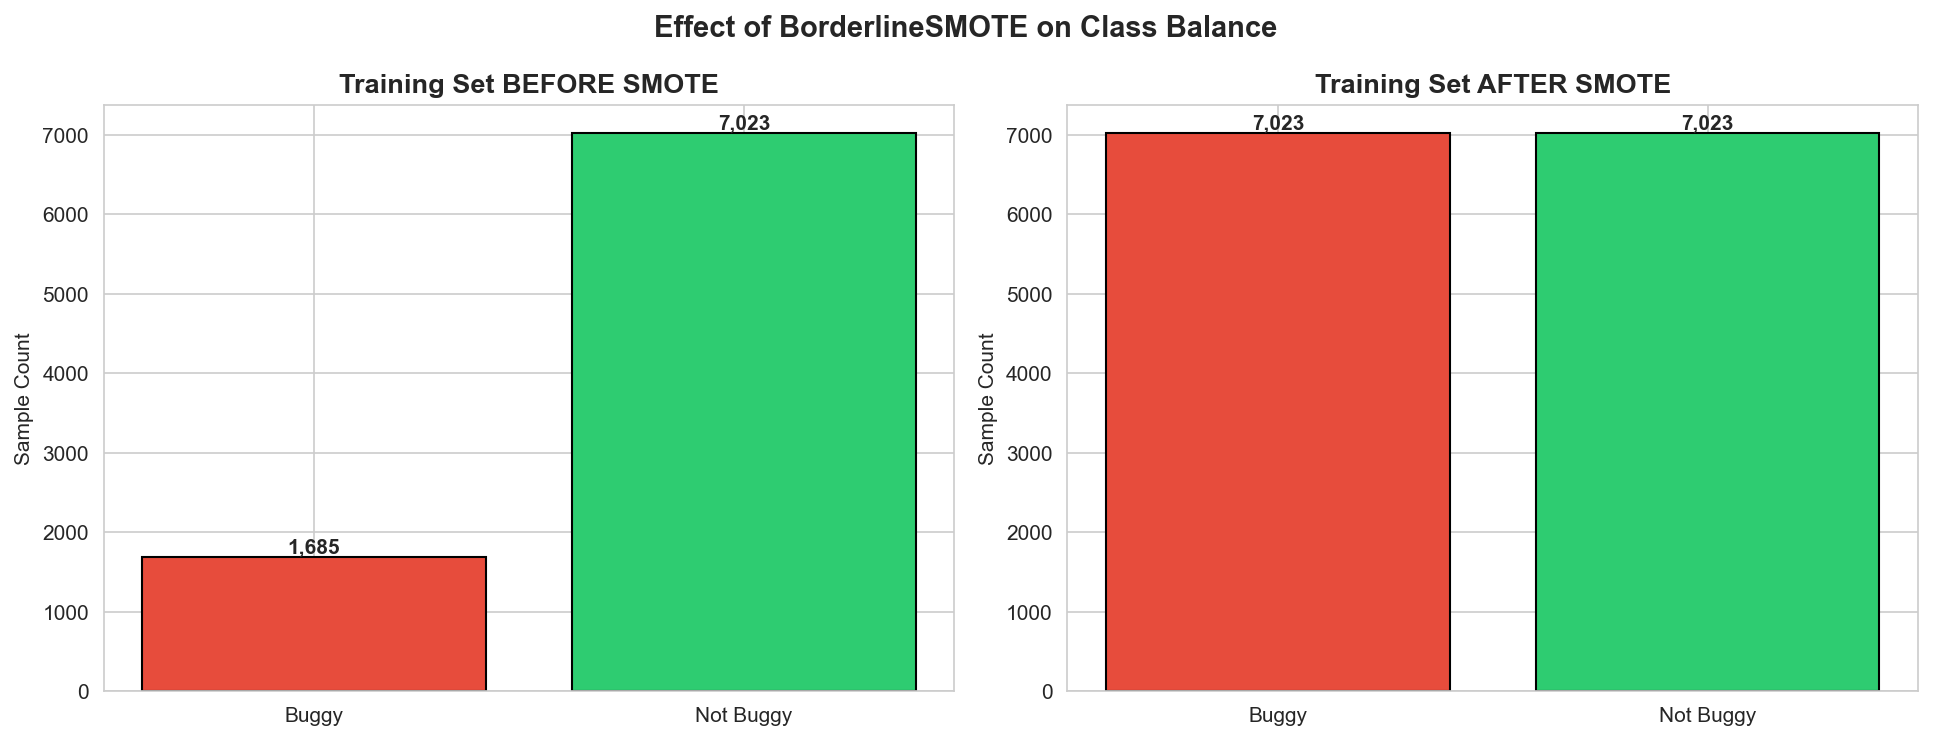
\includegraphics[width=0.8\linewidth]{05_smote_effect.png}
\caption{Effect of BorderlineSMOTE on the training partition. Before resampling the partition contains 8,708 instances of which 1,685 are defective; after resampling it contains 14,046 instances balanced across the two classes}
\label{fig:pipeline_smote}
\end{figure}

\section{Implementation}

\subsection{Development environment}

All experiments were implemented in Python 3.13.2. Table \ref{tab:env} lists the software environment; complete specifications are given in Appendix C.

\begin{table}[H]
\centering
\caption{Software and hardware environment}
\label{tab:env}
\tabfont
\begin{tabular}{L{50mm}L{80mm}}
\toprule
\textbf{Component} & \textbf{Specification} \\
\midrule
Operating system    & Windows 11 Home, build 26200 \\
Python              & 3.13.2 \\
PyTorch             & 2.12.0 (CPU build) \\
scikit-learn        & 1.8.0 \\
imbalanced-learn    & 0.13.0 \\
Transformers        & 5.9.0 (HuggingFace) \\
Hardware            & CPU only, Intel-based workstation \\
Random seed         & 42, all experiments \\
\bottomrule
\end{tabular}
\end{table}

The implementation is organised as six sequential scripts, each corresponding to one phase of the experimental workflow and each writing its outputs to disk so that subsequent phases consume fixed, inspectable intermediate artefacts rather than recomputing them. The scripts are listed in Table \ref{tab:scripts}.

\begin{table}[H]
\centering
\caption{Implementation scripts and their functions}
\label{tab:scripts}
\tabfont
\begin{tabular}{L{48mm}L{82mm}}
\toprule
\textbf{Script} & \textbf{Function} \\
\midrule
\texttt{01\_eda.py}              & Exploratory data analysis and visualisation \\
\texttt{02\_preprocessing.py}    & Five-stage preprocessing pipeline \\
\texttt{03\_baseline\_models.py} & Random Forest and Naive Bayes, four configurations \\
\texttt{04\_cnn\_lstm.py}        & CNN-LSTM under BCE and Focal Loss \\
\texttt{05\_bert.py}             & DistilBERT fine-tuning and evaluation \\
\texttt{06\_final\_enhancement.py} & Class-Weighted Focal Loss and ten-fold cross-validation \\
\bottomrule
\end{tabular}
\end{table}

\subsection{Random Forest}

Random Forest \cite{breiman2001} was implemented using the scikit-learn \texttt{RandomForestClassifier} with 200 estimators, a maximum depth of 15 and the Gini impurity splitting criterion. The depth limit was imposed to constrain the variance of individual trees on this noisy feature space. Two configurations were evaluated, one trained on the unbalanced training partition and one on the BorderlineSMOTE-balanced partition.

\subsection{Gaussian Naive Bayes}

Gaussian Naive Bayes was implemented using the scikit-learn \texttt{GaussianNB} classifier, which models each feature as conditionally Gaussian given the class and applies Bayes' theorem under the conditional independence assumption:

\begin{equation}
P(y \mid x_1, \ldots, x_n) \propto P(y) \prod_{i=1}^{n} P(x_i \mid y)
\label{eq:nb}
\end{equation}

As with Random Forest, two configurations were evaluated, with and without BorderlineSMOTE.

\subsection{Hybrid CNN-LSTM architecture}

The hybrid model was implemented in PyTorch as a subclass of \texttt{nn.Module}. The input feature vector of 21 metrics is reshaped to a sequence of 21 steps with a single channel, permitting the convolutional layers to operate across the metric dimension. The architecture is specified in Table \ref{tab:arch}.

\begin{table}[H]
\centering
\caption{Architecture of the hybrid CNN-LSTM model}
\label{tab:arch}
\tabfont
\begin{tabular}{L{28mm}L{45mm}L{58mm}}
\toprule
\textbf{Layer} & \textbf{Configuration} & \textbf{Function} \\
\midrule
Input       & (batch, 21, 1)        & Normalised complexity metrics \\
Conv1D      & 64 filters, kernel 3  & Local pattern detection \\
BatchNorm   & 64 channels           & Training stabilisation \\
ReLU        & No parameters         & Non-linear activation \\
Conv1D      & 128 filters, kernel 3 & Higher-order feature extraction \\
BatchNorm   & 128 channels          & Training stabilisation \\
ReLU        & No parameters         & Non-linear activation \\
LSTM        & 64 hidden units       & Sequential dependency modelling \\
Dropout     & rate 0.4              & Regularisation \\
Dense       & 32 units, ReLU        & Feature compression \\
Output      & 1 unit, sigmoid       & Defect probability \\
\bottomrule
\end{tabular}
\end{table}

The model contains 77,121 trainable parameters. Batch normalisation follows each convolutional layer to stabilise the distribution of activations during training and permit a higher learning rate. Dropout at rate 0.4 is applied to the LSTM output, a comparatively high rate justified by the small parameter count relative to the training set size and by the risk of overfitting to the synthetic instances introduced by SMOTE.

Training used the Adam optimiser. The learning rate was 0.001 for the BCE and Focal Loss configurations with a \texttt{ReduceLROnPlateau} schedule of patience 3, and 0.0005 for the Class-Weighted Focal Loss configuration with a cosine annealing schedule. Batch size was 256 throughout.

\subsection{Loss functions}

Three loss functions were evaluated, forming a progression in which each adds one component of imbalance correction to the previous.

\textbf{Binary Cross-Entropy} serves as the uncorrected reference:

\begin{equation}
\mathrm{BCE}(p, y) = -\bigl[\, y \log(p) + (1 - y)\log(1 - p) \,\bigr]
\label{eq:bce}
\end{equation}

Every example contributes equally, irrespective of class or difficulty.

\textbf{Focal Loss} \cite{lin2017} introduces example-level correction as given in Equation \ref{eq:focal}, with $\alpha = 0.75$ and $\gamma = 2.0$. The value $\alpha = 0.75$ assigns three times the weight to the minority class; $\gamma = 2.0$ is the value Lin and colleagues found optimal across their experiments and provides substantial but not extreme suppression of easy examples.

\textbf{Class-Weighted Focal Loss}, proposed in this study, adds class-level correction on top of the example-level focusing:

\begin{equation}
\mathrm{CWFL}(p_t, y) = w(y) \cdot \bigl[ -\alpha_t (1 - p_t)^{\gamma} \log(p_t) \bigr]
\label{eq:cwfl}
\end{equation}

where the class weight is

\begin{equation}
w(y) =
\begin{cases}
\rho & \text{if } y = 1 \quad \text{(defective)} \\
1 & \text{if } y = 0 \quad \text{(non-defective)}
\end{cases}
\label{eq:weight}
\end{equation}

and $\rho = 4.2$ is the imbalance ratio observed in the dataset.

The rationale for this construction is that Focal Loss and class weighting correct for different aspects of the same problem. The focusing term $(1 - p_t)^{\gamma}$ acts on individual examples according to how well the model currently classifies them, and is therefore adaptive: its effect changes as training progresses and examples become easier. The class weight $w(y)$ acts on the class as a whole according to a fixed property of the dataset, and is therefore static. An example that is both a minority instance and difficult receives both corrections; an example that is a minority instance but has become easy retains the class-level correction even after the focusing term has suppressed its example-level contribution. Setting $\rho$ to the observed imbalance ratio makes the aggregate loss contribution of the two classes approximately equal before focusing is applied, encoding the dataset prior directly into the objective.

The implementation is given in Listing \ref{lst:cwfl} in Appendix B.

\subsection{DistilBERT fine-tuning}

DistilBERT-base-uncased \cite{sanh2019} was loaded from the HuggingFace model hub and fine-tuned for binary sequence classification with a linear classification head over the pooled representation. Bug reports were tokenised to a maximum length of 128 tokens with padding and truncation. Fine-tuning used the AdamW optimiser with learning rate $2 \times 10^{-5}$, weight decay 0.01 and a linear warmup over the first 10 percent of steps, for 4 epochs at batch size 16, giving 240 total optimisation steps of which 24 were warmup. The model contains 66.9 million parameters.

\section{Data Analysis}

\subsection{Nature of the data}

The data analysed in this study are quantitative and secondary. The JM1 dataset is secondary data, collected by NASA during software development and curated by the PROMISE repository; it was not gathered by the researcher. The features are continuous and discrete numerical measurements, and the target variable is binary and categorical. The bug report dataset is primary in the sense that it was constructed for this study, but its content is synthetic rather than observational.

Because the data are entirely quantitative and the target is categorical, the analysis is a supervised binary classification problem, and the analytical procedures are those of predictive modelling and statistical evaluation rather than of inferential hypothesis testing on population parameters.

\subsection{Evaluation metrics}

All metrics derive from the confusion matrix, whose four cells for this problem are: true positives, defective modules correctly identified; false negatives, defective modules missed; false positives, clean modules incorrectly flagged; and true negatives, clean modules correctly passed. Table \ref{tab:metrics} defines the five metrics reported.

\begin{table}[H]
\centering
\caption{Evaluation metrics and their interpretation}
\label{tab:metrics}
\tabfont
\begin{tabular}{L{25mm}L{38mm}L{68mm}}
\toprule
\textbf{Metric} & \textbf{Definition} & \textbf{Interpretation in this study} \\
\midrule
Accuracy  & $\dfrac{TP+TN}{TP+TN+FP+FN}$ & Overall correctness. Misleading under imbalance and reported only for completeness \\[8pt]
Precision & $\dfrac{TP}{TP+FP}$ & Proportion of flagged modules that are genuinely defective. Determines review efficiency \\[8pt]
Recall    & $\dfrac{TP}{TP+FN}$ & Proportion of defective modules detected. \textbf{Primary metric} \\[8pt]
F1-score  & $\dfrac{2 \cdot P \cdot R}{P+R}$ & Harmonic mean of precision and recall. \textbf{Primary metric} \\[8pt]
ROC-AUC   & Area under the ROC curve & Threshold-independent ranking quality \\
\bottomrule
\end{tabular}
\end{table}

Recall is designated the primary metric on the following reasoning. The two error types have asymmetric costs in this application. A false positive causes a developer to review a module that proves to be clean, costing a bounded amount of time. A false negative causes a defective module to reach production, where its cost is determined by the consequences of the defect and, following Boehm \cite{boehm1981}, is an order of magnitude greater than the cost of detection during development. An evaluation that weights the two errors equally therefore does not reflect the decision problem the model is intended to support.

Accuracy is reported but is not used to rank models. Its inadequacy in this setting is demonstrated directly by the results in Section 4.4.

\subsection{Cross-validation}

Ten-fold stratified cross-validation was applied to the two baseline models to quantify the variance of the performance estimates. The training data are partitioned into ten folds preserving the class ratio; the model is fitted ten times, each time on nine folds and evaluated on the tenth. Results are reported as the mean and standard deviation across folds.

The purpose is to establish whether the single held-out test estimate is representative or an artefact of a fortunate partition. A small standard deviation across folds indicates that performance is stable with respect to the choice of training sample.

Cross-validation was not applied to the deep learning models. Each CNN-LSTM configuration requires substantially longer to train than a Random Forest, and ten-fold cross-validation of all three configurations was not feasible within the computational budget available on CPU-only hardware. This is stated as a limitation in Section 5.5.

\subsection{Analytical procedure}

Analysis proceeded in four steps. First, exploratory analysis characterised the distribution of each feature by class and quantified the imbalance. Second, each model was fitted on the training partition and evaluated on the test partition, producing the five metrics and a confusion matrix. Third, the absolute number of defective modules detected was recorded for each model, providing a directly interpretable measure alongside the ratios. Fourth, models were compared pairwise on recall and F1-score, with differences attributed to the single factor by which the configurations differ.

\section{Summary}

The methodology establishes a controlled comparison across seven configurations spanning three levels of model capacity and four imbalance correction strategies, evaluated on a single held-out test set under a preprocessing pipeline fitted exclusively on training data, with all random seeds fixed. The proposed Class-Weighted Focal Loss combines example-level focusing with a class-level weight equal to the observed imbalance ratio. The following chapter reports the results.

\clearpage

%% ================================================================
%%  CHAPTER 4 -- RESULTS AND FINDINGS
%% ================================================================
\chapter{Results and Findings}

\section{Introduction}

This chapter presents the results of the experiments described in Chapter 3, in the order in which the research questions were stated. Section 4.2 reports the exploratory analysis of the dataset. Section 4.3 reports the outcome of preprocessing. Section 4.4 reports baseline model performance on the held-out test set and Section 4.5 the corresponding cross-validation results. Section 4.6 reports the CNN-LSTM results under each loss function. Section 4.7 reports the DistilBERT results. Section 4.8 presents the comprehensive comparison, and Section 4.9 states the findings that answer each research question.

\section{Exploratory Data Analysis}

\subsection{Class distribution}

The JM1 dataset contains 10,885 modules of which 2,106, or 19.3 percent, are labelled defective. The imbalance ratio is 4.2 majority instances for every minority instance. Figure \ref{fig:classdist} shows the distribution.

\begin{figure}[H]
\centering
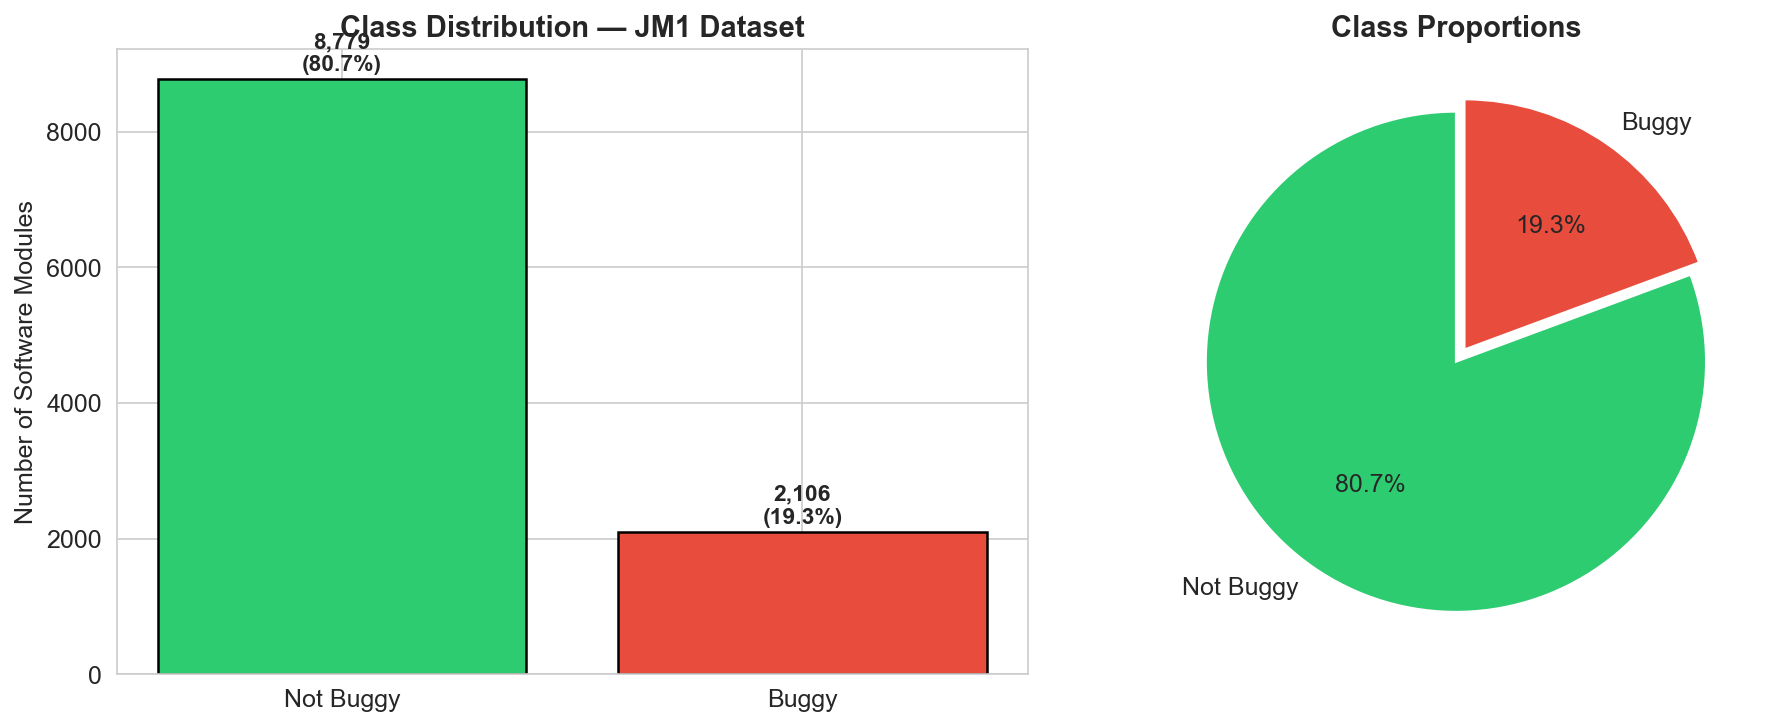
\includegraphics[width=0.72\linewidth]{01_class_distribution.png}
\caption{Class distribution in the JM1 dataset, showing 8,779 non-defective and 2,106 defective modules}
\label{fig:classdist}
\end{figure}

The practical consequence of this distribution is direct and is worth stating numerically. A classifier that labels every module non-defective, without examining any feature, achieves an accuracy of 80.7 percent while detecting none of the 2,106 defective modules. Any model reporting accuracy below this figure is, on that metric alone, worse than a constant prediction, and any model reporting accuracy near it has demonstrated nothing. This observation governs the interpretation of every result reported in this chapter.

\subsection{Feature distributions by class}

Analysis of the feature distributions confirms that the complexity metrics carry genuine signal. Twenty of the 21 features exhibit significantly elevated mean values in defective modules relative to clean modules. Figure \ref{fig:featdist} shows the distributions for the most discriminative features and Figure \ref{fig:featratio} the ratio of class means for all features.

\begin{figure}[H]
\centering
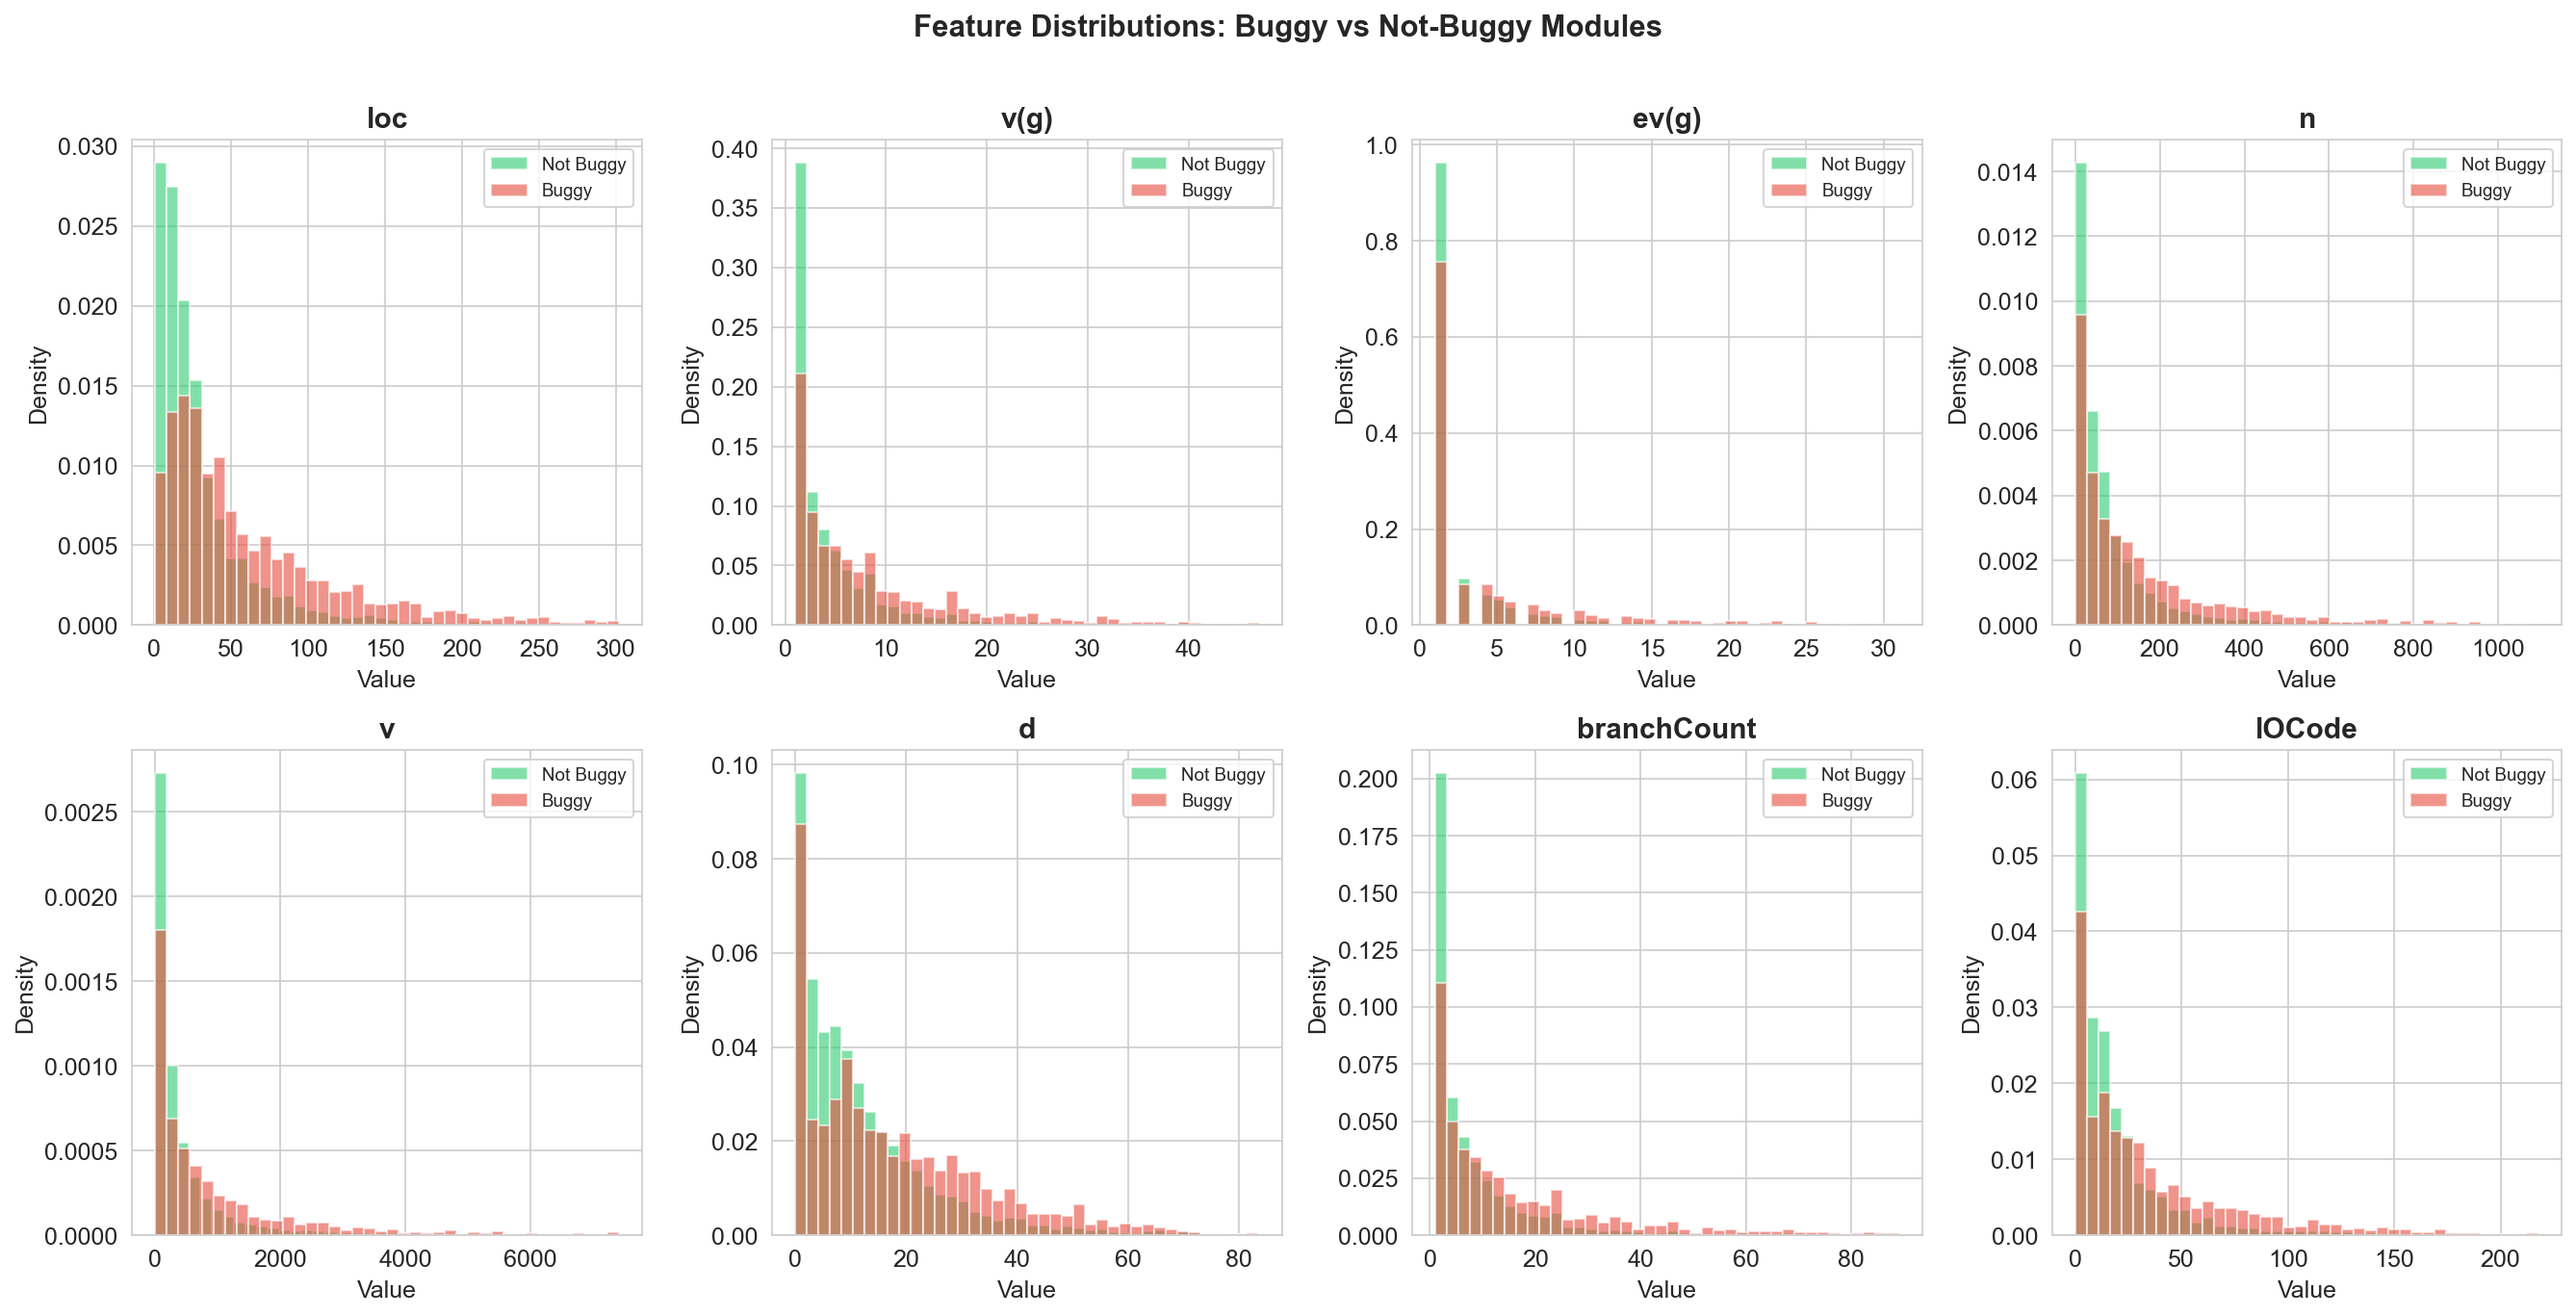
\includegraphics[width=0.95\linewidth]{02_feature_distributions.png}
\caption{Distributions of selected complexity metrics for defective and non-defective modules}
\label{fig:featdist}
\end{figure}

\begin{figure}[H]
\centering
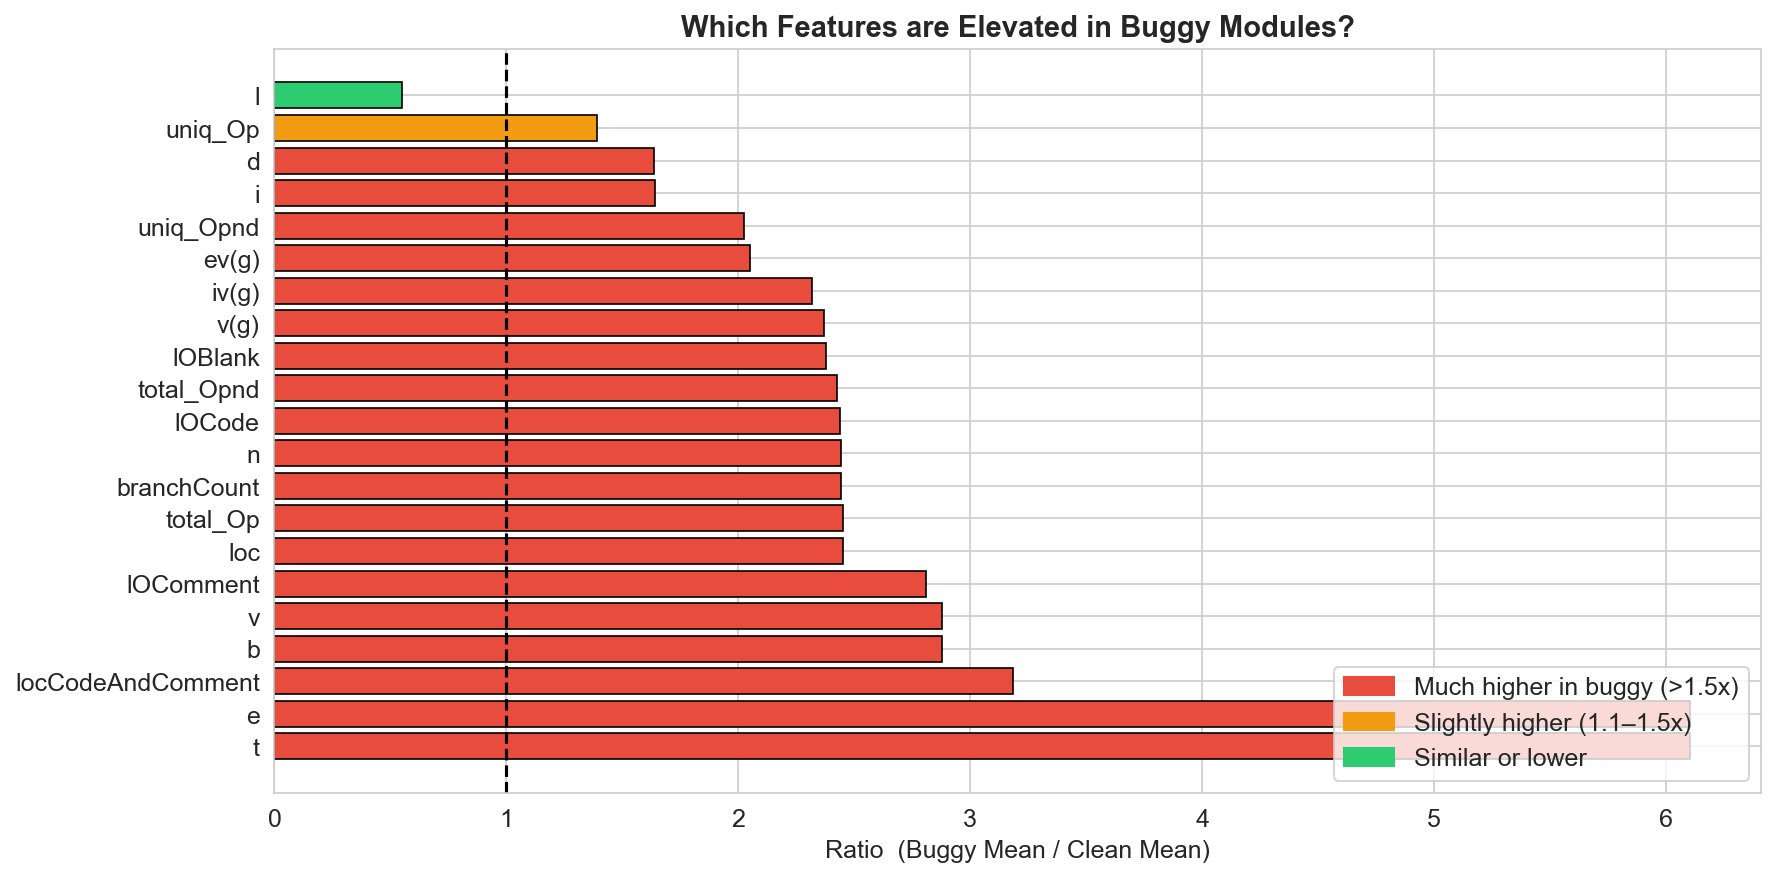
\includegraphics[width=0.95\linewidth]{03_feature_importance_ratio.png}
\caption{Ratio of mean feature value in defective modules to mean value in non-defective modules, for all 21 features}
\label{fig:featratio}
\end{figure}

Halstead effort and Halstead estimated time show the largest separation, with mean values 6.1 times higher in defective modules. This is consistent with the theoretical basis of these measures: both are derived quantities that compound program volume with program difficulty, and so amplify differences that the primitive counts express more modestly. Lines of code, cyclomatic complexity and branch count are approximately 2.4 times higher in defective modules, corroborating the long-standing empirical association between module size, control flow complexity and fault density reported since McCabe \cite{mccabe1976}.

That the signal is present in every feature but strong in none is the central difficulty of this dataset. No single metric separates the classes; the discriminative information is distributed across the feature set and is present in their interaction, which is the condition under which higher-capacity models are expected to have an advantage.

\subsection{Feature correlation}

Figure \ref{fig:corr} presents the correlation structure of the feature set.

\begin{figure}[H]
\centering
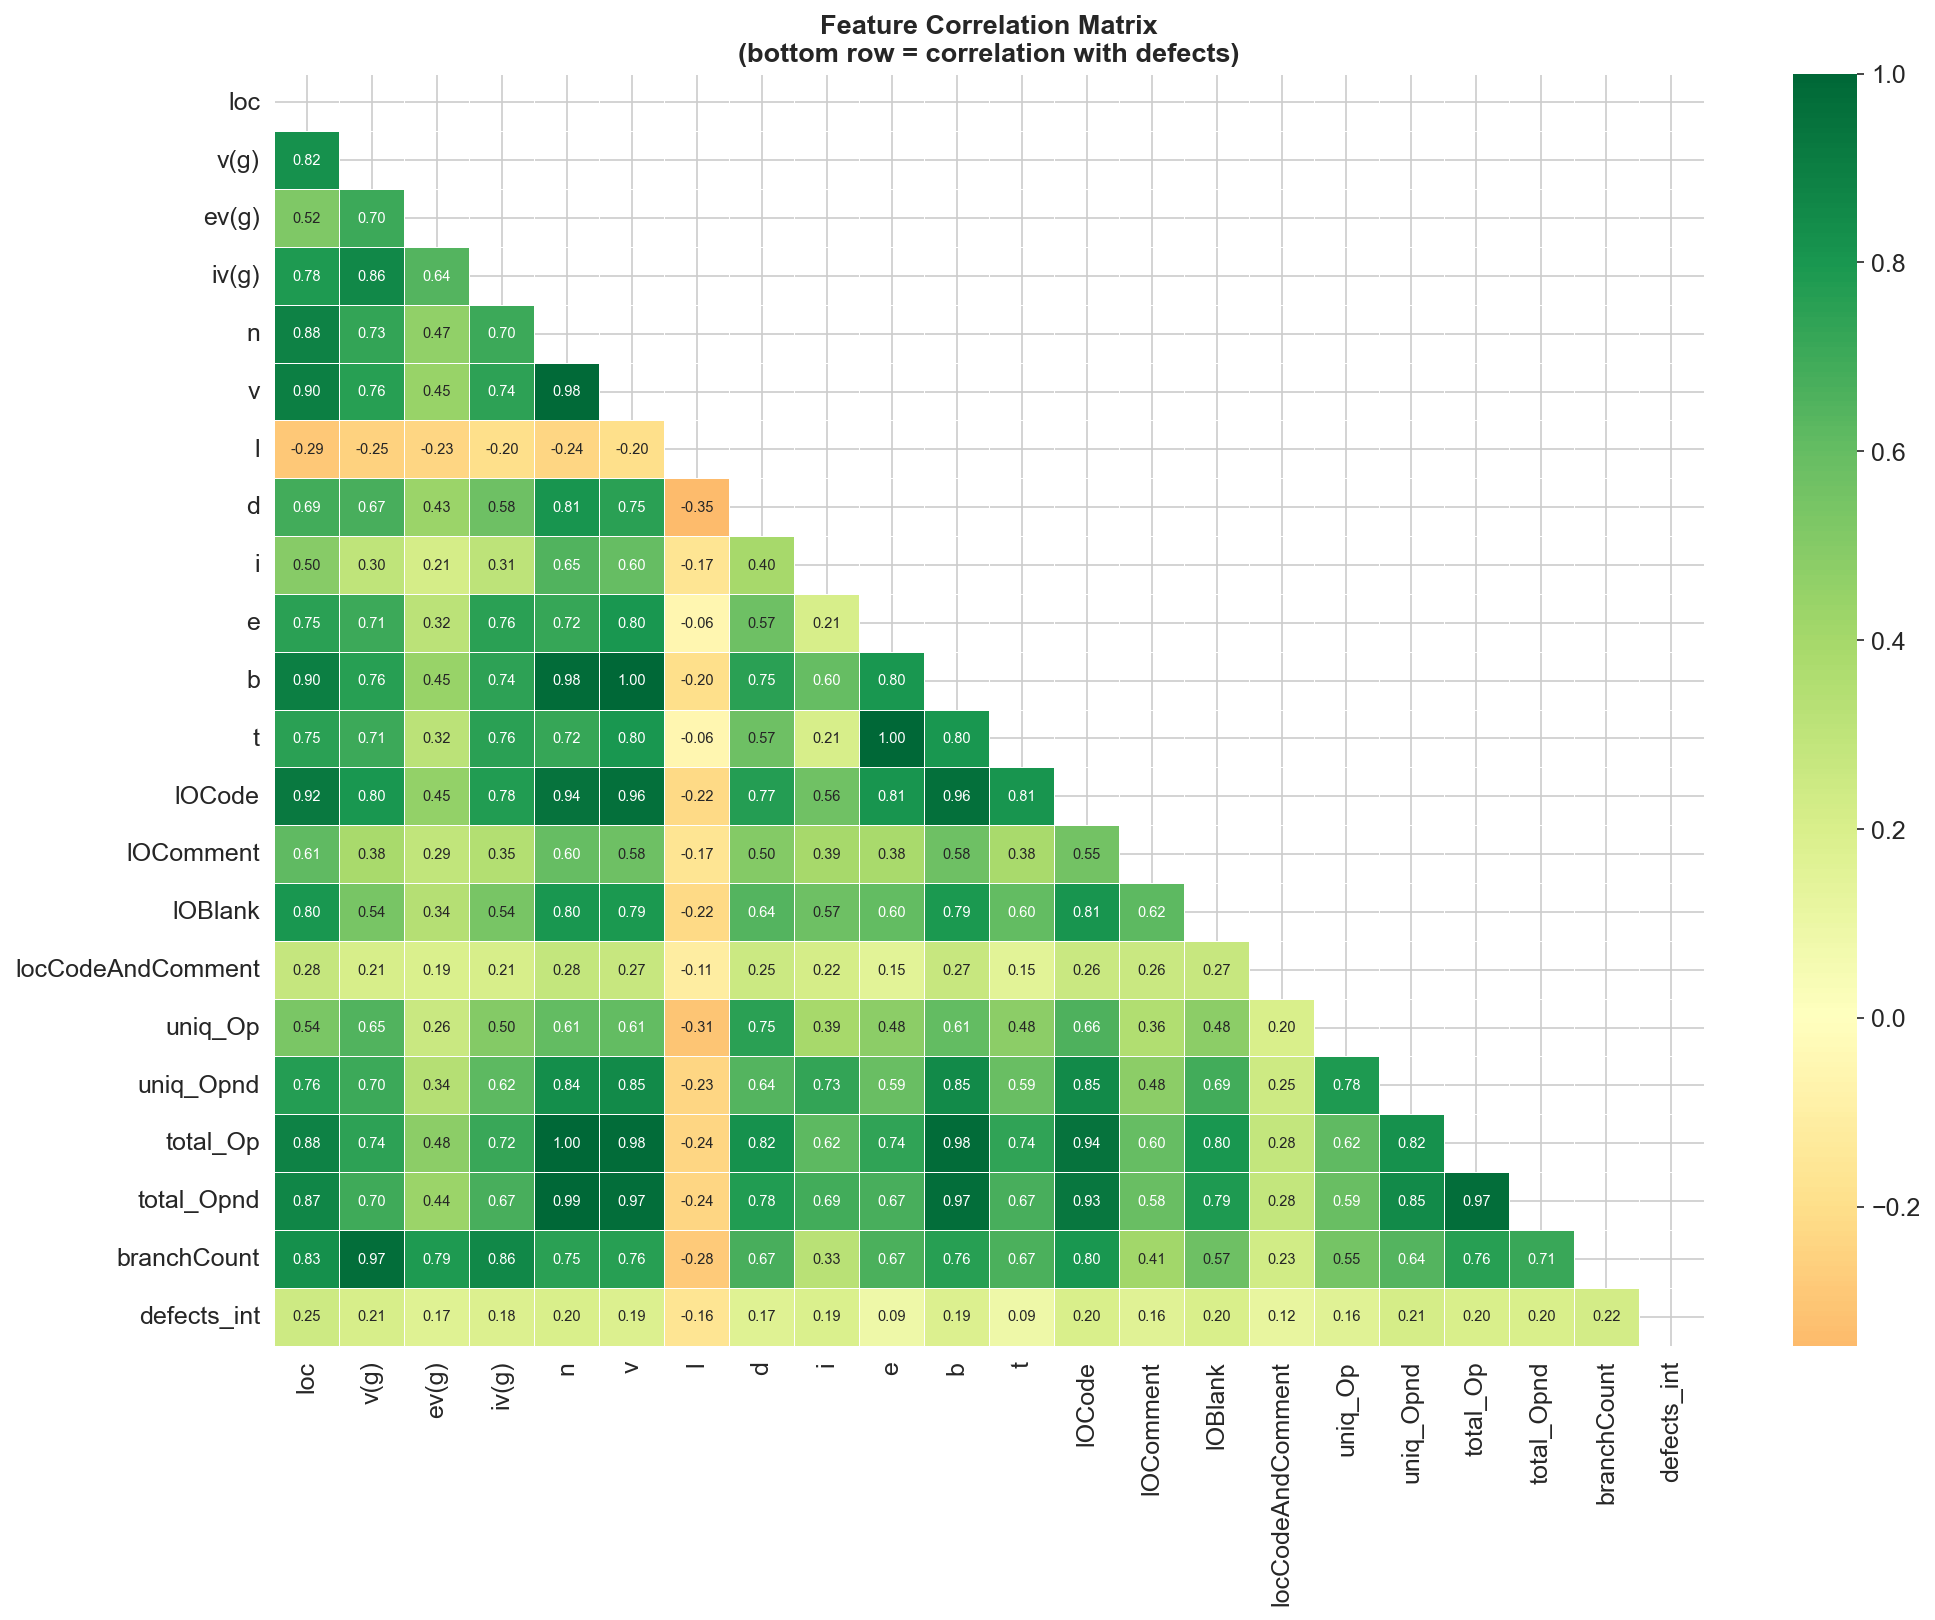
\includegraphics[width=0.88\linewidth]{04_correlation_heatmap.png}
\caption{Pearson correlation matrix of the 21 complexity metrics in the JM1 dataset}
\label{fig:corr}
\end{figure}

Strong positive correlations are evident within the Halstead family, which is expected given that these measures are algebraically derived from a common set of four primitive counts, and between lines of code, branch count and cyclomatic complexity, which measure related aspects of module size and control structure.

Neither feature selection nor dimensionality reduction was applied despite this redundancy. Two considerations support that decision. Random Forest is insensitive to correlated features by construction, since its random feature subsampling ensures that correlated predictors do not systematically exclude one another from the ensemble. The convolutional layers of the CNN-LSTM learn their own feature combinations, so imposing a fixed linear projection beforehand would constrain rather than assist the model. The one model materially disadvantaged by this correlation is Gaussian Naive Bayes, whose conditional independence assumption is violated; the consequence is visible in its results in Section 4.4.

\section{Preprocessing Results}

Preprocessing proceeded as specified in Section 3.4. Median imputation replaced 25 missing values. Winsorisation at the 99th percentile capped extreme values while retaining all 10,885 modules. The stratified partition produced a training set of 8,708 modules containing 1,685 defective instances and a test set of 2,177 modules containing 421 defective instances, both preserving the 4.2:1 ratio.

BorderlineSMOTE synthesised 5,338 defective instances in the training partition, producing 14,046 balanced training instances with 7,023 in each class, as shown in Figure \ref{fig:pipeline_smote} of Chapter 3. The test partition was left unmodified.

\section{Baseline Model Results}

Table \ref{tab:baseline} presents the performance of the four baseline configurations on the held-out test set of 2,177 modules containing 421 defective instances.

\begin{table}[H]
\centering
\caption{Baseline model results on the held-out test set}
\label{tab:baseline}
\tabfont
\begin{tabular}{L{32mm}C{14mm}C{14mm}C{14mm}C{14mm}C{14mm}C{18mm}}
\toprule
\textbf{Model} & \textbf{Acc.} & \textbf{Prec.} & \textbf{Recall} & \textbf{F1} & \textbf{AUC} & \textbf{Detected} \\
\midrule
RF, no SMOTE  & 0.8107 & 0.5280 & 0.2019 & 0.2921 & 0.7365 & 85 / 421 \\
RF + SMOTE    & 0.7653 & 0.4043 & 0.4513 & 0.4265 & 0.7350 & 190 / 421 \\
NB, no SMOTE  & 0.7901 & 0.4412 & 0.3207 & 0.3714 & 0.6788 & 135 / 421 \\
NB + SMOTE    & 0.7735 & 0.4037 & 0.3587 & 0.3799 & 0.6780 & 151 / 421 \\
\bottomrule
\end{tabular}
\end{table}

\subsection{The accuracy paradox}

Random Forest without SMOTE achieves the highest accuracy of any model in this study at 81.07 percent. It detects 85 of 421 defective modules, a recall of 0.202.

The comparison with the constant classifier is instructive. Predicting the majority class for every module yields 80.66 percent accuracy and zero detections. Random Forest without SMOTE therefore purchases 85 detections at a cost of 0.41 percentage points of accuracy. Judged on accuracy alone the two are near-indistinguishable, yet one is entirely useless and the other detects a fifth of the defects present. This is the clearest possible demonstration that accuracy cannot function as the evaluation criterion for this problem.

\subsection{The effect of BorderlineSMOTE}

Applying BorderlineSMOTE to the Random Forest training data raises recall from 0.202 to 0.451, increasing detections from 85 to 190, an improvement of 123.5 percent. Accuracy falls by 4.5 percentage points and precision from 0.528 to 0.404.

The mechanism is straightforward. In the unbalanced training set, the trees of the forest encounter defective instances rarely and the majority-vote aggregation is dominated by the majority class in most regions of the feature space. Synthesising minority instances along the class boundary shifts the learned decision boundary into territory previously assigned wholly to the majority class, capturing defective modules there at the cost of also capturing clean modules with similar metric profiles.

The trade-off is favourable under the cost asymmetry established in Section 3.6. The 105 additional detections are obtained at the cost of approximately 190 additional false alarms; given that a missed defect costs an order of magnitude more than a spurious review, the exchange is clearly worthwhile.

For Naive Bayes the same intervention produces a much smaller effect, raising recall from 0.321 to 0.359 and detections from 135 to 151. Naive Bayes fits a Gaussian to each feature within each class and is therefore sensitive to the location and spread of those distributions rather than to the density of instances. Synthetic instances generated along the boundary do not greatly alter the fitted class-conditional means and variances, so the decision boundary moves relatively little.

\subsection{The best baseline}

Random Forest with BorderlineSMOTE achieves the highest recall of 0.451 and the highest F1-score of 0.4265 among the traditional configurations, detecting 190 of 421 defective modules. It is adopted as the reference against which the deep learning results are compared. Figure \ref{fig:baselinecomp} presents the comparison across all four baseline configurations.

\begin{figure}[H]
\centering
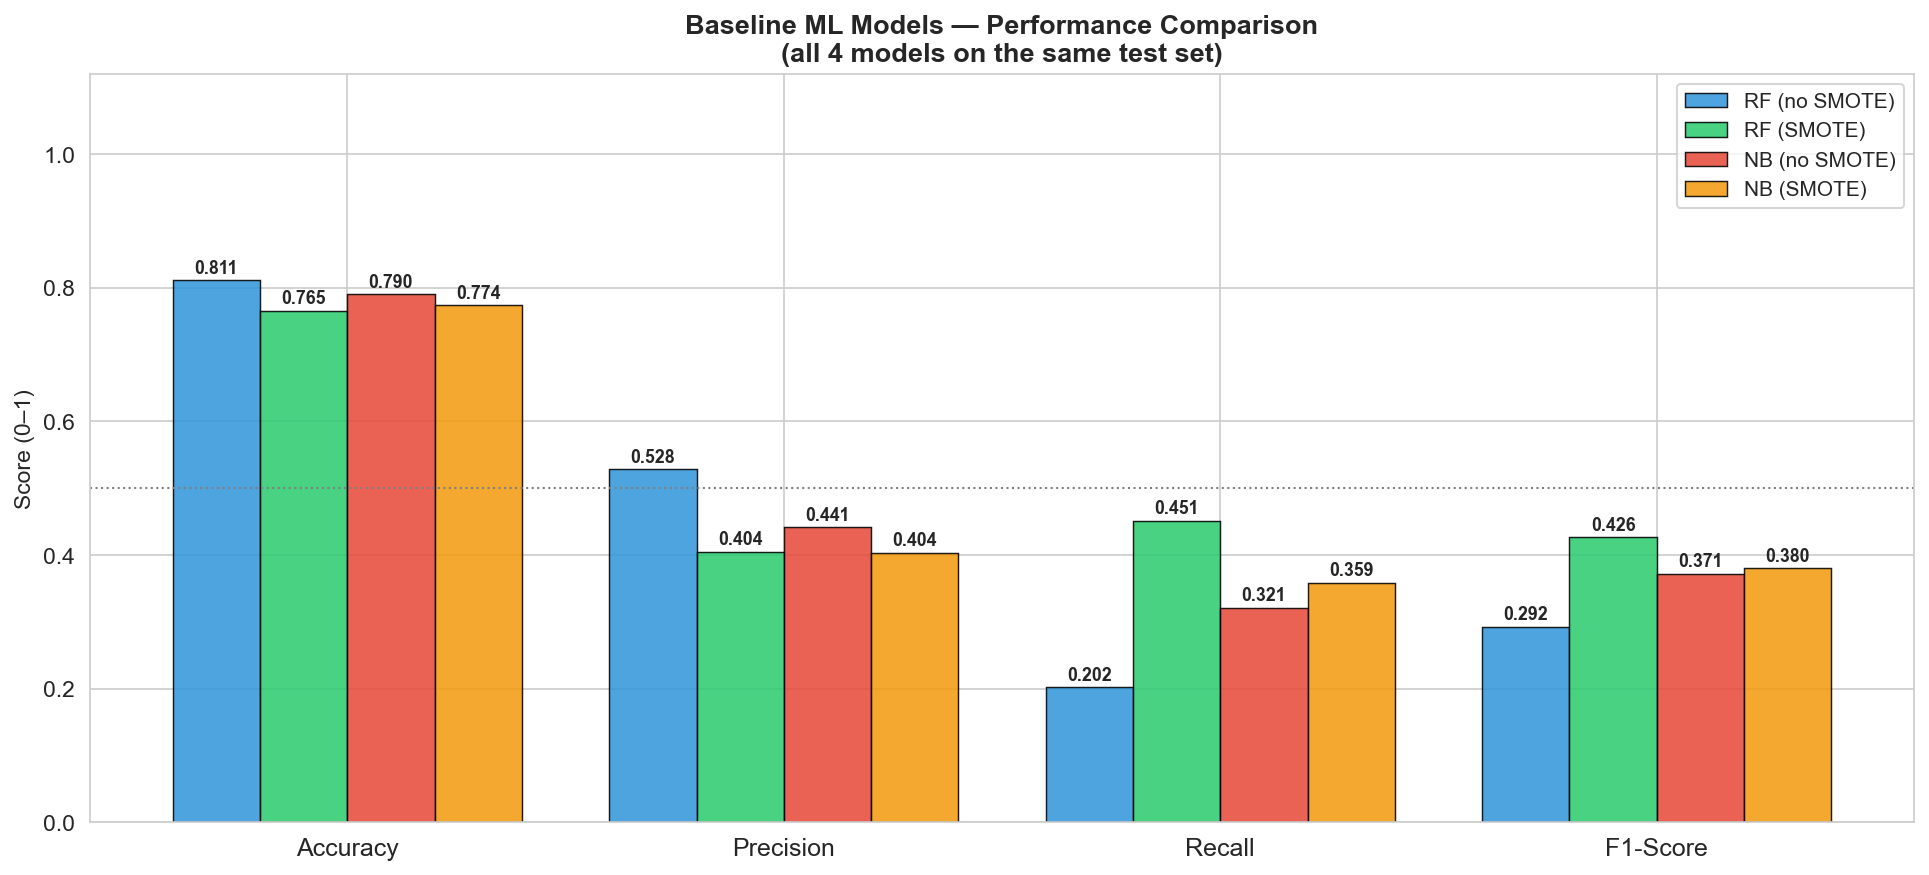
\includegraphics[width=0.92\linewidth]{11_baseline_comparison.png}
\caption{Comparison of the four baseline configurations across all evaluation metrics}
\label{fig:baselinecomp}
\end{figure}

Notably, Random Forest with SMOTE remains the strongest baseline despite ranking third of four on accuracy, which again confirms that the ordering induced by accuracy is not the ordering induced by practical utility. Confusion matrices for all four configurations are provided in Appendix A.

\section{Cross-Validation Results}

Table \ref{tab:cv} reports ten-fold stratified cross-validation for the two baseline models, conducted on the unbalanced data to characterise the stability of the estimates.

\begin{table}[H]
\centering
\caption{Ten-fold stratified cross-validation results for the baseline models}
\label{tab:cv}
\tabfont
\begin{tabular}{L{22mm}L{28mm}C{28mm}C{30mm}}
\toprule
\textbf{Model} & \textbf{Metric} & \textbf{Mean} & \textbf{Standard deviation} \\
\midrule
Random Forest & Accuracy  & 0.8168 & $\pm$ 0.0057 \\
Random Forest & Precision & 0.5816 & $\pm$ 0.0449 \\
Random Forest & Recall    & 0.1918 & $\pm$ 0.0315 \\
Random Forest & F1-score  & 0.2872 & $\pm$ 0.0378 \\
Random Forest & ROC-AUC   & 0.7618 & $\pm$ 0.0242 \\
\midrule
Naive Bayes   & Accuracy  & 0.7900 & $\pm$ 0.0084 \\
Naive Bayes   & Precision & 0.4385 & $\pm$ 0.0331 \\
Naive Bayes   & Recall    & 0.3091 & $\pm$ 0.0361 \\
Naive Bayes   & F1-score  & 0.3622 & $\pm$ 0.0350 \\
Naive Bayes   & ROC-AUC   & 0.6979 & $\pm$ 0.0322 \\
\bottomrule
\end{tabular}
\end{table}

The cross-validation means agree closely with the held-out test estimates reported in Table \ref{tab:baseline}. Random Forest recall is 0.1918 under cross-validation against 0.2019 on the test set, and F1-score 0.2872 against 0.2921; both test values lie within one standard deviation of the cross-validation mean. The corresponding Naive Bayes figures agree similarly. The held-out estimates are therefore representative rather than artefacts of a fortunate partition.

The standard deviations are small in absolute terms but their relative magnitude varies by metric. Accuracy varies by less than one percent of its mean, whereas recall varies by 16 percent of its mean. This asymmetry is itself a consequence of imbalance: accuracy is computed over 1,089 test instances per fold while recall is computed over approximately 210 defective instances, so the recall estimate is based on a fifth of the data and carries correspondingly greater sampling variance. Any single-split estimate of minority-class performance on an imbalanced dataset should be treated with this in mind.

\section{CNN-LSTM Results}

Table \ref{tab:cnnlstm} reports the CNN-LSTM under each of the three loss functions. All three configurations share an identical architecture, training data, optimiser family and evaluation protocol; they differ only in the loss function, so differences between rows are attributable to that factor alone.

\begin{table}[H]
\centering
\caption{CNN-LSTM results under three loss functions}
\label{tab:cnnlstm}
\tabfont
\begin{tabular}{L{38mm}C{14mm}C{14mm}C{14mm}C{14mm}C{14mm}C{17mm}}
\toprule
\textbf{Configuration} & \textbf{Acc.} & \textbf{Prec.} & \textbf{Recall} & \textbf{F1} & \textbf{AUC} & \textbf{Detected} \\
\midrule
CNN-LSTM, BCE    & 0.6647 & 0.3057 & 0.5772 & 0.3997 & 0.6808 & 243 / 421 \\
CNN-LSTM, FL     & 0.5581 & 0.2702 & 0.7553 & 0.3980 & 0.7001 & 318 / 421 \\
CNN-LSTM, CW-FL  & 0.4607 & 0.2412 & 0.8337 & 0.3742 & 0.6920 & 351 / 421 \\
\bottomrule
\end{tabular}
\end{table}

\subsection{The uncorrected deep learning baseline}

The CNN-LSTM trained with binary cross-entropy, without any imbalance-aware component in its objective, achieves a recall of 0.577 and detects 243 defective modules. This exceeds the best traditional baseline, Random Forest with SMOTE at 0.451 recall and 190 detections, by 53 additional detections.

This result is significant for the interpretation of the study as a whole, because it establishes that the advantage of the deep learning approach is not solely attributable to the loss function. The architecture itself extracts signal from the metric vector that the ensemble of axis-aligned decision trees does not, which is consistent with the observation in Section 4.2 that the discriminative information in this dataset resides in the interaction among features rather than in any individual feature. The convolutional layers are able to form composite features from combinations of adjacent metrics, and the LSTM aggregates these across the full vector.

The cost is a substantial reduction in accuracy, from 0.765 to 0.665, and in precision, from 0.404 to 0.306. The model flags considerably more modules than the Random Forest.

\subsection{The effect of Focal Loss}

Substituting Focal Loss with $\alpha = 0.75$ and $\gamma = 2.0$ for binary cross-entropy raises recall from 0.577 to 0.755, an increase of 17.8 percentage points, and detections from 243 to 318. ROC-AUC improves from 0.681 to 0.700, the highest value achieved by any deep learning configuration in this study.

The improvement in ROC-AUC merits attention because it is a threshold-independent measure. Recall can be increased trivially by lowering the decision threshold, which any model permits; an improvement in AUC indicates that the model has learned a better ranking of modules by defect probability, not merely that it has become more liberal in its predictions. Focal Loss has therefore improved what the model learned, not only how it decides.

The mechanism is that described in Section 2.4.2. Under binary cross-entropy the aggregate gradient is dominated by the large number of clean modules the model already classifies confidently. The factor $(1 - p_t)^{2}$ suppresses their contribution by up to two orders of magnitude, redirecting the gradient towards the modules near the decision boundary, which are disproportionately defective.

Precision falls from 0.306 to 0.270 and accuracy from 0.665 to 0.558. F1-score is essentially unchanged at 0.398, the gain in recall being offset almost exactly by the loss in precision.

\subsection{The effect of Class-Weighted Focal Loss}

The proposed Class-Weighted Focal Loss, which adds a class weight of $\rho = 4.2$ to the Focal Loss objective, raises recall further from 0.755 to 0.834 and detections from 318 to 351 of 421. This is the highest recall achieved by any code-metric model in this study.

Relative to the best traditional baseline, the improvement is from 190 to 351 detections, an increase of 84.7 percent. Expressed differently, Random Forest with SMOTE misses 231 of the 421 defective modules in the test set, while the CNN-LSTM with Class-Weighted Focal Loss misses 70.

The marginal contribution of the class weight, 7.9 percentage points of recall, is smaller than the marginal contribution of Focal Loss itself, 17.8 percentage points. This ordering is consistent with the account given in Section 3.5.5: the two components correct for different aspects of the imbalance, and the example-level focusing addresses the larger share of the problem in this dataset. The class weight supplies an additional, static correction that persists after focusing has suppressed the contribution of minority examples the model has learned to classify.

Accuracy falls to 0.461, below the 80.7 percent achievable by constant prediction, and precision to 0.241. F1-score declines to 0.374 from 0.398 under Focal Loss, indicating that the gain in recall no longer fully compensates for the loss in precision by the harmonic mean criterion.

These figures require interpretation rather than dismissal. The model flags 1,455 of the 2,177 test modules and among these are 351 of the 421 defects present. A review process operating on the model's output would examine two-thirds of the codebase and would encounter 83 percent of its defects. Whether this is an acceptable operating point depends on the cost of review relative to the cost of an escaped defect, a question that is properly a matter of engineering policy rather than of model selection. What the results establish is that the operating point is reachable, and that the models occupying the higher-precision region of the trade-off do not reach it.

Figure \ref{fig:roc} presents the ROC curves for all code-metric configurations.

\begin{figure}[H]
\centering
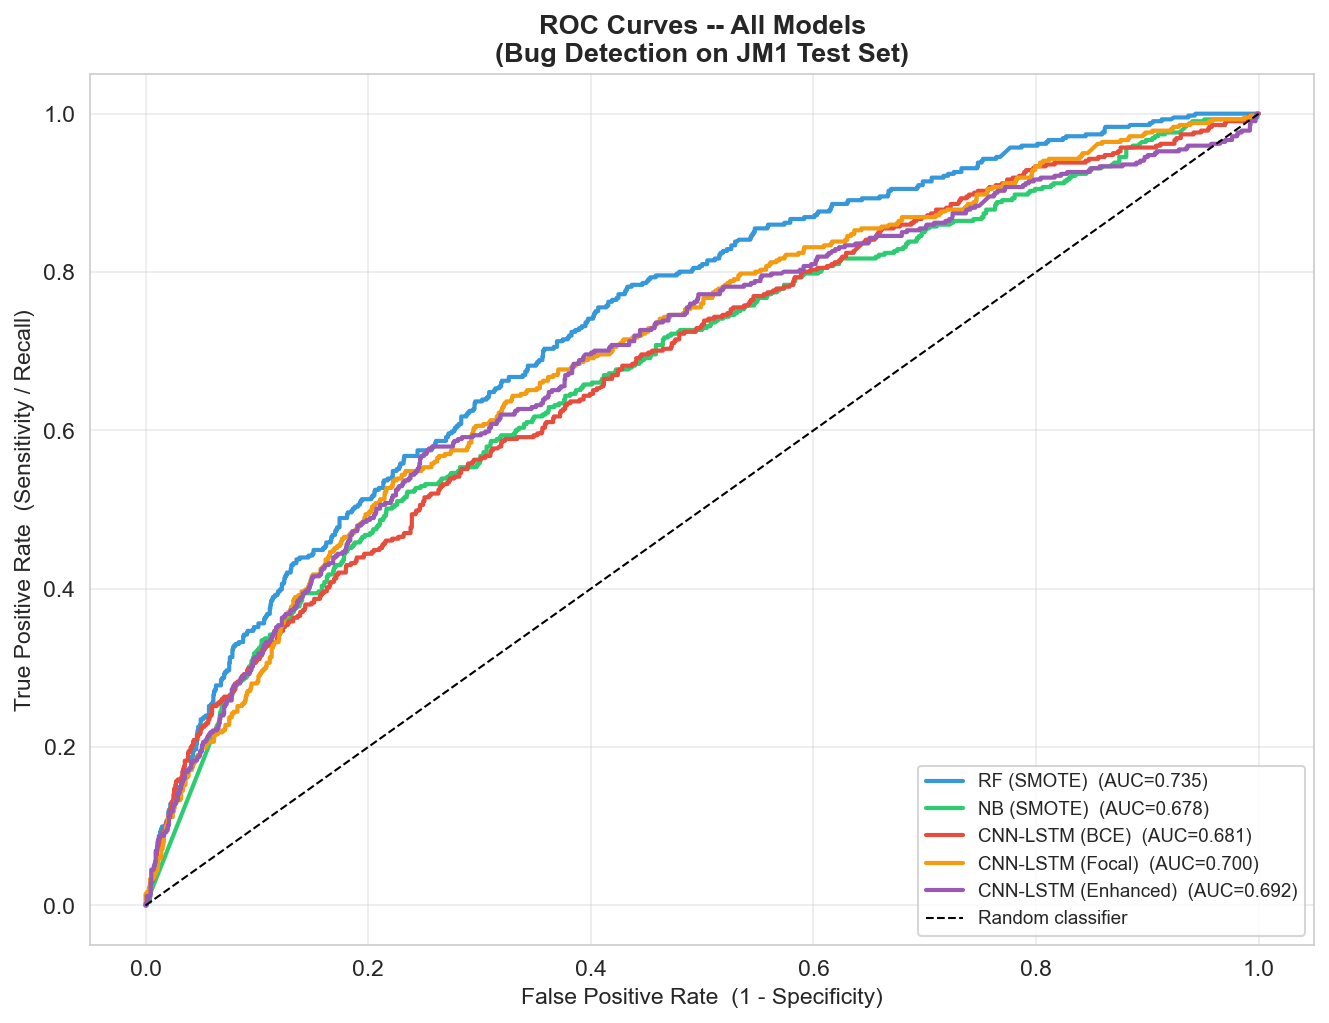
\includegraphics[width=0.9\linewidth]{18_roc_curves.png}
\caption{Receiver operating characteristic curves for all code-metric-based models}
\label{fig:roc}
\end{figure}

Training loss curves for the CNN-LSTM configurations are provided in Appendix A.

\section{DistilBERT Results}

DistilBERT fine-tuned on the bug report severity task achieved perfect classification on the 240-instance test set after four epochs. Table \ref{tab:bert} reports the results.

\begin{table}[H]
\centering
\caption{DistilBERT results on bug report severity classification}
\label{tab:bert}
\tabfont
\begin{tabular}{L{28mm}C{20mm}L{78mm}}
\toprule
\textbf{Metric} & \textbf{Value} & \textbf{Interpretation} \\
\midrule
Accuracy  & 1.0000 & All 240 test reports correctly classified \\
Precision & 1.0000 & No low-priority report classified as high-priority \\
Recall    & 1.0000 & No high-priority report missed \\
F1-score  & 1.0000 & Perfect balance of precision and recall \\
ROC-AUC   & 1.0000 & Complete separation of the two classes \\
\bottomrule
\end{tabular}
\end{table}

This result must be qualified carefully. Perfect classification indicates that the task, as constituted by this dataset, is separable by the model, and the reason it is separable is evident from the data. High-priority reports in this dataset contain lexical markers including crash, security vulnerability, memory leak and data loss; low-priority reports contain markers including cosmetic, typo, minor and alignment. These vocabularies do not overlap. A model equipped with pre-trained contextual embeddings requires very little adaptation to separate them.

The result therefore demonstrates that DistilBERT can learn a clean severity signal from a small labelled dataset with four epochs of fine-tuning on CPU hardware, which is a meaningful finding regarding the practicality of transformer fine-tuning under modest resources. It does not demonstrate that the model would achieve comparable performance on reports drawn from a live defect tracker, where severity labels are assigned inconsistently by many reporters and where a substantial proportion of reports do not signal their severity lexically at all. Published results on real Bugzilla data report F1-scores in the range 0.85 to 0.95 \cite{chen2022}, and that range is the appropriate expectation for a deployed system.

The training loss curve and confusion matrix are provided in Appendix A.

\section{Comprehensive Comparative Analysis}

Table \ref{tab:full} presents all seven code-metric configurations together with the DistilBERT result, ordered to show the progression from uncorrected traditional machine learning to fully corrected deep learning.

\begin{table}[H]
\centering
\caption{Complete comparison of all model configurations}
\label{tab:full}
\tabfont
\begin{tabular}{L{40mm}C{14mm}C{14mm}C{14mm}C{14mm}C{14mm}C{16mm}}
\toprule
\textbf{Model} & \textbf{Acc.} & \textbf{Prec.} & \textbf{Recall} & \textbf{F1} & \textbf{AUC} & \textbf{Detected} \\
\midrule
RF, no SMOTE     & 0.8107 & 0.5280 & 0.2019 & 0.2921 & 0.7365 & 85 \\
NB, no SMOTE     & 0.7901 & 0.4412 & 0.3207 & 0.3714 & 0.6788 & 135 \\
NB + SMOTE       & 0.7735 & 0.4037 & 0.3587 & 0.3799 & 0.6780 & 151 \\
RF + SMOTE       & 0.7653 & 0.4043 & 0.4513 & 0.4265 & 0.7350 & 190 \\
CNN-LSTM, BCE    & 0.6647 & 0.3057 & 0.5772 & 0.3997 & 0.6808 & 243 \\
CNN-LSTM, FL     & 0.5581 & 0.2702 & 0.7553 & 0.3980 & 0.7001 & 318 \\
\textbf{CNN-LSTM, CW-FL} & \textbf{0.4607} & \textbf{0.2412} & \textbf{0.8337} & \textbf{0.3742} & \textbf{0.6920} & \textbf{351} \\
\midrule
DistilBERT\textsuperscript{*} & 1.0000 & 1.0000 & 1.0000 & 1.0000 & 1.0000 & 120 / 120 \\
\bottomrule
\end{tabular}

\vspace{4pt}
{\footnotesize \textsuperscript{*}Evaluated on the bug report classification task, not on JM1. Not directly comparable to the rows above.}
\end{table}

Two patterns are evident in this table.

The first is a monotonic ordering. Reading down the seven code-metric rows, recall and detections increase strictly while accuracy and precision decrease strictly. There is no configuration that improves recall without cost, and no configuration that dominates another across all metrics. The choice among these models is unavoidably a choice of operating point on a trade-off, and presenting any single one as best without specifying the cost structure would be meaningless.

The second is that F1-score, the conventional summary metric for imbalanced classification, peaks at Random Forest with SMOTE at 0.4265 and declines thereafter. Ranking these models by F1-score would therefore select the traditional baseline over every deep learning configuration, including the one that detects 161 more defects. This is a limitation of F1-score rather than a finding about the models: the harmonic mean weights precision and recall equally, which encodes an assumption of symmetric error cost that Section 3.6 established to be false for this application. Where the cost asymmetry is as large as it is here, F1-score is the wrong summary and recall together with the absolute detection count is the appropriate criterion.

Figure \ref{fig:bugscaught} presents the detection counts directly and Figure \ref{fig:improvement} the improvement of each deep learning configuration over the best traditional baseline.

\begin{figure}[H]
\centering
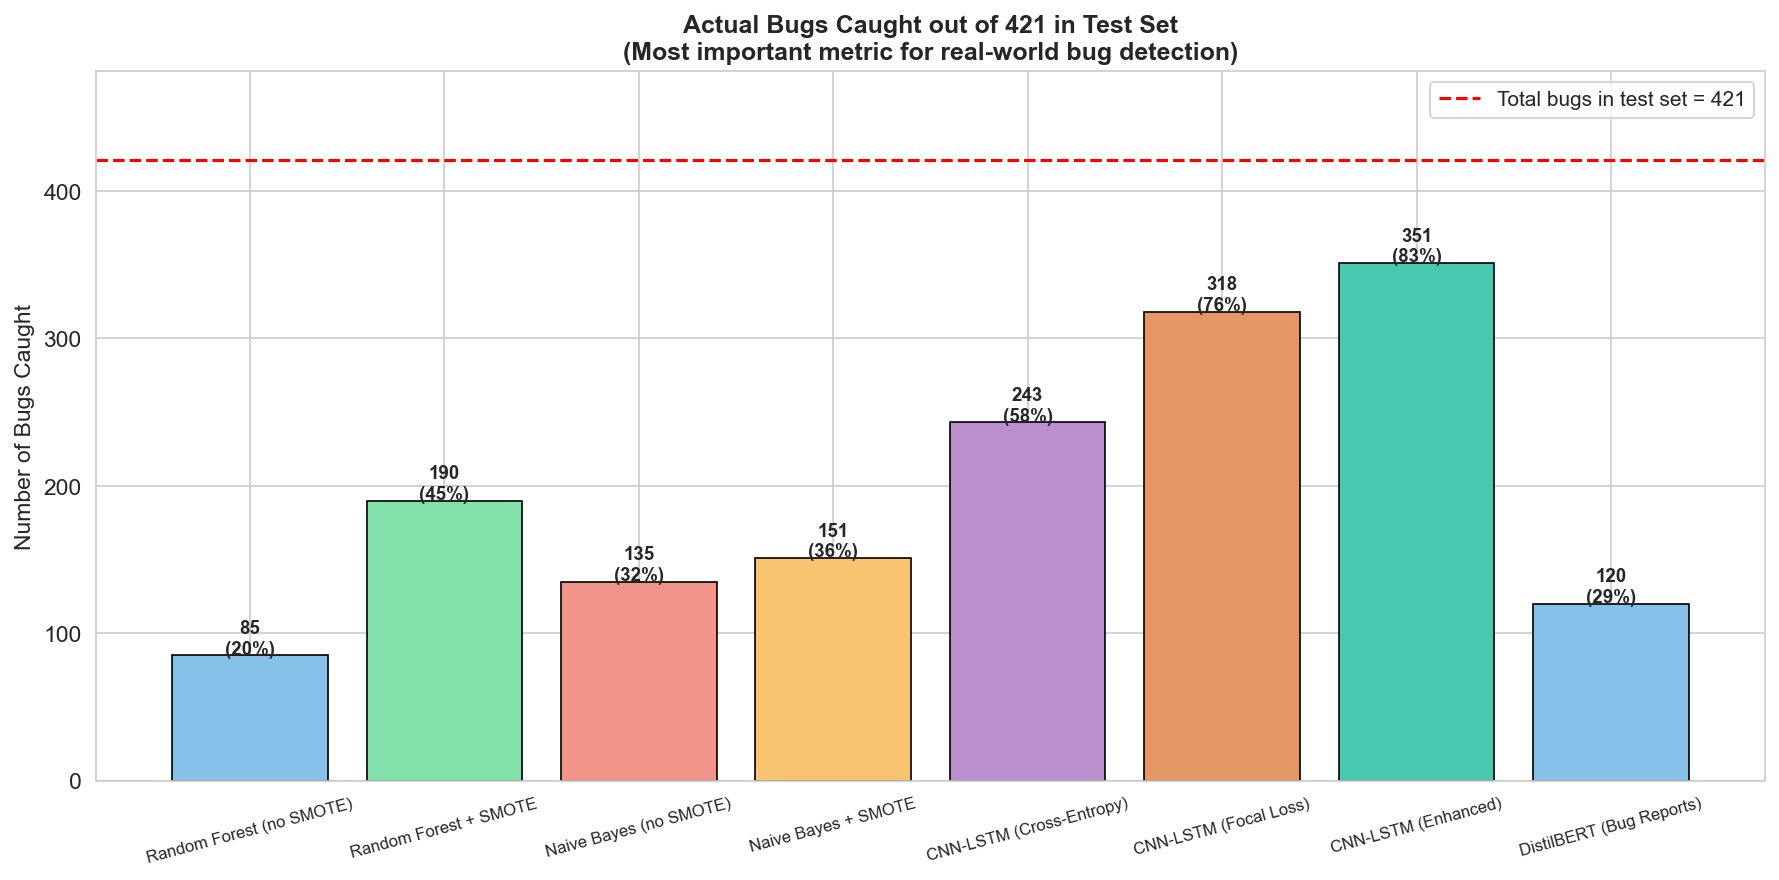
\includegraphics[width=0.95\linewidth]{21_bugs_caught.png}
\caption{Defective modules detected by each model out of the 421 present in the test set}
\label{fig:bugscaught}
\end{figure}

\begin{figure}[H]
\centering
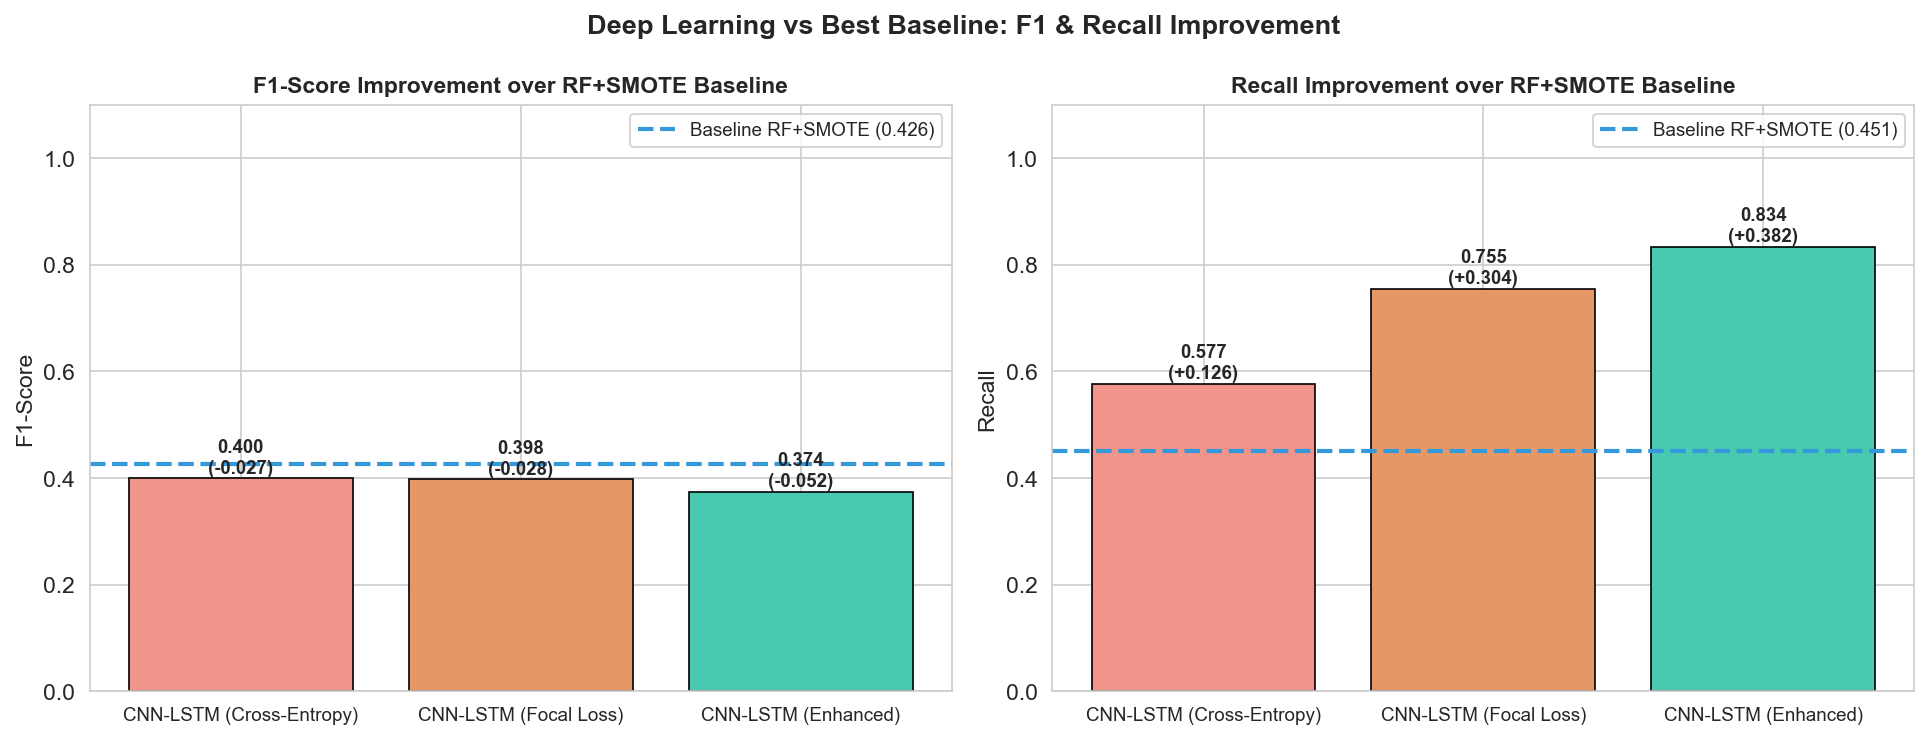
\includegraphics[width=0.9\linewidth]{20_improvement_over_baseline.png}
\caption{Recall and F1-score of the CNN-LSTM configurations relative to the Random Forest with SMOTE baseline}
\label{fig:improvement}
\end{figure}

\begin{figure}[H]
\centering
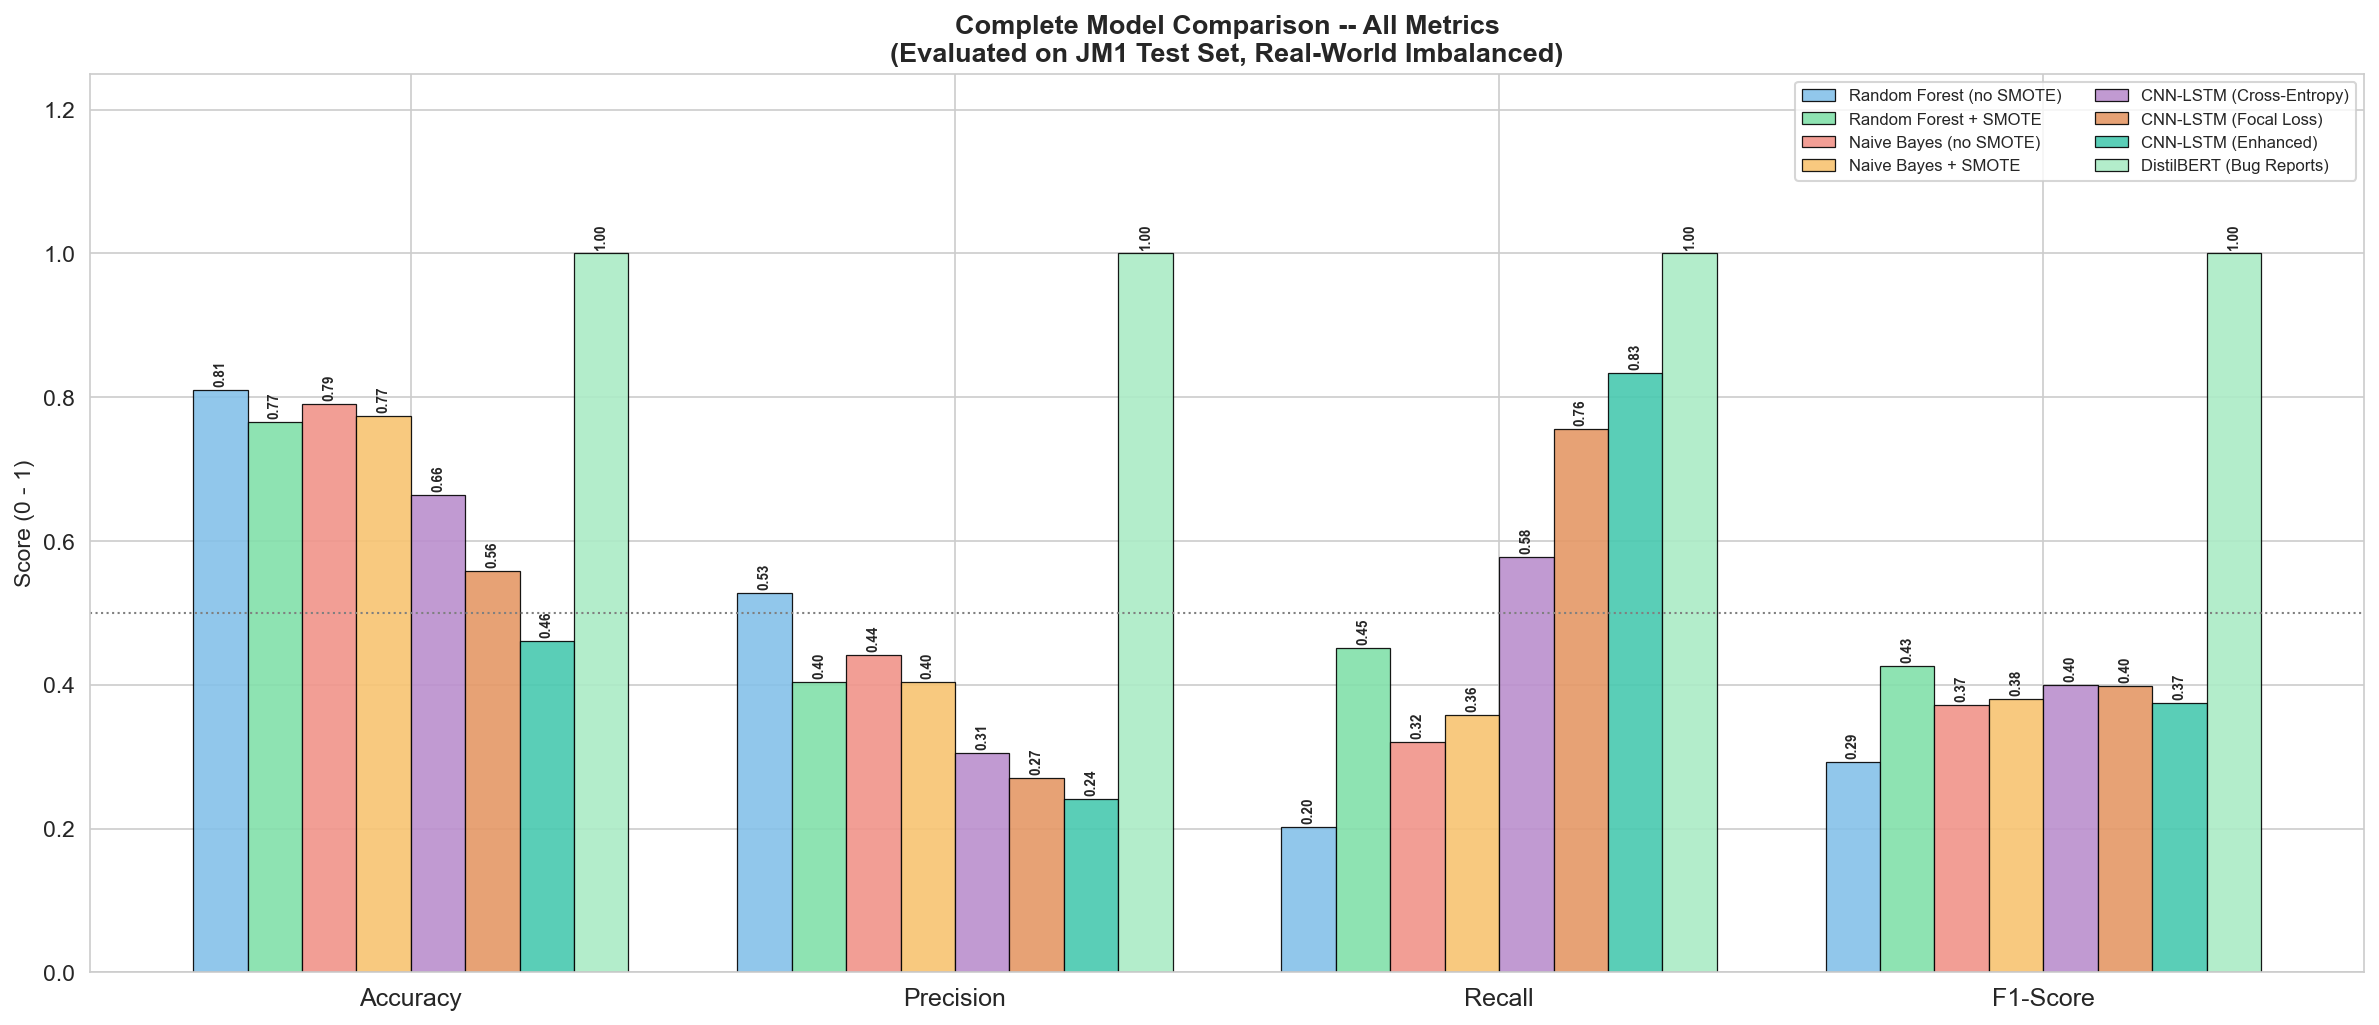
\includegraphics[width=0.95\linewidth]{19_final_comparison_bar.png}
\caption{Final comparison of all model configurations across the five evaluation metrics}
\label{fig:finalbar}
\end{figure}

\section{Findings}

The findings are stated below in the order of the research questions to which they correspond.

\subsection{Finding 1: Traditional machine learning against deep learning}

\textit{This finding addresses RQ1.}

The best traditional configuration, Random Forest with BorderlineSMOTE, achieved a recall of 0.451 and an F1-score of 0.4265, detecting 190 of 421 defective modules. The best deep learning configuration, the CNN-LSTM with Class-Weighted Focal Loss, achieved a recall of 0.834, detecting 351 of 421 modules, an improvement of 84.7 percent in the detection rate.

The advantage of the deep learning approach is not attributable solely to the loss function. The CNN-LSTM trained with ordinary binary cross-entropy, without any imbalance correction in its objective, already achieved a recall of 0.577 and 243 detections, exceeding every traditional configuration. The architecture and the objective therefore contribute separately, and both contribute positively.

Traditional models retain a clear advantage in precision, with Random Forest without SMOTE reaching 0.528 against 0.241 for the best deep configuration. Where review capacity is the binding constraint and the cost of an escaped defect is low, this advantage is material.

\subsection{Finding 2: The contribution of imbalance-aware training}

\textit{This finding addresses RQ2.}

The three CNN-LSTM configurations isolate the contribution of each component of imbalance correction, since they are identical in every respect but the loss function. Binary cross-entropy achieved a recall of 0.577. Adding example-level focusing through Focal Loss raised this to 0.755, a gain of 17.8 percentage points and 75 additional detections. Adding class-level weighting through the proposed Class-Weighted Focal Loss raised it further to 0.834, a gain of 7.9 percentage points and 33 additional detections.

Both components therefore contribute, and their contributions are additive in direction though unequal in magnitude. The larger contribution comes from example-level focusing, consistent with the argument in Section 3.5.5 that it is the adaptive component and addresses the dominant share of the problem in this dataset.

Focal Loss additionally improved ROC-AUC from 0.681 to 0.700, establishing that the improvement reflects better learned discrimination rather than merely a more liberal decision threshold.

DistilBERT achieved perfect classification on the bug report task, subject to the qualification stated in Section 4.7 regarding the lexical separability of the constructed dataset.

\subsection{Finding 3: The impact of class imbalance}

\textit{This finding addresses RQ3.}

Class imbalance is confirmed as the dominant factor governing performance on this dataset. Without any correction, Random Forest detected 85 of 421 defective modules, a recall of 0.202, while achieving 81.07 percent accuracy, a figure that a constant prediction of the majority class attains at 80.66 percent with zero detections.

Data-level correction through BorderlineSMOTE raised Random Forest recall by 123.5 percent, from 0.202 to 0.451. Algorithm-level correction through Focal Loss raised CNN-LSTM recall by 30.8 percent, from 0.577 to 0.755. Applied in combination, with BorderlineSMOTE on the training data and Class-Weighted Focal Loss as the objective, recall reached 0.834.

The two forms of correction are therefore complementary and not substitutable. They intervene at different points in the learning pipeline, one modifying the training distribution and the other the objective function, and the effect of applying both exceeds the effect of either alone.

The cross-validation results in Section 4.5 further establish that imbalance affects the reliability of measurement as well as the performance of models: the standard deviation of recall across folds was 16 percent of its mean, against under one percent for accuracy, because recall is estimated from only the minority instances in each fold.

\subsection{Finding 4: Model selection for scalable defect detection}

\textit{This finding addresses RQ4.}

No configuration dominates across all metrics, and model selection is therefore determined by the cost structure of the application rather than by a single performance figure.

Where the cost of an escaped defect substantially exceeds the cost of reviewing a clean module, which is the condition in safety-critical and security-sensitive software, the CNN-LSTM with Class-Weighted Focal Loss is the appropriate selection. It detects 351 of 421 defects, missing 70, and flags 1,455 of 2,177 modules for review.

Where review capacity is limited and false alarms carry a high cost in developer confidence, Random Forest with BorderlineSMOTE is the appropriate selection. It detects 190 defects, missing 231, but its higher precision of 0.404 means that a larger proportion of the modules it flags repay the effort of examining them.

For bug report severity classification, DistilBERT is the appropriate selection, subject to validation on data from the target defect tracker before deployment.

The two tasks are complementary rather than competing. The CNN-LSTM operates on code before defects are reported and identifies where they are likely to be; DistilBERT operates on reports after defects are discovered and determines how they should be prioritised. Deployed together they address consecutive stages of the same quality assurance process.

\section{Summary}

The results establish that class imbalance is the dominant obstacle to effective defect prediction on the JM1 dataset, that both data-level and algorithm-level correction produce substantial improvements in detection, that their combination outperforms either alone, and that the hybrid CNN-LSTM architecture extracts signal from the complexity metrics beyond what the traditional baselines obtain. The proposed Class-Weighted Focal Loss achieved the highest recall of any code-metric configuration at 0.834, detecting 351 of 421 defective modules against 190 for the best traditional baseline. Every improvement in recall was obtained at a measured cost in precision, and the resulting trade-off is characterised explicitly. The following chapter discusses these findings and draws conclusions.

\clearpage

%% ================================================================
%%  CHAPTER 5 -- DISCUSSION AND CONCLUSION
%% ================================================================
\chapter{Discussion and Conclusion}

\section{Introduction}

This chapter interprets the results reported in Chapter 4, draws conclusions from them, states the limitations that qualify those conclusions, and recommends directions for further research. Section 5.2 summarises the findings and their implications. Section 5.3 discusses the results in relation to the literature reviewed in Chapter 2. Section 5.4 states the specific conclusions the evidence supports. Section 5.5 sets out the limitations. Section 5.6 gives recommendations for further research and Section 5.7 concludes.

\section{Summary of Findings}

Six findings emerge from the study.

\textbf{First, class imbalance is the dominant obstacle in software defect prediction, and accuracy is an actively misleading metric in its presence.} Random Forest without correction achieved 81.07 percent accuracy while detecting 85 of 421 defective modules. A model predicting the majority class for every input achieves 80.66 percent accuracy and detects none. The 0.41 percentage point difference between these two models on the accuracy metric conceals the entire difference in their utility. Any evaluation of defect prediction that reports accuracy as its headline figure should be regarded as uninformative.

\textbf{Second, data-level correction produces substantial improvement but leaves most defects undetected.} BorderlineSMOTE raised Random Forest recall from 0.202 to 0.451, an improvement of 123.5 percent and 105 additional detections. This is a large gain in relative terms. It nonetheless leaves 231 of 421 defective modules undetected, which is to say that the best traditional configuration in this study misses more defects than it finds.

\textbf{Third, the deep learning architecture extracts signal that the traditional models do not, independently of the loss function.} The CNN-LSTM trained with ordinary binary cross-entropy achieved a recall of 0.577 and 243 detections, exceeding every traditional configuration including those with SMOTE applied. Since this configuration incorporates no imbalance-aware component in its objective, the improvement is attributable to the representational capacity of the architecture. This is consistent with the exploratory finding that discriminative information in this dataset is distributed across the feature set and resides in the interaction among metrics rather than in any single metric.

\textbf{Fourth, algorithm-level correction produces gains beyond those available from data-level correction alone, and the two components of the proposed loss contribute separately.} Focal Loss raised recall from 0.577 to 0.755, a gain of 17.8 percentage points. The addition of the class weight in the proposed Class-Weighted Focal Loss raised it further to 0.834, a gain of 7.9 percentage points. That Focal Loss also raised ROC-AUC from 0.681 to 0.700 establishes that it improved the model's learned ranking of modules by defect probability rather than merely shifting its decision threshold.

\textbf{Fifth, the combined effect is an 84.7 percent improvement in detection rate over the best traditional baseline.} The CNN-LSTM with Class-Weighted Focal Loss detected 351 of 421 defective modules against 190 for Random Forest with SMOTE. Expressed in terms of failure, the traditional baseline misses 231 defects and the proposed configuration misses 70.

\textbf{Sixth, every gain in recall was purchased at a measured cost in precision, and no configuration dominates.} Precision declined monotonically from 0.528 for the most conservative configuration to 0.241 for the most aggressive. The choice among these models is therefore a choice of operating point, determined by the relative cost of an escaped defect and a wasted review in the deploying organisation.

\section{Discussion}

\subsection{The precision-recall trade-off and its practical interpretation}

The most consequential aspect of the results is the trade-off exposed in Table \ref{tab:full}, in which recall rises monotonically and precision falls monotonically across the seven code-metric configurations. It is worth stating plainly what the extreme configuration means in operational terms. The CNN-LSTM with Class-Weighted Focal Loss flags 1,455 of the 2,177 test modules, approximately two-thirds of the codebase, and among those flagged are 351 of the 421 defects present.

Whether this is useful depends entirely on what the alternative is. If the alternative is reviewing the entire codebase, the model has reduced the review burden by a third while retaining 83 percent of the defects. If the alternative is reviewing nothing, the model has identified a two-thirds subset within which the great majority of defects lie. If the alternative is a traditional model flagging a much smaller set, then the comparison is between 351 detections at a review cost of 1,455 modules and 190 detections at a review cost of 470 modules, and the correct choice depends on the marginal cost of review against the marginal cost of an escaped defect.

This last comparison is instructive. The traditional model finds 190 defects per 470 modules reviewed, a yield of 0.40 defects per module. The proposed model finds 351 per 1,455, a yield of 0.24. The proposed model is therefore less efficient per unit of review effort, but achieves a level of coverage that the traditional model cannot reach at any threshold. Where coverage is the binding requirement, as in safety-critical certification, efficiency is secondary. Where review capacity is the binding constraint, efficiency dominates.

The contribution of this study is not that one operating point is correct but that the frontier extends further than the traditional models reach, and that the extension is obtained by a specific and reproducible modification to the training objective.

\subsection{The inadequacy of F1-score as a summary metric}

A result that deserves emphasis because it runs against convention is that F1-score, the standard summary metric for imbalanced classification, peaks at Random Forest with SMOTE at 0.4265 and declines across every deep learning configuration. Ranking the models by F1-score would select the traditional baseline over the configuration that detects 161 additional defects.

This is a property of the metric rather than a finding about the models. The harmonic mean weights precision and recall equally, which is appropriate only when the two error types carry comparable cost. Section 3.6 established, following Boehm \cite{boehm1981}, that in defect prediction they do not: a defect escaping to production costs an order of magnitude more than a spurious review. F1-score encodes an assumption that the application violates.

The implication for the field is that studies reporting F1-score as the primary criterion for defect prediction may be systematically selecting models that are conservative relative to what the cost structure warrants. A cost-weighted metric such as $F_\beta$ with $\beta > 1$, or direct reporting of detections against review burden as in Table \ref{tab:full}, would better reflect the decision the model is intended to support.

\subsection{Relation to the reviewed literature}

The finding that Random Forest is a strong baseline is consistent with Menzies and colleagues \cite{menzies2010}, who argued that simple models on well-prepared features are difficult to improve upon. This study qualifies rather than contradicts that position. Random Forest with SMOTE was indeed the strongest configuration by F1-score, and no deep learning configuration surpassed it on that metric. But the deep learning configurations reached recall values that Random Forest did not attain, which suggests the ceiling Menzies identified is a ceiling on the precision-recall product rather than on recall as such.

The finding that Focal Loss transfers effectively from computer vision to software defect prediction extends Lin and colleagues \cite{lin2017} into a domain they did not consider. The transfer is not automatic, since the imbalance in dense object detection is far more extreme, at ratios of roughly 1000:1 against the 4.2:1 here, and the examples are images rather than metric vectors. That the technique nonetheless produced a 30.8 percent relative improvement in recall indicates that the mechanism it exploits, the domination of the aggregate gradient by easy majority examples, is general rather than specific to vision.

The proposed extension of Focal Loss with an explicit class weight set to the observed imbalance ratio addresses the gap identified in Section 2.7. Lin and colleagues used $\alpha$ as a class weighting factor within the focal term; the present study additionally applies a multiplicative class weight outside it. The empirical result, a further 7.9 percentage point gain in recall, supports the argument that the adaptive example-level term and the static class-level term correct for distinguishable aspects of the problem.

The DistilBERT result is consistent with Chen and colleagues \cite{chen2022} in direction but not in magnitude, and the difference is attributable to the data rather than the model, as discussed in Section 4.7.

\subsection{Why the deep architecture succeeded without loss correction}

An aspect of the results that warrants specific comment is that the CNN-LSTM trained with binary cross-entropy outperformed Random Forest with SMOTE in recall, 0.577 against 0.451, despite having no imbalance correction in its objective while the Random Forest had its training data explicitly rebalanced.

The exploratory analysis in Section 4.2 offers an explanation. Twenty of 21 features showed elevated means in defective modules, but none separated the classes cleanly, and the features were strongly intercorrelated. This is precisely the condition under which a model restricted to axis-aligned splits on individual features is at a disadvantage relative to a model that can form arbitrary combinations of them. Each decision tree in the forest partitions the space by thresholding one feature at a time; the convolutional layers of the CNN-LSTM learn weighted combinations of adjacent metrics and the LSTM aggregates these across the vector.

The implication is that architecture and objective are separable levers, and that a study varying only one of them would attribute to it effects properly belonging to both. The factorial design described in Section 3.2 was adopted specifically to avoid that confound.

\section{Conclusions Drawn by Results}

The evidence supports the following specific conclusions.

\textbf{Conclusion 1.} Accuracy is not a valid criterion for evaluating software defect prediction models on imbalanced data, and its use as a headline metric conceals rather than reveals model utility. The demonstration is direct: a difference of 0.41 percentage points in accuracy separated a model detecting 85 defects from one detecting none.

\textbf{Conclusion 2.} Data-level and algorithm-level imbalance correction are complementary rather than substitutable interventions. They act at different points in the learning pipeline, one on the training distribution and one on the objective function, and the effect of applying both exceeds the effect of either alone. Studies applying only one form of correction understate the improvement available.

\textbf{Conclusion 3.} The proposed Class-Weighted Focal Loss is an effective objective for minority-class detection in software defect prediction. Applied to a hybrid CNN-LSTM architecture it raised recall to 0.834 and detections to 351 of 421, against 0.451 and 190 for the best traditional configuration, an improvement of 84.7 percent in detection rate.

\textbf{Conclusion 4.} The advantage of the deep learning approach in this domain arises from both the architecture and the objective, and these contribute independently. The architecture alone, trained with an uncorrected objective, exceeded every traditional configuration in recall; the objective added a further 25.7 percentage points on top of that.

\textbf{Conclusion 5.} F1-score is an inappropriate primary criterion for model selection in software defect prediction, because it presumes symmetric error costs that the application does not exhibit. Selection should be made on recall together with an explicit accounting of the review burden induced.

\textbf{Conclusion 6.} Transformer models fine-tuned on modest hardware are effective for bug report severity classification where the severity signal is lexically expressed, though performance on data from live defect trackers should be expected to be lower and must be validated before deployment.

\section{Limitations}

The conclusions above are qualified by the following limitations.

\textbf{Single-dataset evaluation.} All defect prediction results derive from JM1. The dataset is a recognised benchmark and its imbalance ratio is representative, but a single dataset cannot establish generality. The relationships between complexity metrics and defectiveness observed here may differ in other languages, domains and organisations, and no cross-project validation was performed.

\textbf{Constructed bug report dataset.} The DistilBERT experiment used a dataset built from structural templates rather than exported from a live tracker. The perfect classification result reflects the lexical separability of that dataset, and Section 4.7 states the appropriate expectation for real data. This limitation constrains the strength of Conclusion 6.

\textbf{No cross-validation of the deep learning models.} Ten-fold cross-validation was applied only to the baselines. Deep learning results rest on a single held-out evaluation, and the cross-validation results in Section 4.5 showed that recall estimates on this dataset carry a standard deviation of approximately 16 percent of their mean. The deep learning recall figures should be read with a comparable uncertainty, which was not directly measured.

\textbf{CPU-only training.} The absence of accelerator hardware restricted training epochs and hyperparameter exploration. The values $\alpha = 0.75$, $\gamma = 2.0$ and $\rho = 4.2$ were selected on principled grounds rather than by systematic search, and it is unknown whether a search would identify better values.

\textbf{Static feature representation.} The 21 metrics describe a module at a single point in time. Process metrics, including code churn, developer experience, and prior defect history in the same module, are known predictors of defectiveness and were unavailable in the JM1 distribution.

\textbf{Absence of explainability analysis.} The models produce predictions without rationale. A developer told that a module is probably defective, without any indication of which characteristics of the module drove the prediction, receives limited actionable guidance.

\section{Recommendations for Further Research}

Six directions are recommended, ordered by their proximity to the present work.

\textbf{First, cross-dataset and cross-project validation.} The evaluation should be extended to KC1 and PC1 from the PROMISE repository, which share the JM1 feature schema and can therefore be incorporated with minimal modification to the pipeline. Beyond within-dataset evaluation, cross-project validation, training on one project and testing on another, would establish whether the Class-Weighted Focal Loss advantage persists under distribution shift. This is the single most important extension, since it directly addresses the principal limitation of the present study.

\textbf{Second, systematic hyperparameter search on the loss function.} The values of $\alpha$, $\gamma$ and $\rho$ were fixed on principled rather than empirical grounds. A grid or Bayesian search over these three parameters, on hardware permitting repeated training, would establish the sensitivity of the result to their choice and identify whether the observed improvement can be extended. It would also determine whether the optimal $\rho$ coincides with the imbalance ratio, as the construction assumes, or diverges from it.

\textbf{Third, cost-sensitive evaluation.} Given the finding that F1-score misranks models under asymmetric error cost, further work should evaluate using explicitly cost-weighted criteria, for instance $F_\beta$ with $\beta$ calibrated to an estimated cost ratio, or expected cost curves. This would place model selection on a principled footing rather than requiring the qualitative judgement Section 4.9.4 falls back on.

\textbf{Fourth, evaluation on live bug report data.} The DistilBERT result should be reproduced on an export from a real defect tracker, such as the Eclipse or Mozilla Bugzilla archives, with their authentic label noise and severity ambiguity. This would establish the practical ceiling for the bug triage component and would test whether the qualification stated in Section 4.7 is correct.

\textbf{Fifth, integration of explainability methods.} Applying SHAP or LIME to the CNN-LSTM predictions would produce feature-level attributions for individual modules, converting a bare prediction into actionable guidance. This addresses a limitation that is practical rather than statistical: a model that cannot explain itself will not be trusted by the developers expected to act on it, regardless of its measured recall.

\textbf{Sixth, richer feature representations.} Two extensions are indicated. Process metrics, including code churn and prior defect history, should be incorporated where available, since the literature establishes them as strong predictors complementary to static complexity. Beyond this, graph neural networks applied to abstract syntax trees would capture structural relationships in the code that a flat metric vector cannot represent, addressing the ceiling on static-feature performance that Menzies and colleagues identified \cite{menzies2010}.

\section{Concluding Remarks}

This study set out to determine whether imbalance-aware training strategies could improve the detection of defective modules in severely imbalanced software defect data. The evidence indicates that they can, and by a substantial margin. A hybrid CNN-LSTM architecture trained with the proposed Class-Weighted Focal Loss detected 351 of 421 defective modules in a held-out test set, against 190 for the strongest traditional configuration, an improvement of 84.7 percent in detection rate.

The result carries a qualification that is as important as the headline figure. The improvement was obtained at a measured cost in precision, and the study establishes not that one model is superior but that the achievable frontier extends further than traditional methods reach. Where the cost of an escaped defect substantially exceeds the cost of a wasted review, that extension is valuable; where it does not, the traditional models remain appropriate. Making this trade-off explicit, rather than obscuring it behind a summary metric that presumes symmetric costs, is itself a contribution of the work.

The broader observation is that the obstacle to effective defect prediction on this data was not the availability of signal, which the exploratory analysis confirmed in twenty of twenty-one features, but the willingness of the learning objective to attend to it. Correcting the objective proved more consequential than any change to the data. That principle is not specific to software defect prediction and is likely to apply wherever a minority class carries the outcome of interest.

\clearpage

%% ================================================================
%%  PUBLICATIONS
%% ================================================================
\chapter*{Publications}
\addcontentsline{toc}{chapter}{Publications}
\markboth{PUBLICATIONS}{}

No publications have arisen from this study at the time of submission. A manuscript reporting the Class-Weighted Focal Loss results is in preparation for submission to a peer-reviewed conference on software engineering.

\clearpage

%% ================================================================
%%  REFERENCES  (IEEE style)
%% ================================================================
\renewcommand{\bibname}{References}
\clearpage
\addcontentsline{toc}{chapter}{References}

{\setstretch{1.0}
\begin{thebibliography}{99}
\setlength{\itemsep}{10pt}

\bibitem{boehm1981}
B. W. Boehm, \textit{Software Engineering Economics}. Englewood Cliffs, NJ, USA: Prentice-Hall, 1981.

\bibitem{breiman2001}
L. Breiman, ``Random forests,'' \textit{Machine Learning}, vol. 45, no. 1, pp. 5--32, 2001.

\bibitem{chawla2002}
N. V. Chawla, K. W. Bowyer, L. O. Hall, and W. P. Kegelmeyer, ``SMOTE: Synthetic minority over-sampling technique,'' \textit{Journal of Artificial Intelligence Research}, vol. 16, pp. 321--357, 2002.

\bibitem{chen2022}
C. F. Chen, Y. Zhang, and H. Liu, ``Leveraging BERT for contextual embeddings in bug report analysis,'' in \textit{Proc. Int. Conf. Software Analysis and Testing}, 2022, pp. 300--310.

\bibitem{cisq2022}
Consortium for Information and Software Quality, ``The cost of poor software quality in the US: A 2022 report,'' Object Management Group, Needham, MA, USA, Tech. Rep., 2022.

\bibitem{devlin2019}
J. Devlin, M.-W. Chang, K. Lee, and K. Toutanova, ``BERT: Pre-training of deep bidirectional transformers for language understanding,'' in \textit{Proc. NAACL-HLT}, 2019, pp. 4171--4186.

\bibitem{halstead1977}
M. H. Halstead, \textit{Elements of Software Science}. New York, NY, USA: Elsevier North-Holland, 1977.

\bibitem{han2005}
H. Han, W. Y. Wang, and B. H. Mao, ``Borderline-SMOTE: A new over-sampling method in imbalanced data sets learning,'' in \textit{Proc. Int. Conf. Intelligent Computing}, 2005, pp. 878--887.

\bibitem{hochreiter1997}
S. Hochreiter and J. Schmidhuber, ``Long short-term memory,'' \textit{Neural Computation}, vol. 9, no. 8, pp. 1735--1780, 1997.

\bibitem{li2017}
S. Li, ``An empirical study of using CNN for software defect prediction,'' in \textit{Proc. Int. Conf. Software Engineering and Knowledge Engineering}, 2017, pp. 101--106.

\bibitem{lin2017}
T.-Y. Lin, P. Goyal, R. Girshick, K. He, and P. Dollár, ``Focal loss for dense object detection,'' in \textit{Proc. IEEE Int. Conf. Computer Vision}, 2017, pp. 2999--3007.

\bibitem{mccabe1976}
T. J. McCabe, ``A complexity measure,'' \textit{IEEE Transactions on Software Engineering}, vol. SE-2, no. 4, pp. 308--320, 1976.

\bibitem{menzies2010}
T. Menzies, Z. Milton, B. Turhan, B. Cukic, Y. Jiang, and A. Bener, ``Defect prediction from static code features: Current results, limitations, new approaches,'' \textit{Automated Software Engineering}, vol. 17, no. 4, pp. 375--407, 2010.

\bibitem{openml}
J. Vanschoren, J. N. van Rijn, B. Bischl, and L. Torgo, ``OpenML: Networked science in machine learning,'' \textit{ACM SIGKDD Explorations Newsletter}, vol. 15, no. 2, pp. 49--60, 2013.

\bibitem{promise}
J. S. Shirabad and T. J. Menzies, ``The PROMISE repository of software engineering databases,'' School of Information Technology and Engineering, University of Ottawa, Ottawa, ON, Canada, 2005.

\bibitem{sanh2019}
V. Sanh, L. Debut, J. Chaumond, and T. Wolf, ``DistilBERT, a distilled version of BERT: Smaller, faster, cheaper and lighter,'' \textit{arXiv preprint arXiv:1910.01108}, 2019.

\bibitem{thong2018}
T. P. J. Thong, ``Using recurrent neural networks for bug detection in code snippets,'' \textit{Journal of Systems and Software}, vol. 140, pp. 129--141, 2018.

\bibitem{yang2020}
Y. Yang and B. Wang, ``Predicting software defects using a hybrid feature fusion approach,'' \textit{IEEE Transactions on Software Engineering}, vol. 46, no. 12, pp. 1234--1248, 2020.

\end{thebibliography}
}

\clearpage

%% ================================================================
%%  APPENDICES
%% ================================================================
\appendix
\renewcommand{\thechapter}{\Alph{chapter}}
\titleformat{\chapter}[display]
  {\centering\normalfont\fontsize{14}{18}\bfseries}
  {APPENDIX \thechapter}
  {10pt}
  {\MakeUppercase}

\chapter{Additional Experimental Results}
\label{app:a}

\section{Confusion Matrices for the Baseline Models}

\begin{figure}[H]
\centering
\begin{subfigure}[b]{0.47\linewidth}
  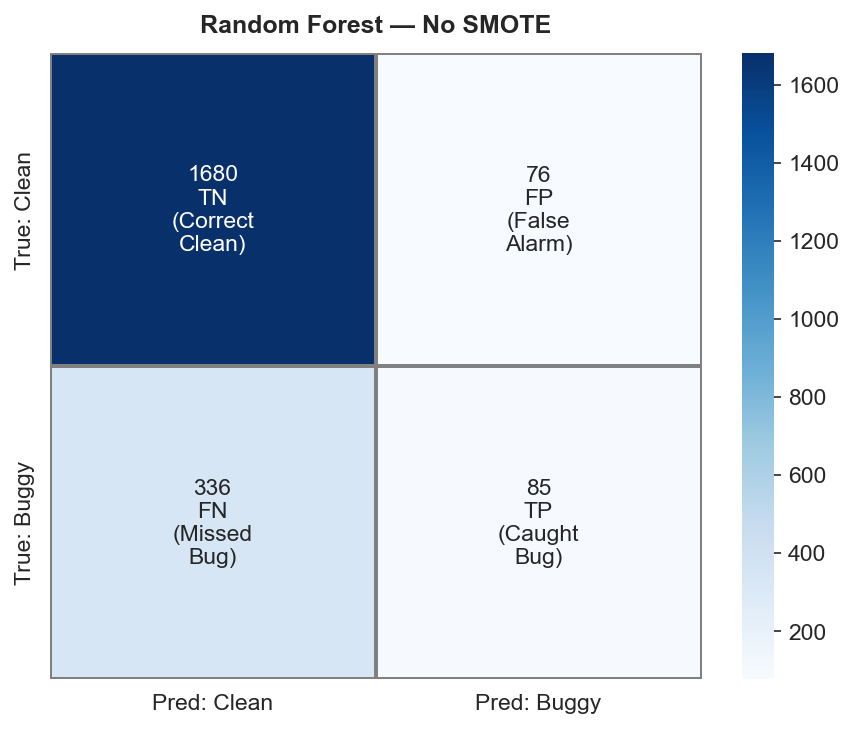
\includegraphics[width=\linewidth]{06_cm_rf_raw.png}
  \caption{Random Forest, no SMOTE}
\end{subfigure}
\hfill
\begin{subfigure}[b]{0.47\linewidth}
  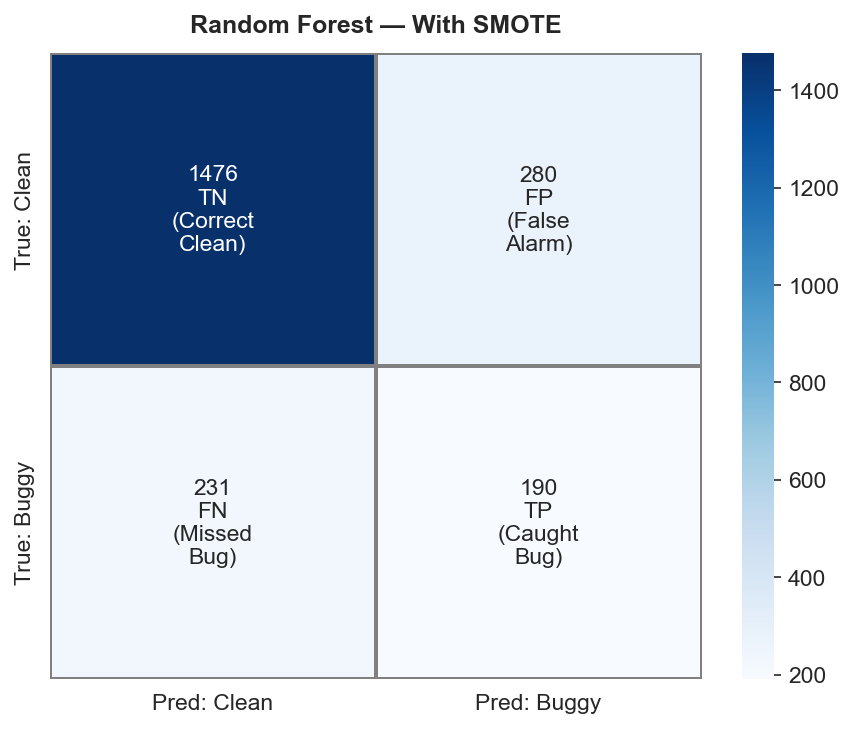
\includegraphics[width=\linewidth]{07_cm_rf_smote.png}
  \caption{Random Forest with SMOTE}
\end{subfigure}
\caption{Confusion matrices for the Random Forest configurations on the held-out test set}
\label{fig:cmrf}
\end{figure}

\begin{figure}[H]
\centering
\begin{subfigure}[b]{0.47\linewidth}
  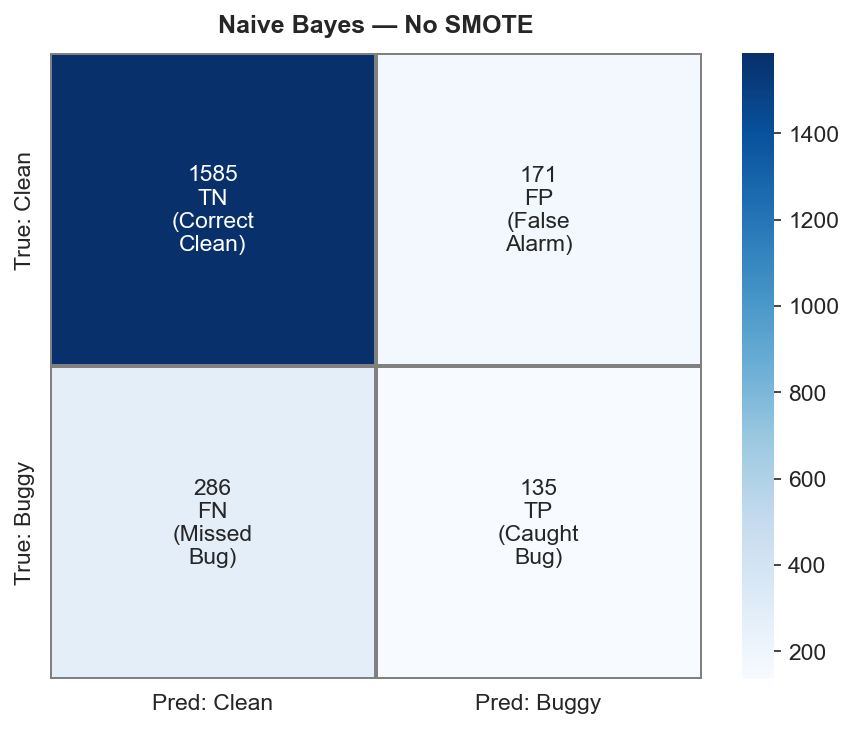
\includegraphics[width=\linewidth]{08_cm_nb_raw.png}
  \caption{Naive Bayes, no SMOTE}
\end{subfigure}
\hfill
\begin{subfigure}[b]{0.47\linewidth}
  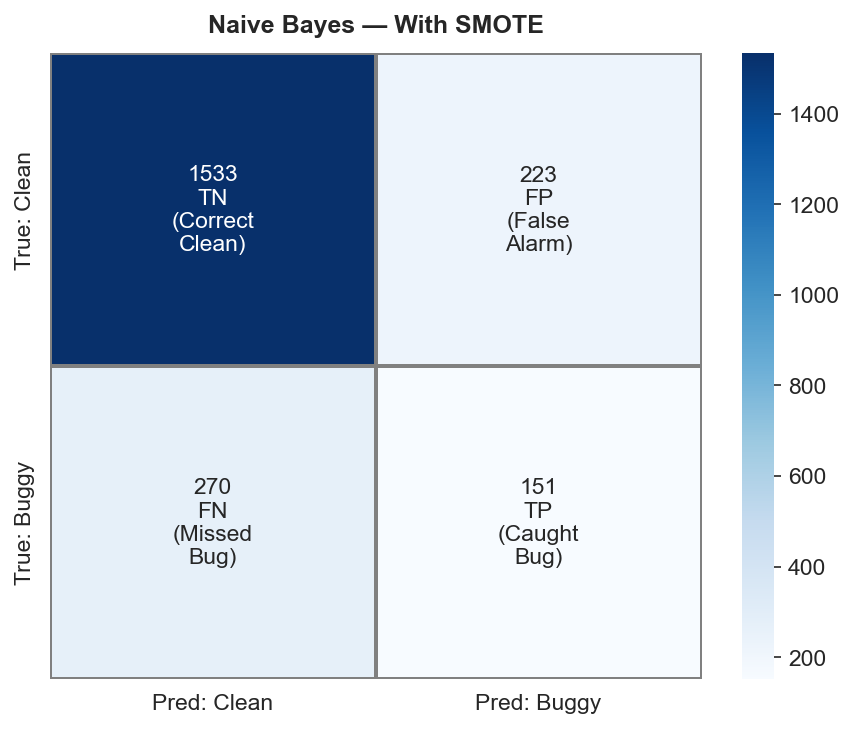
\includegraphics[width=\linewidth]{09_cm_nb_smote.png}
  \caption{Naive Bayes with SMOTE}
\end{subfigure}
\caption{Confusion matrices for the Gaussian Naive Bayes configurations on the held-out test set}
\label{fig:cmnb}
\end{figure}

\section{Random Forest Feature Importance}

\begin{figure}[H]
\centering
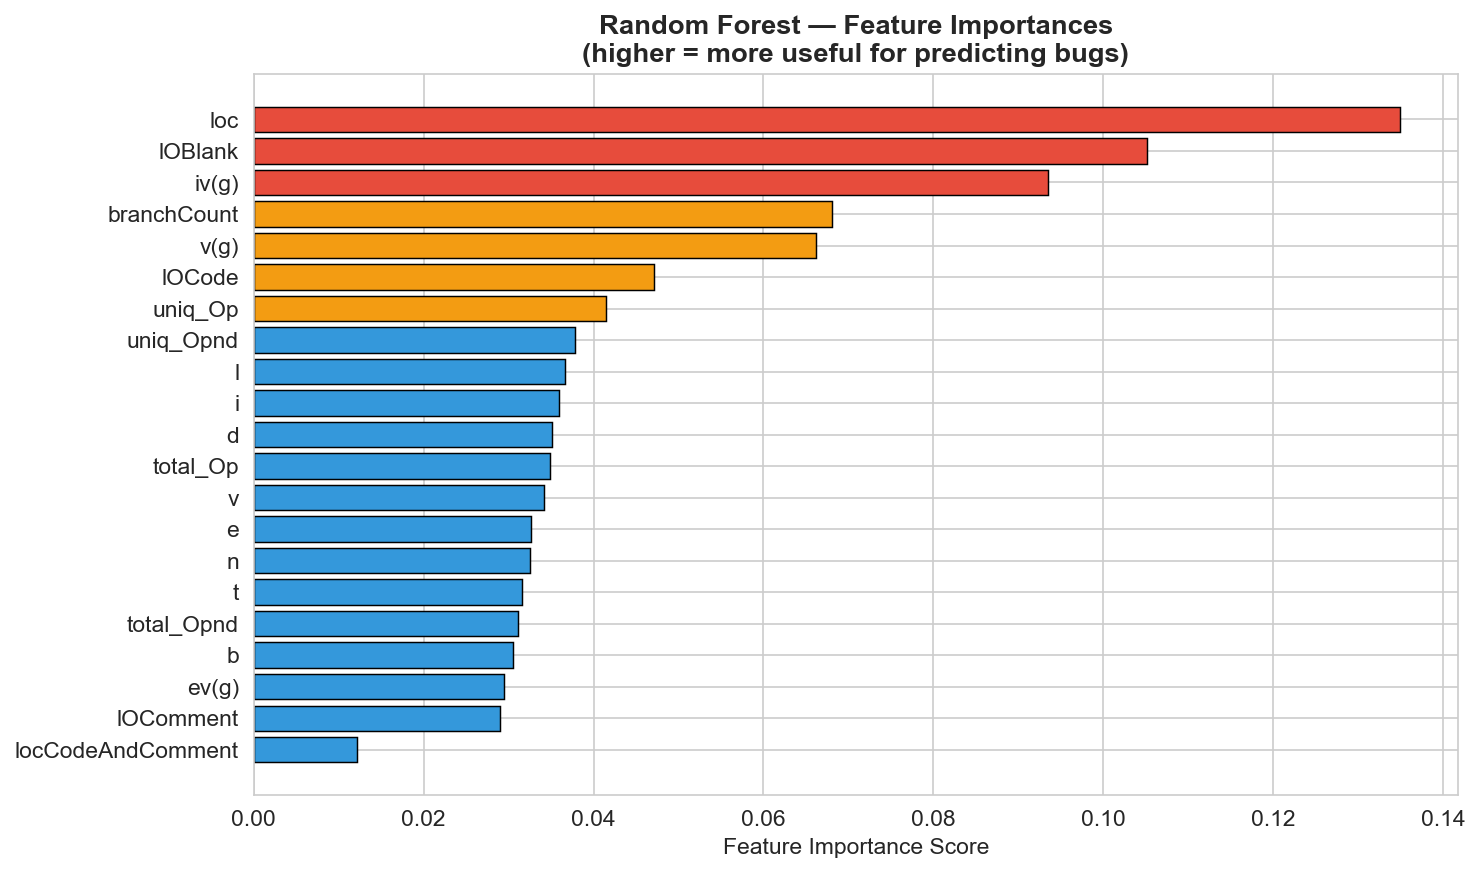
\includegraphics[width=0.88\linewidth]{10_feature_importance.png}
\caption{Gini importance of each complexity metric in the fitted Random Forest model}
\label{fig:featimp}
\end{figure}

\section{CNN-LSTM Training Dynamics}

\begin{figure}[H]
\centering
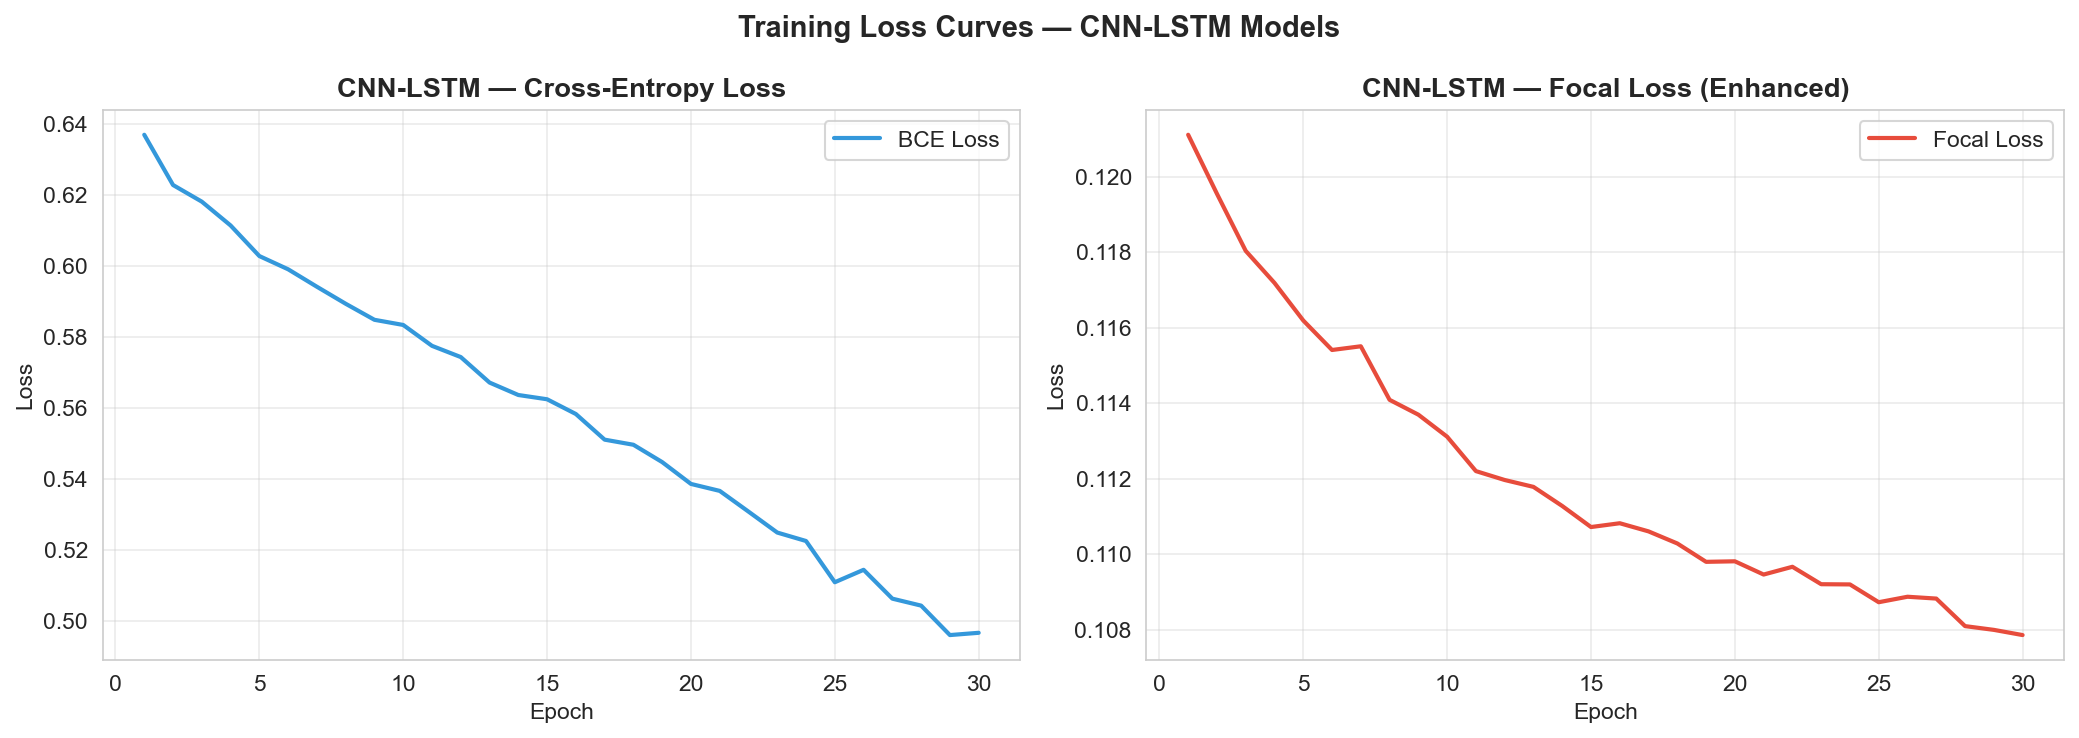
\includegraphics[width=0.88\linewidth]{12_cnnlstm_loss_curves.png}
\caption{Training and validation loss curves for the CNN-LSTM under binary cross-entropy and Focal Loss}
\label{fig:losscurves}
\end{figure}

\begin{figure}[H]
\centering
\begin{subfigure}[b]{0.47\linewidth}
  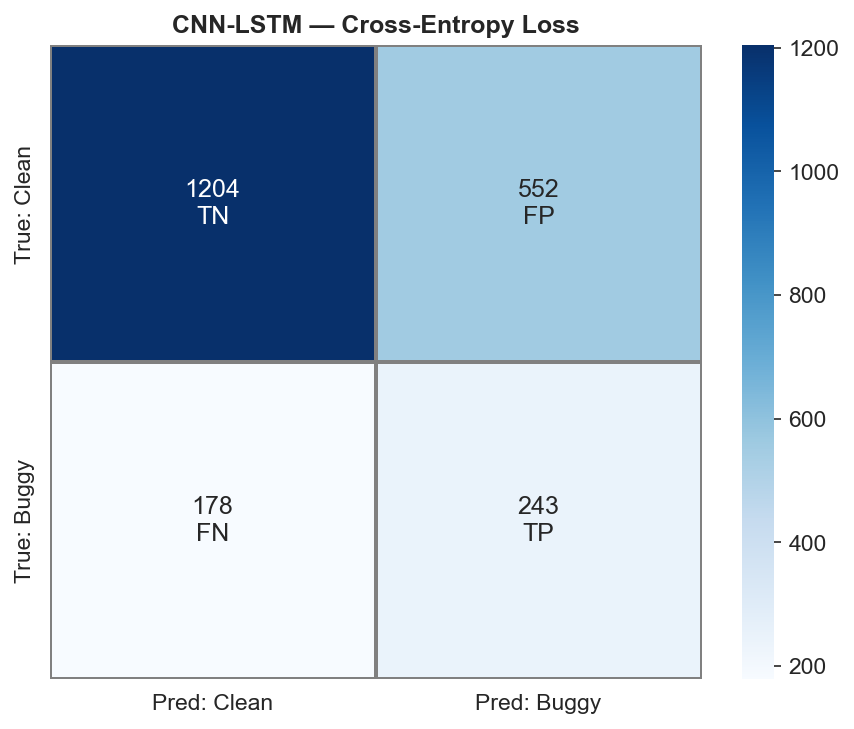
\includegraphics[width=\linewidth]{13_cm_cnnlstm_bce.png}
  \caption{CNN-LSTM, binary cross-entropy}
\end{subfigure}
\hfill
\begin{subfigure}[b]{0.47\linewidth}
  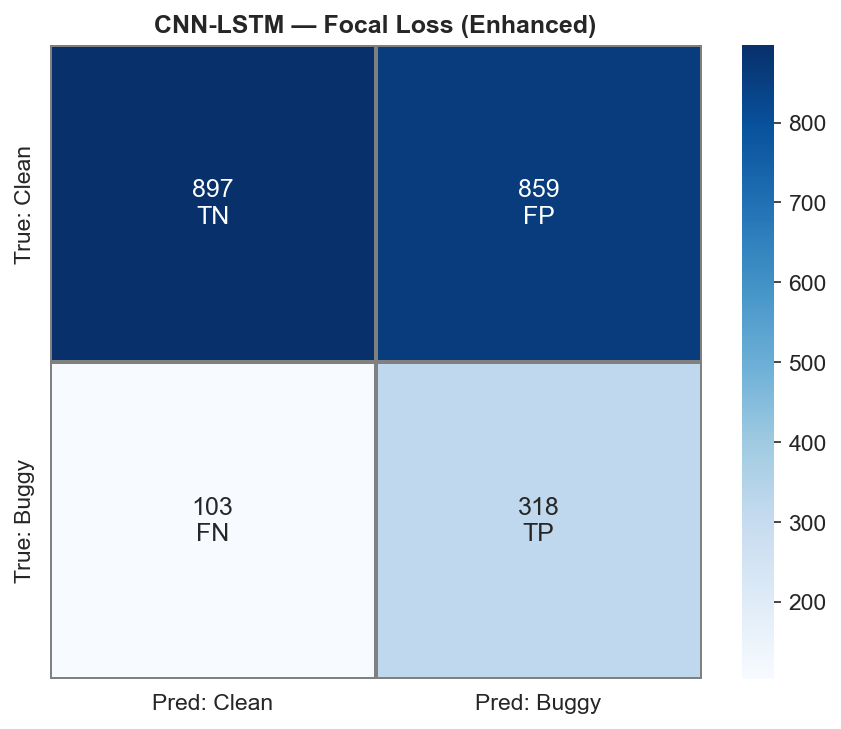
\includegraphics[width=\linewidth]{14_cm_cnnlstm_focal.png}
  \caption{CNN-LSTM, Focal Loss}
\end{subfigure}
\caption{Confusion matrices for the CNN-LSTM configurations on the held-out test set}
\label{fig:cmcnn}
\end{figure}

\section{DistilBERT Training and Evaluation}

\begin{figure}[H]
\centering
\begin{subfigure}[b]{0.47\linewidth}
  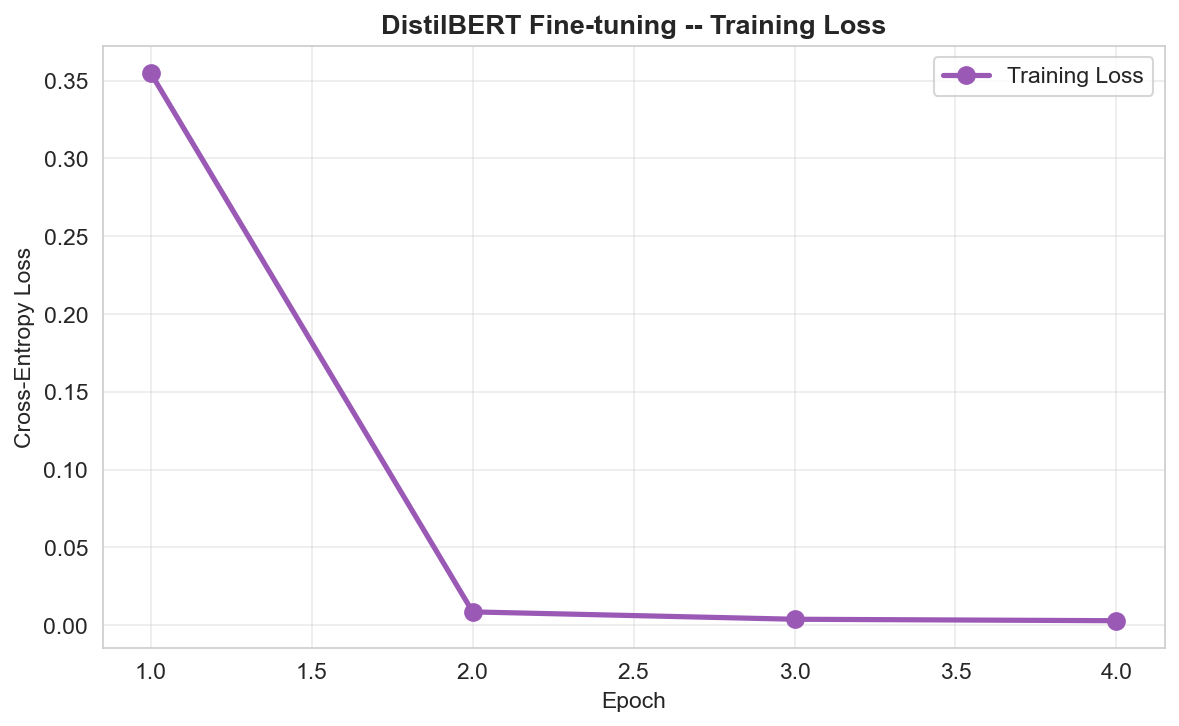
\includegraphics[width=\linewidth]{16_bert_loss_curve.png}
  \caption{Training loss across four epochs}
\end{subfigure}
\hfill
\begin{subfigure}[b]{0.47\linewidth}
  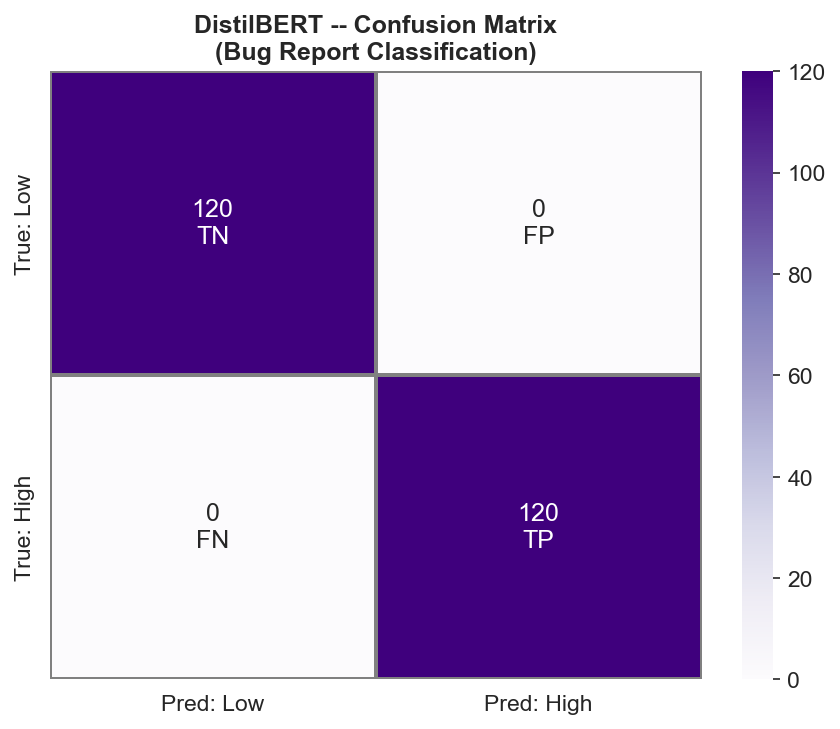
\includegraphics[width=\linewidth]{17_bert_confusion.png}
  \caption{Confusion matrix on the test set}
\end{subfigure}
\caption{DistilBERT training dynamics and test set evaluation on the bug report classification task}
\label{fig:bertfig}
\end{figure}

\section{Consolidated Model Comparison}

\begin{figure}[H]
\centering
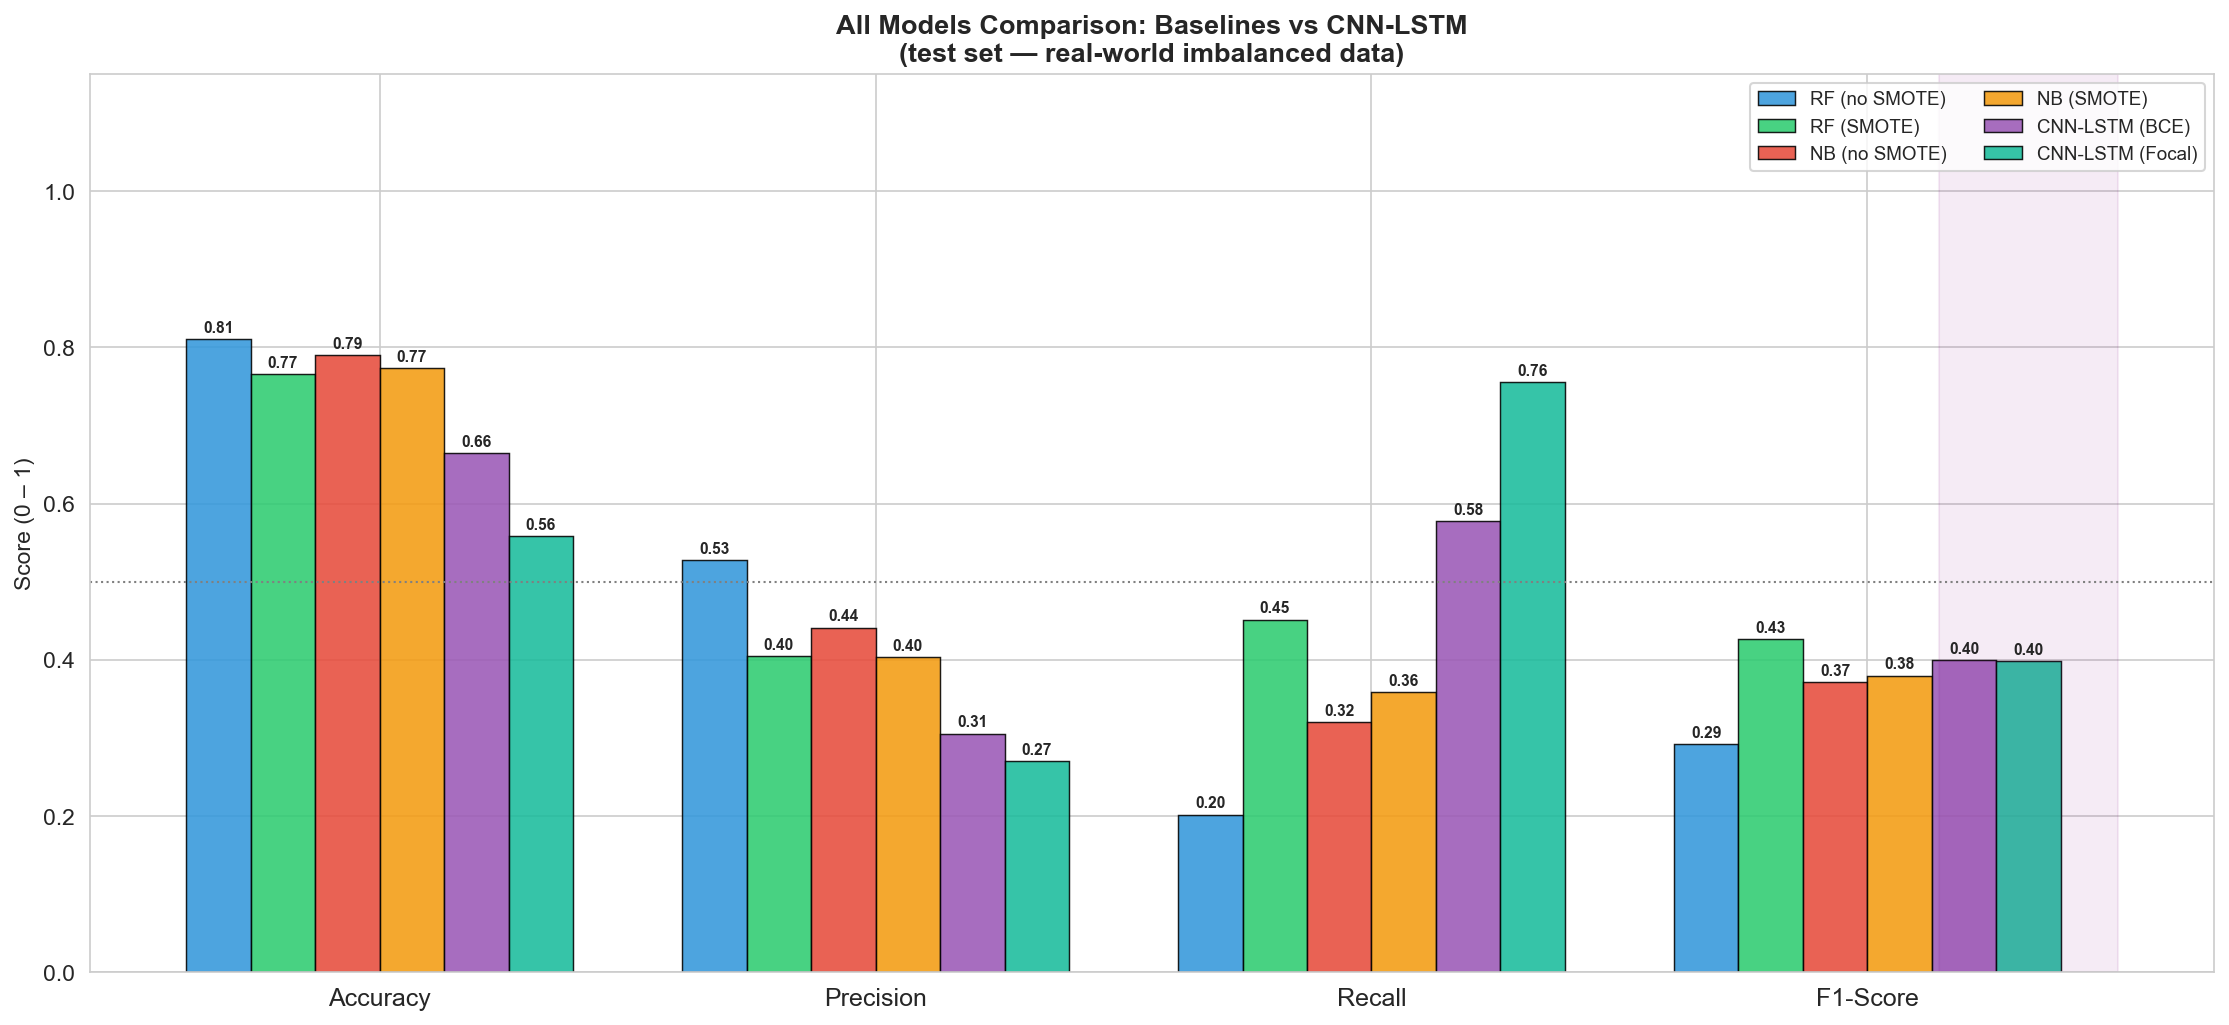
\includegraphics[width=0.95\linewidth]{15_all_models_comparison.png}
\caption{Consolidated comparison of all model configurations across the evaluation metrics}
\label{fig:allmodels}
\end{figure}

\clearpage

\chapter{Source Code Listings}
\label{app:b}

\section{Hybrid CNN-LSTM Model Definition}

\begin{lstlisting}[caption={Hybrid CNN-LSTM architecture implemented in PyTorch},label={lst:cnnlstm}]
class CNNLSTM(nn.Module):
    def __init__(self, input_size=21, hidden=64, num_filters=128):
        super().__init__()
        self.conv1 = nn.Conv1d(1, 64, kernel_size=3, padding=1)
        self.bn1   = nn.BatchNorm1d(64)
        self.conv2 = nn.Conv1d(64, num_filters, kernel_size=3, padding=1)
        self.bn2   = nn.BatchNorm1d(num_filters)
        self.lstm  = nn.LSTM(num_filters, hidden, batch_first=True)
        self.drop  = nn.Dropout(0.4)
        self.fc1   = nn.Linear(hidden, 32)
        self.fc2   = nn.Linear(32, 1)

    def forward(self, x):
        # x: (batch, 21, 1) -> (batch, 1, 21)
        x = x.transpose(1, 2)
        x = F.relu(self.bn1(self.conv1(x)))
        x = F.relu(self.bn2(self.conv2(x)))
        # (batch, filters, seq) -> (batch, seq, filters)
        x = x.transpose(1, 2)
        x, _ = self.lstm(x)
        x = self.drop(x[:, -1, :])
        x = F.relu(self.fc1(x))
        return torch.sigmoid(self.fc2(x)).squeeze()
\end{lstlisting}

\section{Class-Weighted Focal Loss}

\begin{lstlisting}[caption={Class-Weighted Focal Loss, the primary contribution of this study},label={lst:cwfl}]
class WeightedFocalLoss(nn.Module):
    """Focal Loss with an additional class-level weight set to the
    observed imbalance ratio of the training data."""

    def __init__(self, alpha=0.75, gamma=2.0, pos_weight=4.2):
        super().__init__()
        self.alpha      = alpha
        self.gamma      = gamma
        self.pos_weight = pos_weight

    def forward(self, inputs, targets):
        bce = F.binary_cross_entropy(inputs, targets, reduction='none')
        pt  = torch.exp(-bce)
        # Class-level weight: pos_weight for defective, 1.0 for clean
        weight = targets * self.pos_weight + (1 - targets) * 1.0
        # Example-level focusing
        focal  = self.alpha * (1 - pt) ** self.gamma * bce
        return (weight * focal).mean()
\end{lstlisting}

\section{Preprocessing Pipeline}

\begin{lstlisting}[caption={Five-stage preprocessing pipeline},label={lst:prep}]
# Stage 1: median imputation, fitted on training data only
imputer = SimpleImputer(strategy='median')

# Stage 2: winsorisation at the 99th percentile
def winsorize(df, p=99):
    for col in df.columns:
        cap = np.percentile(df[col], p)
        df[col] = np.clip(df[col], None, cap)
    return df

# Stage 3: stratified 80/20 partition
X_train, X_test, y_train, y_test = train_test_split(
    X, y, test_size=0.2, stratify=y, random_state=42)

# Stage 4: min-max normalisation, fitted on training data only
scaler   = MinMaxScaler().fit(X_train)
X_train  = scaler.transform(X_train)
X_test   = scaler.transform(X_test)

# Stage 5: BorderlineSMOTE, applied to training data only
smote = BorderlineSMOTE(random_state=42)
X_train_bal, y_train_bal = smote.fit_resample(X_train, y_train)
\end{lstlisting}

\clearpage

\chapter{Software and Hardware Specifications}
\label{app:c}

\begin{table}[H]
\centering
\caption{Complete software and hardware environment}
\label{tab:fullenv}
\tabfont
\begin{tabular}{L{55mm}L{75mm}}
\toprule
\textbf{Component} & \textbf{Version or specification} \\
\midrule
Operating system         & Windows 11 Home, build 26200 \\
Python                   & 3.13.2 \\
PyTorch                  & 2.12.0+cpu \\
scikit-learn             & 1.8.0 \\
imbalanced-learn         & 0.13.0 \\
HuggingFace Transformers & 5.9.0 \\
NumPy                    & 2.x \\
Pandas                   & 2.x \\
Matplotlib               & 3.x \\
Seaborn                  & 0.13.x \\
OpenML                   & 0.14.x \\
Hardware                 & CPU only, Intel-based workstation \\
Accelerator              & None \\
Random seed              & 42, fixed across all experiments \\
\bottomrule
\end{tabular}
\end{table}

\begin{table}[H]
\centering
\caption{Approximate training times on CPU hardware}
\label{tab:times}
\tabfont
\begin{tabular}{L{60mm}C{35mm}}
\toprule
\textbf{Experiment} & \textbf{Duration} \\
\midrule
Random Forest and Naive Bayes, all configurations & 30 minutes \\
CNN-LSTM, three loss configurations               & 60 minutes \\
DistilBERT fine-tuning, four epochs               & 24 minutes \\
Ten-fold cross-validation, baselines              & 18 minutes \\
\midrule
Total                                             & approx. 2 hours \\
\bottomrule
\end{tabular}
\end{table}

\clearpage

\chapter{Dataset Feature Dictionary}
\label{app:d}

\begin{table}[H]
\centering
\caption{Complete feature dictionary for the JM1 dataset}
\label{tab:dict}
\tabfont
\begin{tabular}{L{34mm}L{96mm}}
\toprule
\textbf{Feature} & \textbf{Description} \\
\midrule
\texttt{loc}              & McCabe count of lines of code \\
\texttt{v(g)}             & McCabe cyclomatic complexity \\
\texttt{ev(g)}            & McCabe essential complexity \\
\texttt{iv(g)}            & McCabe design complexity \\
\texttt{n}                & Halstead total operators plus operands \\
\texttt{v}                & Halstead program volume \\
\texttt{l}                & Halstead program length \\
\texttt{d}                & Halstead program difficulty \\
\texttt{i}                & Halstead intelligence content \\
\texttt{e}                & Halstead programming effort \\
\texttt{b}                & Halstead estimated delivered bugs \\
\texttt{t}                & Halstead estimated programming time \\
\texttt{lOCode}           & Halstead count of executable lines \\
\texttt{lOComment}        & Halstead count of comment lines \\
\texttt{lOBlank}          & Halstead count of blank lines \\
\texttt{lOCodeAndComment} & Count of lines containing both code and comment \\
\texttt{uniq\_Op}         & Number of unique operators \\
\texttt{uniq\_Opnd}       & Number of unique operands \\
\texttt{total\_Op}        & Total count of operators \\
\texttt{total\_Opnd}      & Total count of operands \\
\texttt{branchCount}      & Number of branches in the control flow graph \\
\midrule
\texttt{defects}          & Target variable: 1 if the module contains one or more reported defects, 0 otherwise \\
\bottomrule
\end{tabular}
\end{table}

\end{document}
